%\documentclass[final,5p,times,twocolumn,authoryear]{elsarticle}

% ----------- Removing the first page that causes trouble -----------
\usepackage{atbegshi}% http://ctan.org/pkg/atbegshi
\AtBeginDocument{\AtBeginShipoutNext{\AtBeginShipoutDiscard}}

% ----------- Define document class ---------------------------------
\documentclass[english, a4paper, 12pt, twoside]{article} 


\usepackage[utf8]{inputenc}
\usepackage[english]{babel}


% ----------- DEFINING COLOUR LINKS ---------------------
\usepackage{xcolor} % For colors
\usepackage{hyperref} % For hyperlinks
\hypersetup{
    colorlinks=true, % Set to true to enable colored links
    linkcolor={0 0.68 0.94}, % Internal links color (light blue)
    citecolor={0 0.68 0.94}, % Reference links color (light blue)
    urlcolor={0 0.68 0.94} % External URL links color (light blue)
}
\definecolor{lightlightgreen}{rgb}{0.9, 1, 0.9} % Very light green
\definecolor{lightlightred}{rgb}{1, 0.9, 0.9} % Very light red


% -------------- FORMATTING PAGE -------------------------
\linespread{1.5} % line spread for the document
\usepackage[margin=1in]{geometry} % defining the page margin

% --------------- FORMATTING THE APPENDIX ------------------
\usepackage[titletoc,title]{appendix}
\newcommand{\appref}[1]{Appendix~\ref{#1}}

% -------------- PACKAGES FOR FORMATTING TABLES AND IMAGES -----------
\usepackage{rotating}
\usepackage{algpseudocode}
\newcommand{\algorithmautorefname}{Algorithm}
\usepackage{longtable} % formatting for large tables
\usepackage{amssymb}
\usepackage{tabularx}  % important for table formatting
\usepackage{graphicx}  % important for figure formatting
\setkeys{Gin}{width=\linewidth,keepaspectratio} % for table and image format
\newcommand{\kms}{km\,s$^{-1}$} % for table and image format
\newcommand{\msun}{$M_\odot} % for table and image format
\titleformat{\section}
  {\bfseries\LARGE}{\thesection}{1em}{}  
\usepackage{booktabs} % for better table formatting
\usepackage{subcaption} % for subfigures

%\usepackage{array}

%------ APCKAGES FROM NHH TEMPLATEW --------------------

\addcontentsline{toc}{section}{00 bib.bib}

\usepackage{textcomp}
\usepackage[T1]{fontenc, url}
\usepackage[utf8]{inputenc}
\usepackage{titlesec}
\setcounter{secnumdepth}{4}
\usepackage{multirow}
%\usepackage{minted} % Code highlighting
\usepackage{adjustbox}
\usepackage{graphicx}
\usepackage{amsmath, amssymb, amsthm} % Mathematical packages
\usepackage{parskip} % Removing indenting in new paragraphs
\urlstyle{sf}
\usepackage{color}
\usepackage{subcaption} 
\usepackage{appendix}
\usepackage{chngcntr} % needed for correct table numbering
\counterwithin{table}{section} % numbering of tables 
\counterwithin{figure}{section} % numbering of figures
\numberwithin{equation}{section} % numbering of equations
\hyphenpenalty=100000 % preventing splitting of words
\sloppy 
\raggedbottom 
\usepackage{xparse,nameref}

\usepackage{fancyhdr}
\usepackage{subfiles}
\usepackage{array}
\usepackage[rightcaption]{sidecap}
\usepackage{wrapfig}
\usepackage{float}
\usepackage[labelfont=bf]{caption} % bold text for captions
\usepackage[para]{threeparttable} % fancy tables, check these before you use them
\usepackage{url}
\usepackage[table,xcdraw]{xcolor}
\usepackage{makecell}
\usepackage{hhline}

% ------------- FORMATTING HEADER --------------------------
%\usepackage{fancyhdr}
%\pagestyle{fancy}
%\fancyhf{}
\pagestyle{fancy}
\fancyhead[RE,LO]{\thepage} % page number on right for odd pages and left for even pages in the header
\fancyhead[RO,LE]{\nouppercase{\leftmark}} % chapter name and number on the right for even pages and left for odd pages in the header
%\renewcommand{\headrulewidth}{0pt} % sets thickness of header line
\fancyfoot{} % removes page number on bottom of page

% ----------- DEFINING HYPER REF COLOURS --------------------
\usepackage{hyperref}
\hypersetup{
    colorlinks=true, % Enables colored links
    linkcolor=blue, % Internal links color
    citecolor=blue, % Reference links color (for citations)
    urlcolor=blue % External URL links color
}


% -------------- CODE SNIPPETS -------------------------------
\usepackage{listings} % for code listings
\lstset{
  basicstyle=\ttfamily,
  breaklines=true,
  postbreak=\mbox{\textcolor{red}{$\hookrightarrow$}\space},
}

\usepackage{algorithm} % for algorithms
\usepackage{algorithmicx} % for algorithms
\usepackage{microtype} % for micro-typographical adjustments
\usepackage{footnote} % for footnotes
\usepackage{marginnote} % for side notes
\usepackage{amsmath}
\usepackage{amsfonts}
\usepackage{bm}
\usepackage{makecell} % To make cells more spacious
\usepackage{multirow} % For multi-row cells
\usepackage{multicol}
\usepackage{amssymb}
\usepackage{tabularx}
\usepackage{titlesec}

% ----------- DEFINE MATH FONT -----------------
\usepackage{unicode-math}
\setmathfont{Latin Modern Math} % using a math font


% \usepackage{stfloats}

% ----------- FORMATTING CATIONS -----------------
\usepackage{caption}
\setlength{\abovecaptionskip}{0pt}
\setlength{\belowcaptionskip}{0pt}
\usepackage[labelfont=bf]{caption} % Keeps captions bold in the text
\usepackage[font=footnotesize]{caption} 

% formatting subcaption using the subcaption package
\usepackage{subcaption}
\usepackage[font=footnotesize]{subcaption} 
%\usepackage[font=singlespacing]{subcaption}

\usepackage{setspace}
\newcommand{\mylinespacedsubcaption}[1]{
    \begin{spacing}{0.8} % Adjust the 0.8 to your preferred line spacing
    \subcaption{#1}
    \end{spacing}
}
\usepackage[labelfont=bf]{caption}

% -----------------ADDING BLANK PAGE AFTER COVER --------------------
\usepackage{afterpage}

\newcommand\blankpage{%
    \null
    \thispagestyle{empty}%
    \addtocounter{page}{-1}%
    \newpage}

%--------------- FORMATTING TABLE OF CONTENT ----------------------
%\usepackage{tocloft}
% Change the link color temporarily for TOC, LOF, and LOT
\renewcommand{\cftsecfont}{\hypersetup{linkcolor=blue}\normalfont}
\renewcommand{\cftsubsecfont}{\hypersetup{linkcolor=blue}\normalfont}
\renewcommand{\cftsecpagefont}{\hypersetup{linkcolor=blue}\normalfont} % for page numbers
\renewcommand{\cftsubsecpagefont}{\hypersetup{linkcolor=blue}\normalfont} % for page numbers
\setcounter{tocdepth}{2} % setting the level of TOC to display
%\usepackage{tocloft}

% ---------------- USE THIS TO ADJUST SIZE AND SPACE IN TOC ---------
\usepackage[titles]{tocloft}
\setlength{\cftbeforesecskip}{-1.1ex}
\setlength{\cftbeforesubsecskip}{-1.1ex}

\renewcommand{\cftsecfont}{\small\bf}
\renewcommand{\cftsubsecfont}{\small}
\renewcommand{\cftsubsubsecfont}{\small}

% ---- FORMATIN LIST OF FIGURES
\renewcommand{\cftfigfont}{\small}
\setlength{\cftbeforefigskip}{-1ex}

% ---- FORMATIN LIST OF TABLES
\setlength{\cftbeforetabskip}{-1ex}
\renewcommand{\cfttabfont}{\small}

\captionsetup[figure]{font=bf}
\captionsetup[table]{font=bf}


\usepackage{rotating}

\usepackage{listings}


% Change font size for subsections in TOC
%\renewcommand{\cftsubsecfont}{\small}

% Change font size for subsubsections in TOC
%\renewcommand{\cftsubsubsecfont}{\footnotesize}


% Reduce line spacing for sections in TOC
%\setlength{\cftbeforesecskip}{1pt}

% Reduce line spacing for subsections in TOC
%\setlength{\cftbeforesubsecskip}{0pt}

% Reduce line spacing for subsubsections in TOC
%\setlength{\cftbeforesubsubsecskip}{0pt}

% Change font style for List of Figures entries to normal (not bold)
%\renewcommand{\cftfigfont}{\normalfont}

% Change font style for List of Tables entries to normal (not bold)
%\renewcommand{\cfttabfont}{\normalfont}


% Change font style for List of Figures entries to normal (not bold) and reduce the font size
%\renewcommand{\cftfigfont}{\normalfont\small}

% Ensure that the page numbers in LOF are also not bold
%\renewcommand{\cftfigpagefont}{\normalfont\small}



%\usepackage{colortbl}













% bibliography using APA
\usepackage[style=apa, backend=biber, natbib=true]{biblatex}

\addbibresource{00 bib.bib} % Make sure this matches the name of your BibTeX file
\setlength{\parskip}{1em} % Adjusts the space between paragraphs
\setlength{\parindent}{0pt} % Removes indentation at the

%\usepackage[font=singlespacing]{subcaption}




% Begin document


% adding correct page number formatting
\pagenumbering{roman}

\begin{document}


% Custom Cover Page
\begin{titlepage}
    % Logo in the top left corner

    % FIGUR FIGUR FIGUR %
    \begin{minipage}{0.25\textwidth}
        
\includegraphics[width=0.5\linewidth]{images/nhh_logo.png}
    \end{minipage}
    \hfill 
    % Larger text in the top right corner
    \begin{minipage}{0.6\textwidth}
        \flushright \normalsize Norwegian School of Economics\\
        Bergen, Autumn 2023
    \end{minipage}

    \vspace{2cm} % Adjust this value to position the title higher or lower

    \begin{center}
        % Title in bold and large font
        \textbf{\LARGE 
        Exploiting the Index Effect on OSEBX \\
        using Machine Learning}
        \vspace{1em}
        
        % Subtitle in cursive and smaller font
        {\Large \textit{Trading on predictions made by GLM and XGBoost with a conditional posterior probability threshold}}
        
        \vspace{2cm}
        
        % Authors in bold and large font
        \textbf{\Large Arne Jordåen \& Egil Furnes}
        
        \vspace{0.5em}
        
        % Supervisor detail with increased size
        \textbf{{\Large Supervisor: Sondre Nedreås Hølleland}}

        \vspace{1.5cm}
        
        % Additional details and lines in normal font
        Master thesis, Economics and Business Administration\\
        Major: Business Analytics\\
        NORWEGIAN SCHOOL OF ECONOMICS
    \end{center}

    \vfill

    \begin{center}
    \parbox{0.9\textwidth}{ \small
        This thesis was written as a part of the Master of Science in Economics and Business Administration at NHH. Please note that neither the institution nor the examiners are responsible – through the approval of this thesis – for the theories and methods used, or results and conclusions drawn in this work.
    }
\end{center}
\end{titlepage}


\clearpage
\thispagestyle{empty}
\hfill

\clearpage% 
\begin{frontmatter}

\title{Predicting and trading on additions and deletions to Oslo Stock Exchange Benchmark Index using XGBoost with a custom objective function}

\author[first]{Arne Jordåen}
\author[first]{Egil Furnes}

\affiliation[first]{
            organization={Norwegian School of Economics},
            addressline={Helleveien 30}, 
            city={Bergen},
            postcode={5045}, 
            state={Vestland},
            country={Norway}}
%

\begin{abstract}
    \section*{Abstract}

In March and September of each year, Euronext decide which companies should be included on the Oslo Stock Exchange Benchmark Index (OSEBX). OSEBX consists of 50-80 companies, all selected from the approximately 200 companies on the Oslo Stock Exchange All Shares Index (OSEAX). We find that new additions and deletions to OSEBX experience significant price effects leading up to the actual date these changes take place, the effective date (ED). These price effects are named the \textit{index effect}.

We use the machine learning (ML) models \textit{eXtreme Gradient Boosting} (\textit{XGBoost}) and \textit{Generalised Linear Model} (\textit{GLM}) to predict index composition to OSEBX in the months leading up to ED. We find that both XGBoost and GLM can predict index composition with accuracy higher than 94\%, 30, 60, and 100 days in advance of ED.

Next, we simulate portfolios from 2010 to 2022, buying predicted additions and selling predicted deletions. We find that GLM models predict few, but high-yielding companies. XGBoost models predict more additions and deletions and create more diverse portfolios. The best GLM and XGBoost portfolios outperformed OSEBX by respectively 0.95\% and 0.32\% per month (11.4\% and 3.84\% per year) in the period from 2010 to 2022. Even after adjusting for risk in a Fama-French 3 Factor Model (FF3), the same portfolios showed significant alphas at a 95\% confidence level.

Lastly, we investigate if the same active trading strategy can yield excess returns in an enhanced index portfolio. In practice, we did this by combining the already simulated portfolios with OSEBX, where we optimised the active share of the portfolio to give the combined portfolio a tracking error of 2\%. For the enhanced index portfolios, the best GLM and XGBoost portfolios outperformed OSEBX by respectively 0.05\% and 0.06\% per month (0.6\% and 0.72\% per year). However, after adjusting for risk factors in FF3 only one of the XGBoost portfolios showed a significant alpha ($p$-value < 0.1).

In short, we find that ML models can predict upcoming changes to OSEBX with high accuracy and that exploiting the index effect using ML can yield excess returns. 



\end{abstract}

\begin{keyword}
Index Effect \sep Enhanced Index Investing \sep Machine Learning \sep eXtreme Gradient Boosting (XGBoost) 
\end{keyword}

\end{frontmatter}
\newpage

\section*{Acknowledgements}


This thesis was written in the autumn of 2023, as part of our master of science degree in Economics and Business Administration with a major in Business Analytics from NHH. 

We would like to thank our supervisor, Assistant Professor Sondre Nedreås Hølleland, for providing valuable feedback and support throughout the semester. Furthermore, we would like to thank Assistant Professor Andreas Ørpetveit for his feedback and support for the financial aspects of our thesis. We greatly appreciate the encouraging discussions with them both. 

Arne would like to thank Nicholas de Flon for rewarding discussions regarding the methodology and inspiration of this thesis. 

Egil would like to thank the portfolio managers and trading desk, and the index investment team led by Eivind Aukrust at DNB Asset Management for introducing the relevant topics of this thesis and providing practical insights. 

We are thankful to family and friends during this semester, which has provided great encouragement along the way. Also, we extend a special thanks to our good friends from Stafettkomitéen NHHS, for helping us stay on track and keep moving forward. 

\vspace{1in} % Adjust vertical space as needed

\begin{center}
    Norwegian School of Economics 
\end{center}
\begin{center}
    Bergen, December 2023 
\end{center}

\vspace{1in} % Adjust vertical space as needed
\noindent
\makebox[2.5in]{\hrulefill} \hfill \makebox[2.5in]{\hrulefill} \\
\makebox[2.5in][c]{Arne Jordåen} \hfill \makebox[2.5in][c]{Egil Furnes}

\newpage
\section*{Abstract}

In March and September of each year, Euronext decide which companies should be included on the Oslo Stock Exchange Benchmark Index (OSEBX). OSEBX consists of 50-80 companies, all selected from the approximately 200 companies on the Oslo Stock Exchange All Shares Index (OSEAX). We find that new additions and deletions to OSEBX experience significant price effects leading up to the actual date these changes take place, the effective date (ED). These price effects are named the \textit{index effect}.

We use the machine learning (ML) models \textit{eXtreme Gradient Boosting} (\textit{XGBoost}) and \textit{Generalised Linear Model} (\textit{GLM}) to predict index composition to OSEBX in the months leading up to ED. We find that both XGBoost and GLM can predict index composition with accuracy higher than 94\%, 30, 60, and 100 days in advance of ED.

Next, we simulate portfolios from 2010 to 2022, buying predicted additions and selling predicted deletions. We find that GLM models predict few, but high-yielding companies. XGBoost models predict more additions and deletions and create more diverse portfolios. The best GLM and XGBoost portfolios outperformed OSEBX by respectively 0.95\% and 0.32\% per month (11.4\% and 3.84\% per year) in the period from 2010 to 2022. Even after adjusting for risk in a Fama-French 3 Factor Model (FF3), the same portfolios showed significant alphas at a 95\% confidence level.

Lastly, we investigate if the same active trading strategy can yield excess returns in an enhanced index portfolio. In practice, we did this by combining the already simulated portfolios with OSEBX, where we optimised the active share of the portfolio to give the combined portfolio a tracking error of 2\%. For the enhanced index portfolios, the best GLM and XGBoost portfolios outperformed OSEBX by respectively 0.05\% and 0.06\% per month (0.6\% and 0.72\% per year). However, after adjusting for risk factors in FF3 only one of the XGBoost portfolios showed a significant alpha ($p$-value < 0.1).

In short, we find that ML models can predict upcoming changes to OSEBX with high accuracy and that exploiting the index effect using ML can yield excess returns. 



\newpage



\tableofcontents\thispagestyle{fancy}
\newpage
\listoffigures\thispagestyle{fancy}
\newpage

\listoftables\thispagestyle{fancy}
\newpage

% Main text
\pagenumbering{arabic}
\section{Introduction}
\label{introduction}


The last 20 years have seen a massive increase in flows from \textit{active investing} strategies trying to outperform a given benchmark index, towards \textit{passive index investing} strategies trying to replicate a benchmark index \parencite{jpmorgan-exchange-traded-funds-etfs}. In this era, new index investing methods have emerged \parencite{jorion-enhanced-index-funds-and-tracking-error-optimization}. \textit{Enhanced index investing} is one such method, seeking to replicate the benchmark risk while outperforming the benchmark return \parencite{investopedia-passive-and-active-funds}. In this pursuit, enhanced index funds have found positive excess returns from exploiting the price effects of stocks being added or deleted from their benchmark index \parencite{nbim-investing-in-equities}. These price effects were first observed by \textcite{shleifer-do-demand-curves-for-stocks-slope-down} on the benchmark index S\&P 500, and subsequently named the S\&P phenomenon, or the \textit{index effect}. Since the discovery of the index effect by \textcite{shleifer-do-demand-curves-for-stocks-slope-down}, it has been investigated further \parencite{lynch-new-evidence-s&p-500}, and observed on other benchmark indices \parencite{afego-effects-of-changes-in-stock-index-composition}. In \autoref{fig:index-effect-osebx} we illustrate the average price movement of additions and deletions from 2002 to 2023 on the Oslo Stock Exchange Benchmark Index (OSEBX). 
\vspace{-1.3em}
\begin{figure}[H]
    \centering
    \makebox[\linewidth][c]{\hspace{-0.6em}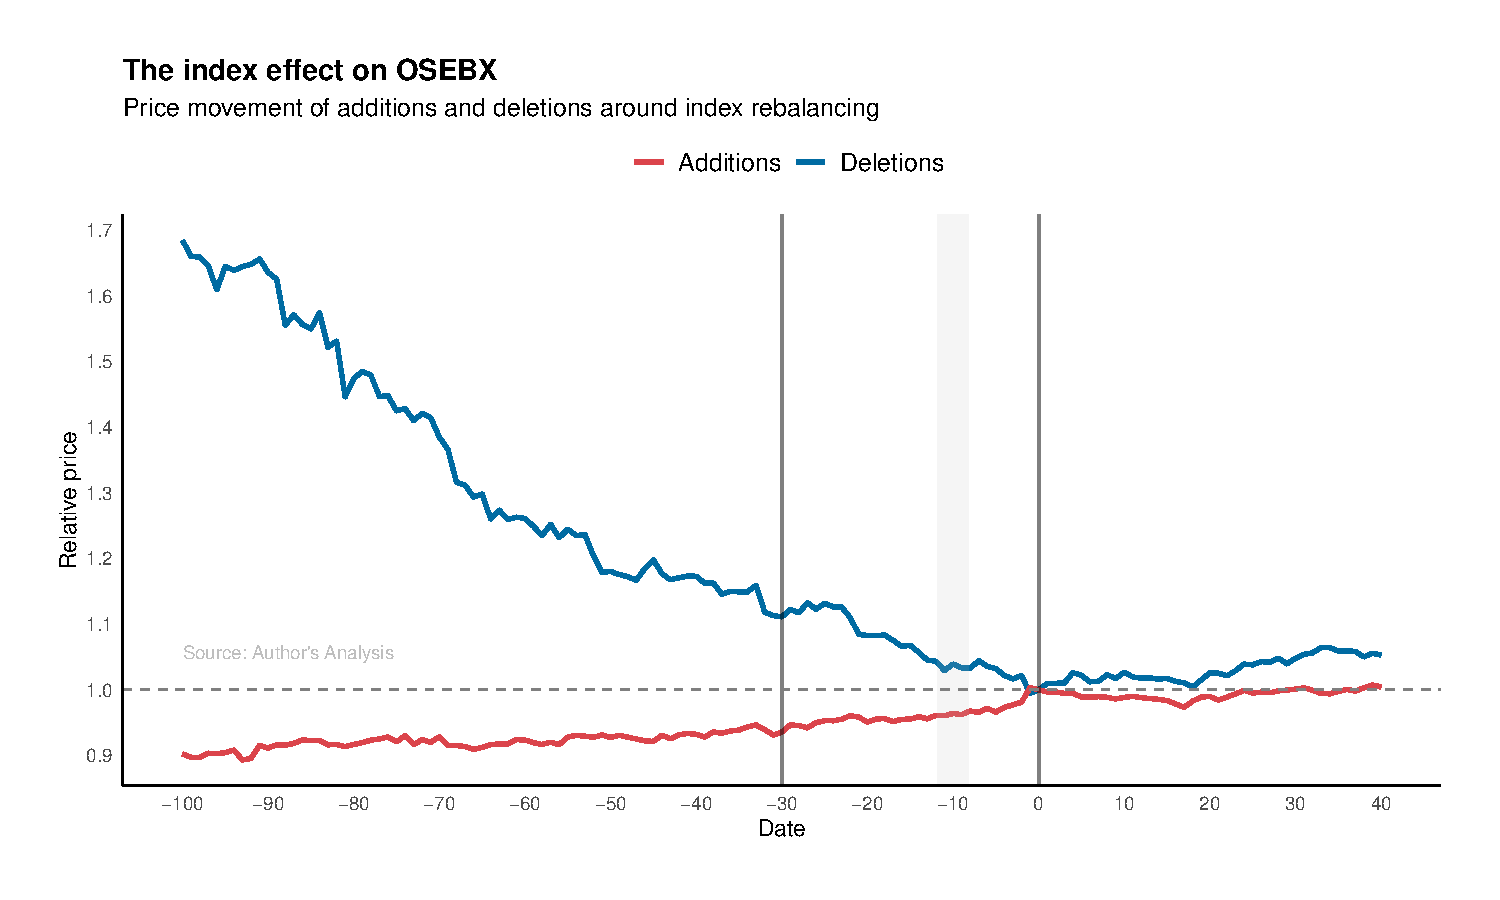
\includegraphics[width=1.0\textwidth]{images/index_plot_updated.pdf}}
    \caption{The Index Effect on OSEBX}
    \subcaption*{
     Illustration of aggregated relative price movements to the first effective day (day 0) with additions and deletions for OSEBX from 2002 to 2023. Day 0 represents the first day after the effective date (ED). The announcement date is typically 14 days ahead of the ED, and the data cutoff date (the day data is extracted for each company, which determines the index composition) is about 30 days in advance of the ED. The figure is generated using price data from Bloomberg.}
    \label{fig:index-effect-osebx}
\end{figure}

Similar to \textcite{shleifer-do-demand-curves-for-stocks-slope-down}, \autoref{fig:index-effect-osebx} shows that the stock price of additions typically increases in the period before being added to the benchmark index, with the equivalent opposite effect for deletions. There have also been some master's theses indicating the existence of such an effect on OSEBX, among those by \textcite{cbs-thesis-price-and-volume-effects-osebx} and \textcite{nhh-thesis-exploiting-the-index-effect-to-extract-alpha}. In short, \autoref{fig:index-effect-osebx} shows our illustration of the index effect on OSEBX since 2002. 

In March and September of each year, Euronext decides which companies should be on OSEBX. This event is guided by three dates, the cut-off date (CD), announcement date (AD), and effective date (ED) \parencite{OSEBX-rule-book}. The CD represents the day Euronext extracts data to use for the index rebalancing event. The index composition is announced on AD and implemented on ED. There are typically a few weeks between CD-AD and AD-ED. \autoref{fig:returns-for-additions-and-deletions-on-osebx} illustrate returns on OSEBX additions and deletions in the 50 days surrounding ED, indicating abnormal returns on ED.  

\vspace{-0.9em}
\begin{figure}[h]
    \centering
    
    \makebox[\linewidth][c]{\hspace{-0.6em}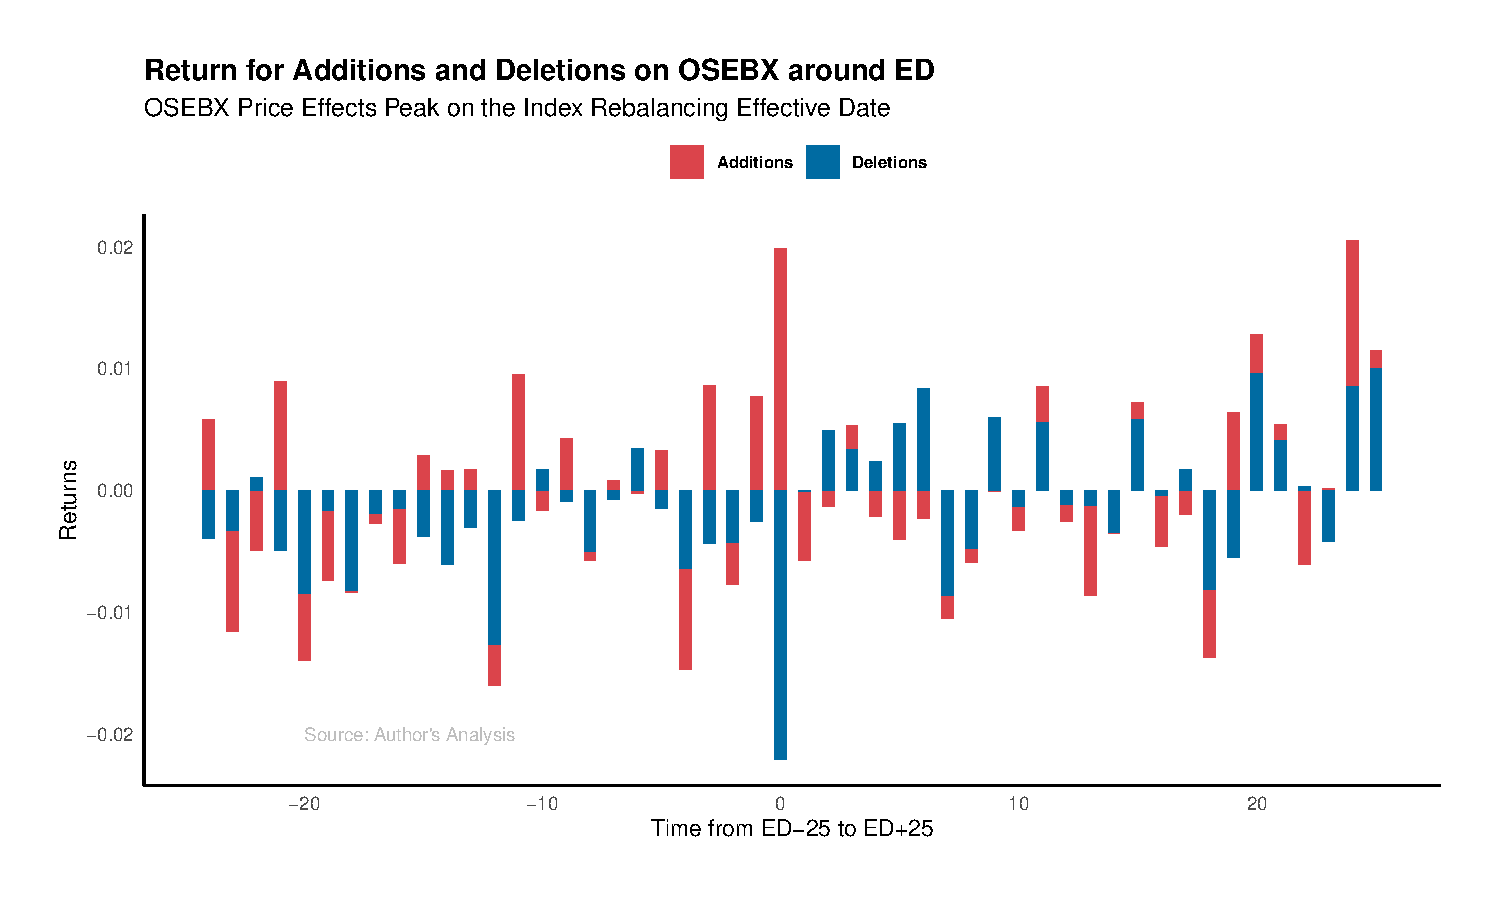
\includegraphics[width=1.06\textwidth]{images/retplot.pdf}}
    \caption{{Return for Additions and Deletions on OSEBX around ED}}
    \subcaption*{We illustrate the aggregated returns for additions and deletions to OSEBX from 2002 to 2023. The figure indicates abnormal returns for both additions and deletions on ED. The return on additions/deletions seems to rise/fall before ED, and somewhat readjust after ED.}
    \label{fig:returns-for-additions-and-deletions-on-osebx}
\end{figure}

In this thesis, we use machine learning (ML) to predict upcoming 
\textit{additions} and \textit{deletions} to OSEBX ahead of AD. Additions are companies not currently on OSEBX, which enter from one period to the next, and deletions are companies exiting OSEBX from one period to the next. By predicting before the AD, we can potentially obtain a competitive edge against competing investors who rely on the information announced on the AD. Then, we simulate a trading period from 2010 to 2022, which includes 22 distinct index rebalancing events. \autoref{fig-OSEBX-Number-of-Additions-and-Deletions} illustrate the changes we seek to capture. We use \textit{eXtreme Gradient Boosting} (\textit{XGBoost}) \parencite{xgboost-a-scaleable-tree-boosting-system} and a \textit{Generalised Linear Model} (\textit{GLM)} \parencite{glm-generalized-linear-models} to predict index composition in the next period. Next, we proceed with some definitions and brief reviews of the most common terms used in this thesis. 

\vspace{-0.9em}
\begin{figure}[h]
    \centering
    \makebox[\linewidth][c]{\hspace{-0.6em}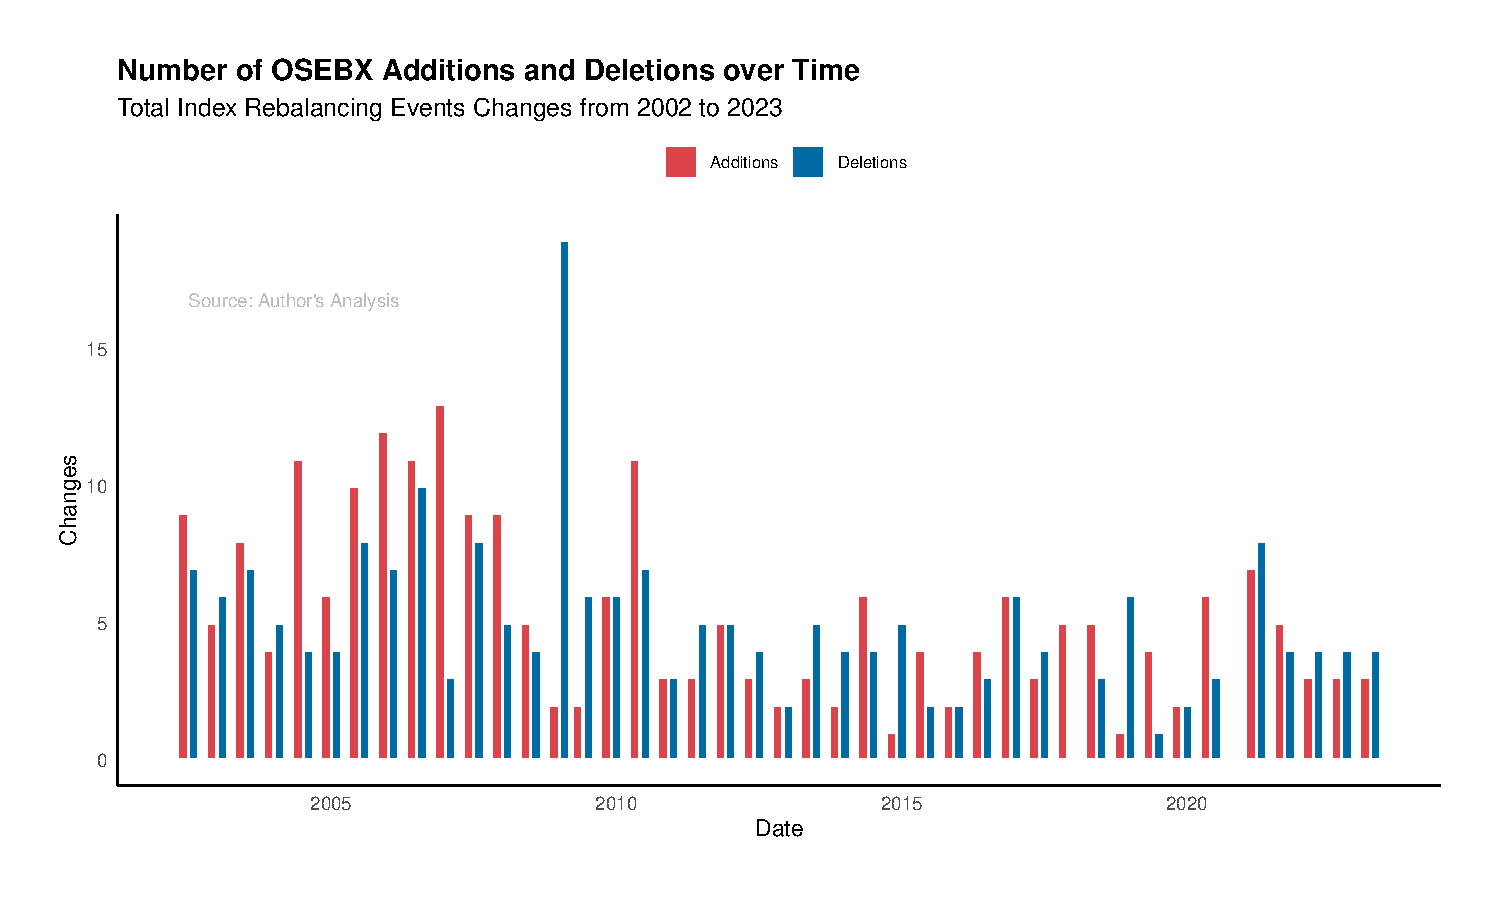
\includegraphics[width=1.06\textwidth]{images/plot_add_del.pdf}}
    \caption{{Number of OSEBX Additions and Deletions Over Time}}
    \subcaption*{Illustration of the number of additions and deletions to OSEBX in the period from 2002 to 2023. Typically, there are between 5-10 additions and deletions per index rebalancing event. We see quite a large number of deletions from OSEBX during the financial crisis.}
    \label{fig-OSEBX-Number-of-Additions-and-Deletions}
\end{figure}

The world saw its first index investing fund with John Bogle and the Vanguard 500 Index Fund in 1975 \parencite{vanguard-first-mutual-fund}. It was first of its kind in replicating a benchmark index and was mocked as Bogle's Folly. Since then, the fund has seen redemption by generating exceptional returns \parencite{vanguard-first-mutual-fund}. A benchmark index is a grouping of carefully selected assets, to represent the movement of the entire stock market \parencite{goel-index-tracking-and-enhanced-indexing-using-mixed-conditional-value-at-risk}. 

\textcite{afego-effects-of-changes-in-stock-index-composition} find differences in benchmark index transparency. The low transparency S\&P 500 has an undisclosed replacement pool and performs need-based rebalancing \parencite{afego-effects-of-changes-in-stock-index-composition}. OSEBX, on the other hand, is rebalanced twice a year and it uses the replacement pool Oslo Stock Exchange All Share Index (OSEAX). The OSEBX composition is determined by size and liquidity criteria, which is publicly available on the Euronext website \parencite{OSEBX-rule-book}. OSEBX is therefore considered to be relatively transparent \parencite{afego-effects-of-changes-in-stock-index-composition}. 

\textcite{financialtimes-active-to-passive} writes that money is pouring out of active funds and into passive, with passive assets under management (AUM) surpassing active AUM in the US. \textcite{morningstar-active-to-passive} find negative inflow to active funds for 7 of the last 10 years, with over \$250B inflow to passive funds in the same period. \textcite{jpmorgan-exchange-traded-funds-etfs} also found \$3T in flow from active to passive equity funds globally in the last 10 years.
 
 Passive index investing has increased in popularity, but it has also received criticism. \textcite{spglobal-the-slings-and-arrows-of-passive-fortune} state that "dangers of passive investing" turned up several times more than "dangers of passive smoking" on Google News results in 2018. Criticism of passive investing includes contributions to market bubbles and reduction in market efficiency \parencite{spglobal-the-slings-and-arrows-of-passive-fortune}. This rise of passive investing increases attention toward making enhancements by exploiting the index effect \parencite{elton-gruber-are-enhanced-index-funds-enhanced}.

The index effect may emerge from passive funds replicating benchmark indices \parencite{afego-effects-of-changes-in-stock-index-composition}. This can lead to price pressures around ED when the benchmark index changes its composition \parencite{investopedia-s&p-phenomenon}. If so, companies are not bought on good underlying information \parencite{federal-reserve-bank-is-there-an-s&p-500-index-effect}. \textcite{spglobal-what-happened-to-the-index-effect} find a revamping in the index effect amidst the trend towards passive investing. 

\textcite{nbim-investing-in-equities} has conducted enhancements to their index investing by exploiting the index effect. Using the benchmark index methodology, NBIM predicts and trades on additions and deletions \textit{at} the AD \parencite{nbim-investing-in-equities}. This strategy significantly boosted the returns of Norway's Government Pension Fund Global from 2000 to 2011 \parencite{ang-review-of-the-active-management-of-oljefondet}. Following enhancements, the fund may align more closely with an enhanced index fund than a purely passive one \parencite{døskeland-a-review-of-the-active-management-of-oljefondet}. 

Defining \textit{enhanced index investing} can be difficult \parencite{riepe-werner-are-enhanced-index-mutual-funds-worthy-of-their-name}. In relative terms, lower tracking error (TE) and higher returns are common characteristics \parencite{riepe-werner-are-enhanced-index-mutual-funds-worthy-of-their-name}. Enhancements to index investing, such as exploiting the index effect may justify the definition \parencite{goel-index-tracking-and-enhanced-indexing-using-mixed-conditional-value-at-risk}. \textcite{elton-gruber-are-enhanced-index-funds-enhanced} have found that making such enhancements can outperform passive index investing both for management ability (before costs), and investor returns (after costs). The last years have seen the emergence of global enhanced index funds \parencite{jp-morgan-enhanced-index}. Norway is starting to see this trend, with DNB Asset Management having started an enhanced index fund this October \parencite{dnb-global-enhanced-index}.

The existence of an index effect on OSEBX has been discussed in previous master's theses, but there is a lack of research on exploiting the index effect in practice. Furthermore, we have seen large investors make enhancements to index investing on large global indices, such as the S\&P 500, but not to the same extent on OSEBX. In this thesis, we seek to exploit the index effect on OSEBX in the most practical applied sense possible. We use ML to predict upcoming additions and deletions \textit{before} AD and simulate portfolios trading on these predictions. First, we simulate an active trading portfolio, and thereafter an enhanced index portfolio. We ask the following research questions:

\label{research-questions}
\begin{enumerate}
    \item \textit{To what degree can machine learning algorithms predict the index composition of OSEBX in the next period?}
    \item \textit{To what degree can trading on predicted additions and deletions outperform OSEBX in an active trading portfolio?}
    \item \textit{To what degree can trading on predicted additions and deletions outperform OSEBX in an enhanced index portfolio?}
\end{enumerate}

Next, the thesis includes a section on financial portfolio theory in \autoref{Theoretical background}, ML methodology used to predict index composition in \autoref{Methodology}, and an explanation of our data set for OSEAX companies in the period from 2006 to 2023 in \autoref{Data}. In \autoref{Results and discussion} we assess model performance, and present our findings from the portfolio simulations. Finally, we conclude the thesis in \autoref{Summary and conclusions}.    
\newpage
\section{Theoretical Background}
\label{Theoretical background}
% \setcounter{equation}{0}

\subsection{Introduction to Theoretical background}

In this section, we introduce the efficient market hypothesis (EMH) and discuss the index effect in this context. Furthermore, we present the foundation for financial metrics used in evaluating our portfolio simulations in \autoref{Results and discussion}. We discuss the financial metrics alpha $\alpha$ and beta $\beta$ both in the context of the Capital Asset Pricing Model (CAPM) and the Fama-French 3 Factor Model (FF3). We also look at more general financial metrics, such as return $R_p$, risk $\sigma_p$, Sharpe ratio (SR), tracking error (TE), and information ratio (IR). 

\subsection{Efficient Market Hypothesis}

\textcite{samuelson-proof-that-properly-anticipated-prices-are-random} posited the key principle of EMH in 1965, if a price movement could be predicted with certainty, it would have already occurred. The principle was furthered by \textcite{fama-efficient-capital-markets-a-review-of-theory-and-empirical-work}, who argued that security prices in EMH always fully incorporate available information. He categorised EMH into three forms, weak (reflecting historical prices), semi-strong (including all public information), and strong (encompassing all information, including insider insights) \parencite{fama-efficient-capital-markets-a-review-of-theory-and-empirical-work}.

\subsection{Index Effect}

According to EMH, stock prices reflect values of the underlying company \parencite{fama-efficient-capital-markets-2}. \textcite{jain-the-effect-on-stock-price-of-inclusion-or-exclusion-from-the-s&p-500} point out that announcements on AD of additions and deletions to S\&P 500 impact the publicly perceived investment appeal of stocks. If so, there exist price effects that do not reflect the underlying company \parencite{jain-the-effect-on-stock-price-of-inclusion-or-exclusion-from-the-s&p-500}. The index effect challenges EMH, which can have implications for index investing funds. 

Index funds must periodically adjust their portfolio to replicate their benchmark index \parencite{investopedia-passive-and-active-funds}. Research by \textcite{blitz-fundamental-indexation-rebalancing-assumptions-and-performance} and \textcite{madhavan-the-hidden-cost-of-index-rebalancing} find that the timing of these adjustments can significantly impact fund performance and costs. \textcite{blitz-fundamental-indexation-rebalancing-assumptions-and-performance} find that adjusting portfolios during certain months outperform others. \textcite{madhavan-the-hidden-cost-of-index-rebalancing} find that spreading trades between AD and ED can reduce costs without major increased risk. If the timing of index rebalancing influences stock prices, this can challenge EMH \parencite{fama-the-adjustment-of-stock-prices-to-new-information}.

\textcite{afego-effects-of-changes-in-stock-index-composition} find some possible reasons for the existence of the index effect, divided into demand and information-based hypotheses. Demand-based hypotheses view the effect as either temporary, where prices revert after the index rebalancing event (price pressure hypothesis), or permanent (imperfect substitute hypothesis) \parencite{afego-effects-of-changes-in-stock-index-composition}. Information-based hypotheses suggest that index rebalancing signal information to investors, additions/deletions imply positive/negative news (information hypothesis), increased liquidity affect prices (liquidity hypothesis), awareness of index changes affects behaviour (awareness hypothesis), and changes represent rule book criteria (selection criteria hypothesis) \parencite{afego-effects-of-changes-in-stock-index-composition}. There are several hypotheses for why the index effect exists. In this thesis, we are mainly interested in the fact that it \textit{does} seem to exist on OSEBX, as shown in \autoref{fig:index-effect-osebx}. 

\subsection{Financial Metrics}

\subsubsection{Risk and Return}

\textcite{markowitz-portfolio-selection} laid the fundamental groundwork for understanding the trade-off between minimising risk $\sigma_p$ and maximising return $R_p$ in investment portfolios. The risk $\sigma_p$ of a portfolio with return $R_p$ is shown in \autoref{equation:markowitz-risk-and-return}.

\begin{equation}
\label{equation:markowitz-risk-and-return} 
    \sigma_p = \sqrt{Var|R_p|}
\end{equation}

\subsubsection{Capital Asset Pricing Model}

Building on portfolio theory work by \textcite{markowitz-portfolio-selection}, CAPM was developed independently by economists such as \textcite{sharpe-capital-asset-prices} and \textcite{mossin-equilibrium-in-a-capital-asset-market}. CAPM calculates an asset's expected theoretical return $E(R_i)$. It combines the risk-free rate $R_f$, the asset's beta $\beta_i$ indicating its relative risk, and market return minus risk-free rate $E(R_m) \minus R_f$ to represent the market premium. \autoref{equation:capm-return} expresses $E(R_i)$ in CAPM, and \autoref{equation:capm-abnormal-return} the abnormal return $AR_i$. 

\begin{equation}
\label{equation:capm-return}
    E(R_i)=R_f+\beta_i \cdot [E(R_m)-R_f]
\end{equation}
\begin{equation}
\label{equation:capm-abnormal-return}
    AR_i = R_i - E(R_i)
\end{equation}

\subsubsection{Fama-French 3 Factor Model}

In an extension of CAPM, \textcite{fama-french-common-risk-factors-in-the-returns-on-stocks-and-bonds} introduced new size and value risk factors, for a more accurate assessment of asset pricing and abnormal returns. FF3 recognises over-performance by small-cap (SMB) and high book-to-market (HML) ratio assets \parencite{fama-french-common-risk-factors-in-the-returns-on-stocks-and-bonds}. FF3 considers the market return $R_m$, risk-free rate $R_f$, portfolio alpha $\alpha$, and sensitivity to market $\beta_{i,M}$, size $\beta_{i,SMB}$, and value $\beta_{i,HML}$. The theoretical expected return $E(R_i)$ is shown in \autoref{equation:fama-french-return}.

\vspace{-1em}
\begin{equation}
\label{equation:fama-french-return}
\begin{split}
    E(R_i-R_f) = \alpha_i &+ \beta_{i,M} (R_M - R_f) \\ 
    &+ \beta_{i,SMB} \cdot SMB \\ 
    &+ \beta_{i,HML} \cdot HML + \epsilon_i 
\end{split}
\end{equation}

In both CAPM and FF3, the cumulative return $CR$ from time $\tau_1$ over $\tau_2$ periods can be seen in \autoref{equation:cumulative-returns}. 

\vspace{-1em}
\begin{equation}
\label{equation:cumulative-returns}
    CR(\tau_1, \tau_2) = \sum_{t=\tau_1}^{\tau_2} R_t
\end{equation}

\subsubsection{Alpha}

Alpha ($\alpha$) is a key metric in finance, quantifying how an investment performs relative to the market \parencite{sharpe-capital-asset-prices}. It is the excess return of an investment over the predicted return based on its risk $\beta$. Positive alpha means the investment outperforms the market after adjusting for risk, while negative alpha indicates under-performance. It's calculated in CAPM and FF3 respectively in \autoref{equation:alpha-in-capm} and \autoref{equation:alpha-in-fama-french}.

\vspace{-1em}
\begin{equation}
\label{equation:alpha-in-capm}
    \alpha_{CAPM} = R_i - [R_f + \beta_i (R_m - R_f)]
\end{equation}
\begin{equation}
\label{equation:alpha-in-fama-french}
\begin{split}
    \alpha_{FF3} = R_i - [R_f &+ \beta_{i,M} (R_m - R_f) \\
    &+ \beta_{i,SMB} \cdot SMB \\
    &+ \beta_{i,HML} \cdot HML]
\end{split}
\end{equation}

\subsubsection{Beta}

Beta ($\beta$) is a crucial financial metric that measures the volatility, or systematic risk, of an investment in relation to the overall market \parencite{sharpe-capital-asset-prices}. It indicates how much an investment's price is expected to fluctuate compared to market movements. Generally, a beta greater than 1 implies higher volatility than the overall market, while a beta less than 1 indicates lower volatility. However, if a portfolio has a negative correlation with the market in some periods, this can reduce the beta even though the portfolio is more volatile than the market. It is shown in CAPM in \autoref{equation:beta-in-capm}. In FF3 one also uses the factors, as shown in \autoref{equation:beta-in-fama-french} for SMB. $Cov(R_i, R_m)$ is the covariance of the investment's return with the market return, and  $Var(R_m)$ is the variance of the market return. 

\vspace{-1em}
\begin{equation}
\label{equation:beta-in-capm}
    \beta_i = \frac{Cov(R_i, R_m)}{Var(R_m)}
\end{equation}
\begin{equation}
\label{equation:beta-in-fama-french}
    \beta_{i,SMB} = \frac{Cov(R_i, SMB)}{Var(SMB)} 
\end{equation}

\subsubsection{Sharpe Ratio}

SR is a measure of risk-adjusted return. In other words, it describes how much return an investment generates per unit of risk \parencite{sharpe-capital-asset-prices}. \autoref{equation:sharpe-ratio} show the SR, with the return of the investment $R_i$, with the risk-free rate $R_f$, and standard deviation $\sigma_i$. 

\vspace{-1em}
\begin{equation}
\label{equation:sharpe-ratio}
    \text{SR} = \frac{R_i - R_f}{\sigma_i}
\end{equation}

\subsubsection{Tracking Error}

TE is a measure used to indicate how closely a portfolio follows a benchmark index \parencite{roll-a-mean-variance-analysis-of-tracking-error}. \autoref{equation:tracking-error} shows the TE calculated as the standard deviation of the difference between returns of the portfolio $R_p$ and the benchmark index $R_b$. \autoref{equation:tracking-error-annually} show going from monthly to annual TE. DNB Global Enhanced Index \parencite*{dnb-global-enhanced-index} and \textcite{nbim-investing-in-equities} have a TE limit of 0.25-1.00\% and 1.00-1.50\% respectively.

\vspace{-1em}
\begin{equation}
\label{equation:tracking-error}
    \text{TE} = \sqrt{Var \left| R_p-R_b \right| } 
\end{equation}
\begin{equation}
\label{equation:tracking-error-annually}
    \text{TE}_{ann} = \text{TE}_{mo} \cdot \sqrt{12}
\end{equation}

\subsubsection{Information Ratio}

Moreover, some active and passive funds find IR to be a more useful metric than TE \parencite{jorion-enhanced-index-funds-and-tracking-error-optimization}. IR measures a portfolio's excess return $R_p$ compared to the returns of its benchmark $R_b$, relative to TE, as shown in \autoref{equation:information-ratio} \parencite{goodwin-information-ratio}. 

\vspace{-1em}
\begin{equation}
\label{equation:information-ratio}
    \text{IR} = \frac{R_p - R_b}{\sqrt{Var \left| R_p-R_b \right| }}
\end{equation}

\subsection{Summary of Theoretical Background}

In \autoref{tab:metrics-ranges-implications} we summarise the financial metrics used to assess our portfolio simulation performance in \autoref{Results and discussion}. Looking at a single financial metric is not optimal, as there is often a trade-off between them. For example, the most fundamental trade-off in finance is between risk and return. We will discuss this further in \autoref{Results and discussion}, where we find certain portfolios outperforming in single metrics, but not in others. In an active trading portfolio, return $R_p$ or SR might be the most important metric. 

\begin{table}[H]
\centering
\footnotesize
\begin{tabularx}{0.5\textwidth}{lX}
\hline
Metric & Range \\
\hline
$R_p$           & Low (worse) $-$ High (better)             \\
$\sigma_p$      & Low (better) $-$ High (worse)             \\
$\alpha$        & Worse $\less$ 0 $\less$ Better            \\
$\beta$         & Defensive $<$ 1 $<$ Aggressive             \\
SR              & Worse $<$ 1 $<$ Better                    \\
TE_{ann}        & Passive index investing $\approx$ 0-1\%   \\ 
                & Enhanced index investing $\approx$ 1-2\%  \\
                & Active investing $\approx$ 2-10\%         \\
IR              & Worse $\less$ 0 $\less$ Better            \\
\hline
\end{tabularx}
\vspace{1em}
\caption{{Summary of Financial Performance Metrics}}
\subcaption*{In principle we are looking for as high as possible values for $R_p$, $\alpha$, SR, and IR, and as low as possible values for $\sigma_p$ and TE.  TE and IR become more important in an enhanced index portfolio, which we will discuss in \autoref{Results and discussion}.}
\label{tab:metrics-ranges-implications}
\end{table}

\newpage
\section{Methodology}
\label{Methodology}
% \setcounter{equation}{0}

\subsection{Introduction to Methodology}

In this section, we first introduce ML, and its learning paradigms such as supervised learning (SL), unsupervised learning (UL), and reinforcement learning (RL). We discuss our research questions in the context of a classification problem using SL. Then, we introduce the models used in this thesis, namely logistic regression using GLM, and XGBoost. Next, we introduce metrics used to assess model performance in \autoref{Results and discussion}. We introduce the confusion matrix and derived metrics, such as accuracy, precision, sensitivity, specificity, and F-score. We also describe descriptive plots as area under operating characteristic curve (AUROC) and variable importance plots (VIP).

\subsection{Machine Learning}

\textcite{samuel-some-studies-in-machine-learning-using-the-game-of-checkers} is accredited with introducing the term ML. He states that ML is a field of study that makes computers learn without explicitly being programmed \parencite{samuel-some-studies-in-machine-learning-using-the-game-of-checkers}. ML described the pattern recognition tasks from the learning component of artificial intelligence (AI), which in itself was introduced by \textcite{mccarthy-artificial-intelligence}. \textcite{samuel-some-studies-in-machine-learning-using-the-game-of-checkers} applied ML to the game of checkers, a game having clear rules and motivations. Following breakthroughs in ML \parencite{sutskever-neural-network}, and AI during the last decade \parencite{vaswani-attention-is-all-you-need}, the world has experienced massive increases in the application of ML. This is especially shown through tools such as large language models \parencite{open-ai-gpt-4}.

\textcite{ban404-the-elements-of-statistical-learning} describe ML as a set of methods for identifying patterns and trends in large data sets. This is expanded by \textcite{ban404-an-introduction-to-statistical-learning}, who discusses statistical learning as a tool for interpreting complex data. ML is mainly divided into SL, UL, and RL \parencite{ban404-an-introduction-to-statistical-learning}. SL focuses on predicting an output variable from input variables, while UL aims to uncover patterns and associations among input variables without a specific output variable \parencite{ban404-the-elements-of-statistical-learning}. In RL, one trains an ML model to move towards something, refining its behaviour through cost functions \parencite{sutton-reinforcement-learning}. The three types of ML all have useful applications in different contexts \parencite{ban404-the-elements-of-statistical-learning}. In this thesis, we apply SL when predicting index composition on OSEBX.

\textcite{white-ibm-neural-networks} made an early application of ML in finance, forecasting the daily stock returns of the US company IBM. The following decades experienced massive increases in the application of ML in finance \parencite{warin-machine-learning-in-finance-metadata}. \textcite{goodell-artificial-intelligence-and-machine-learning-in-finance} divides current themes of ML in finance into (1) portfolio construction, (2) financial fraud, and (3) forecasting. In our context, trading on predicted upcoming additions and deletions using ML fits the first theme \parencite{goodell-artificial-intelligence-and-machine-learning-in-finance}.  

\subsection{Logistic Regression}

Regression analysis is a statistical method for predicting a dependent variable based on one or more independent variables, often used to determine relationships and trends \parencite{galton-regression}. \textcite{cox-the-regression-analysis-of-binary-sequences} furthered the concept to binary sequences, classifying outcomes as success/failure, or 1/0. This concept forms the basis of classification problems \parencite{cox-the-regression-analysis-of-binary-sequences}. Using ML to assign new input vectors of explained variables to a finite number of target categories is named a classification problem \parencite{bishop-pattern-recognition-and-machine-learning}. If the target output is comprised of continuous variables, this is a regression problem \parencite{bishop-pattern-recognition-and-machine-learning}.  

Regression presupposes ordered relationships between outcomes, such that ordinary least squares (OLS) can be used to fit a model \parencite{ban404-the-elements-of-statistical-learning}. This approach does not make sense when predicting classes, which do not have such linearly ordered relationships \parencite{ban404-the-elements-of-statistical-learning}. Linear models are suitable for regression \parencite{pearson-linear-regression}, but struggle with the binary nature of a classification problem. Logistic regression uses a logistic function to ensure outputs between 0 and 1, representing probabilities \parencite{berkson-logistic-regression}. This makes it ideal for classification tasks where outcomes are distinctly categorical \parencite{berkson-logistic-regression}. 

In logistic regression, a linear combination of independent variables represented as $z$ with coefficients $\beta_0$ and $\beta_1$ in \autoref{equation:logit-linear-combination}, is transformed by the logistic function into a probability. This maps the linear combination to a value in the interval [0,1], as in \autoref{equation:logit-applying-linear-combination}. Combining these steps, the logistic regression model is fully expressed in \autoref{equation:logit-expanded-regression-model}. 

\begin{equation}
\label{equation:logit-linear-combination}
    z = \beta_0 + \beta_1X
\end{equation}
\begin{equation} 
\label{equation:logit-applying-linear-combination}
    p(X) = \frac{1}{1 + e^{-z}}
\end{equation}
\begin{equation} 
\label{equation:logit-expanded-regression-model}
    p(X) = \frac{e^{\beta_0 + \beta_1X}}{1 + e^{\beta_0 + \beta_1X}}
\end{equation}

\textcite{glm-generalized-linear-models} introduced GLM, which enhances traditional linear models by using iterative weighted regression for efficient parameter estimation via maximum likelihood. We apply logistic regression using GLM in R (as our main analytical tool), with the function \texttt{glm::glm()} \parencite{glm-r-documentation}. In R, \texttt{y} is the target variable, \texttt{x} the predictor variables, \texttt{family=binomial} the binomial distribution, and \texttt{link="logit"} specifying the use of logistic regression.

\subsection{Tree Boosting Models}

\textcite{schapire-the-strength-of-weak-learners} first introduced the procedure for boosting models. Boosting models build on an initial model, and use base models to \textit{boost} accuracy over sequential iterations. He showed that weak learners could improve their model performance when training additional classifiers \parencite{schapire-the-strength-of-weak-learners}. In this context, a weak learner is an algorithm for producing a two-class classifier that outperforms random chance. The weak learner algorithm improves on an initial classifier $h_1$ by \textit{boosting} model performance over several iterations. \textcite{schapire-the-strength-of-weak-learners} was first able to prove that the boosted classifier $h_B$ outperform the initial $h_1$ in model performance. In \autoref{schapire-algo}, \textcite{friedman-additive-logistic-regression} illustrate the boosting algorithm by \textcite{schapire-the-strength-of-weak-learners}. 

\begin{algorithm}[H]
\caption{Schapire Weak Learner Algorithm \parencite{friedman-additive-logistic-regression}}
\label{schapire-algo}
\begin{algorithmic}[1]
\Statex \textbf{Input:} Data training set $D$, number of data points $N$.
\State $h_1$ is learned on first $N$ training points in $D$;
\State $h_2$ is learned on a new sample of $N$ point in $D$, where half are misclassified by $h_1$;
\State $h_3$ is learned on $N$ points in $D$, where $h_1$ and $h_2$ disagree
\State $h_B$ is the boosted classifier, where $h_B = \text{Majority Vote}(h_1,h_2,h_3)$
\Statex \textbf{Output:} Boosted classifier $h_B$
\end{algorithmic}
\end{algorithm}

Tree boosting has proven to be a highly efficient ML model in doing predictions \parencite{xgboost-a-scaleable-tree-boosting-system}. Tree boosting builds on intuition by \textcite{schapire-the-strength-of-weak-learners}. Both the base learner and base models are simple. In other words, they typically have high bias and low variance \parencite{ntnu-thesis-why-does-xgboost-win-every-machine-learning-competition}. Tree boosting start with an initial model and find the final model by iterating $M$ times over base models. For each iteration $m$ where $m=1,\dots,M$, tree boosting models seek to minimise a loss function compared to the true target variable in the training data set. Each base model is weighted, which shows their contribution to the final model \parencite{ntnu-thesis-why-does-xgboost-win-every-machine-learning-competition}. 

In this context, a base model can be a simple decision tree model. Tree boosting is somewhat backward compared to classical ML algorithms, as the base models are evaluated compared to the true value of the target variable in training. As such, one could expect tree boosting to produce biased models. There is commonly a trade-off between bias and variance in a model \parencite{briscoe-bias-variance-tradeoff}, which is illustrated in \autoref{figure:bias-variance}. Tree boosting alleviate this by iterating for large values of $M$, penalising complex models, and scaling down base models by learning rates (or shrinkage).

\begin{figure}[H]
    \centering
    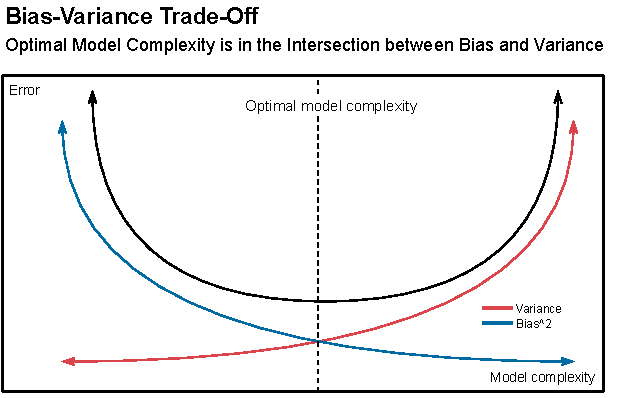
\includegraphics[width=0.8\textwidth]{images/bias-variance.drawio (2).pdf}
    \vspace{1em}
    \caption{{Bias-Variance Trade-Off}}
    \subcaption*{The model complexity is in a trade-off between bias and variance. Here, over-fitting typically entails high bias and low variance, while under-fitting entails low bias and high variance.}
    \label{figure:bias-variance}
\end{figure}

There exist other tree models which can improve the performance of a simple decision tree. Random forest (RF) is one such example, where a "forest" of many decision trees are generated. Here, the prediction made by the final RF model is the average prediction across a single iteration of a single forest. In \autoref{from-decision-tree-to-xgboost} we illustrate a single decision tree model and show the difference between a RF and tree boosting model. Typically, the performance ordering of these are single tree model $<$ RF $<$ tree boosting \parencite{ban404-an-introduction-to-statistical-learning}.  

\begin{figure}[H]
    \centering
    \vspace{1em}
    \begin{subfigure}{0.3\linewidth}
        \centering
        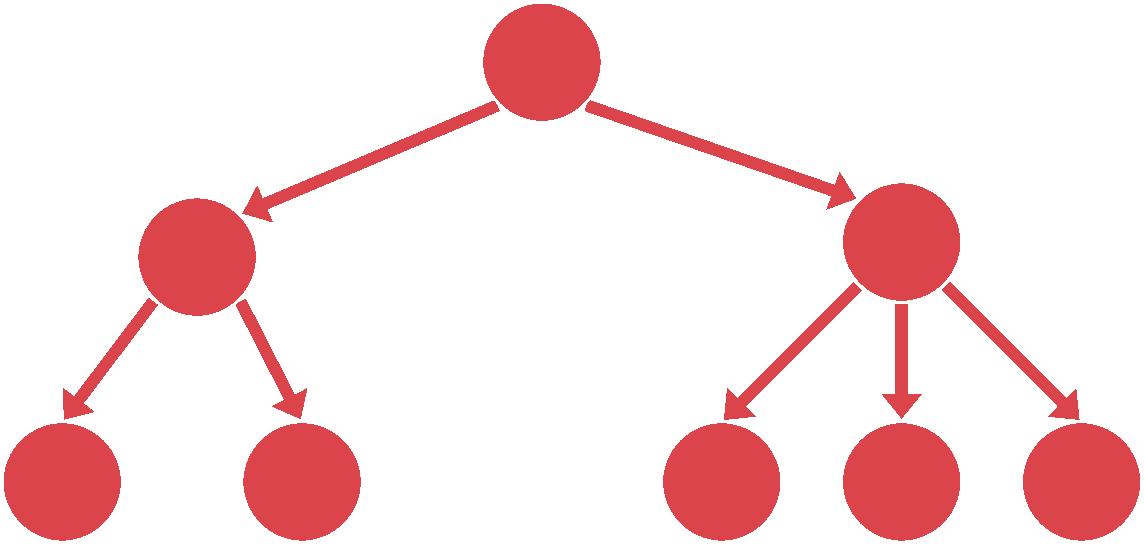
\includegraphics[width=\linewidth, height=\linewidth, keepaspectratio]{images/tree models.drawio.pdf}
        \caption{}
        \label{fig:draw-io-decision-tree}
    \end{subfigure}
    \hfill
    \begin{subfigure}{0.3\linewidth}
        \centering
        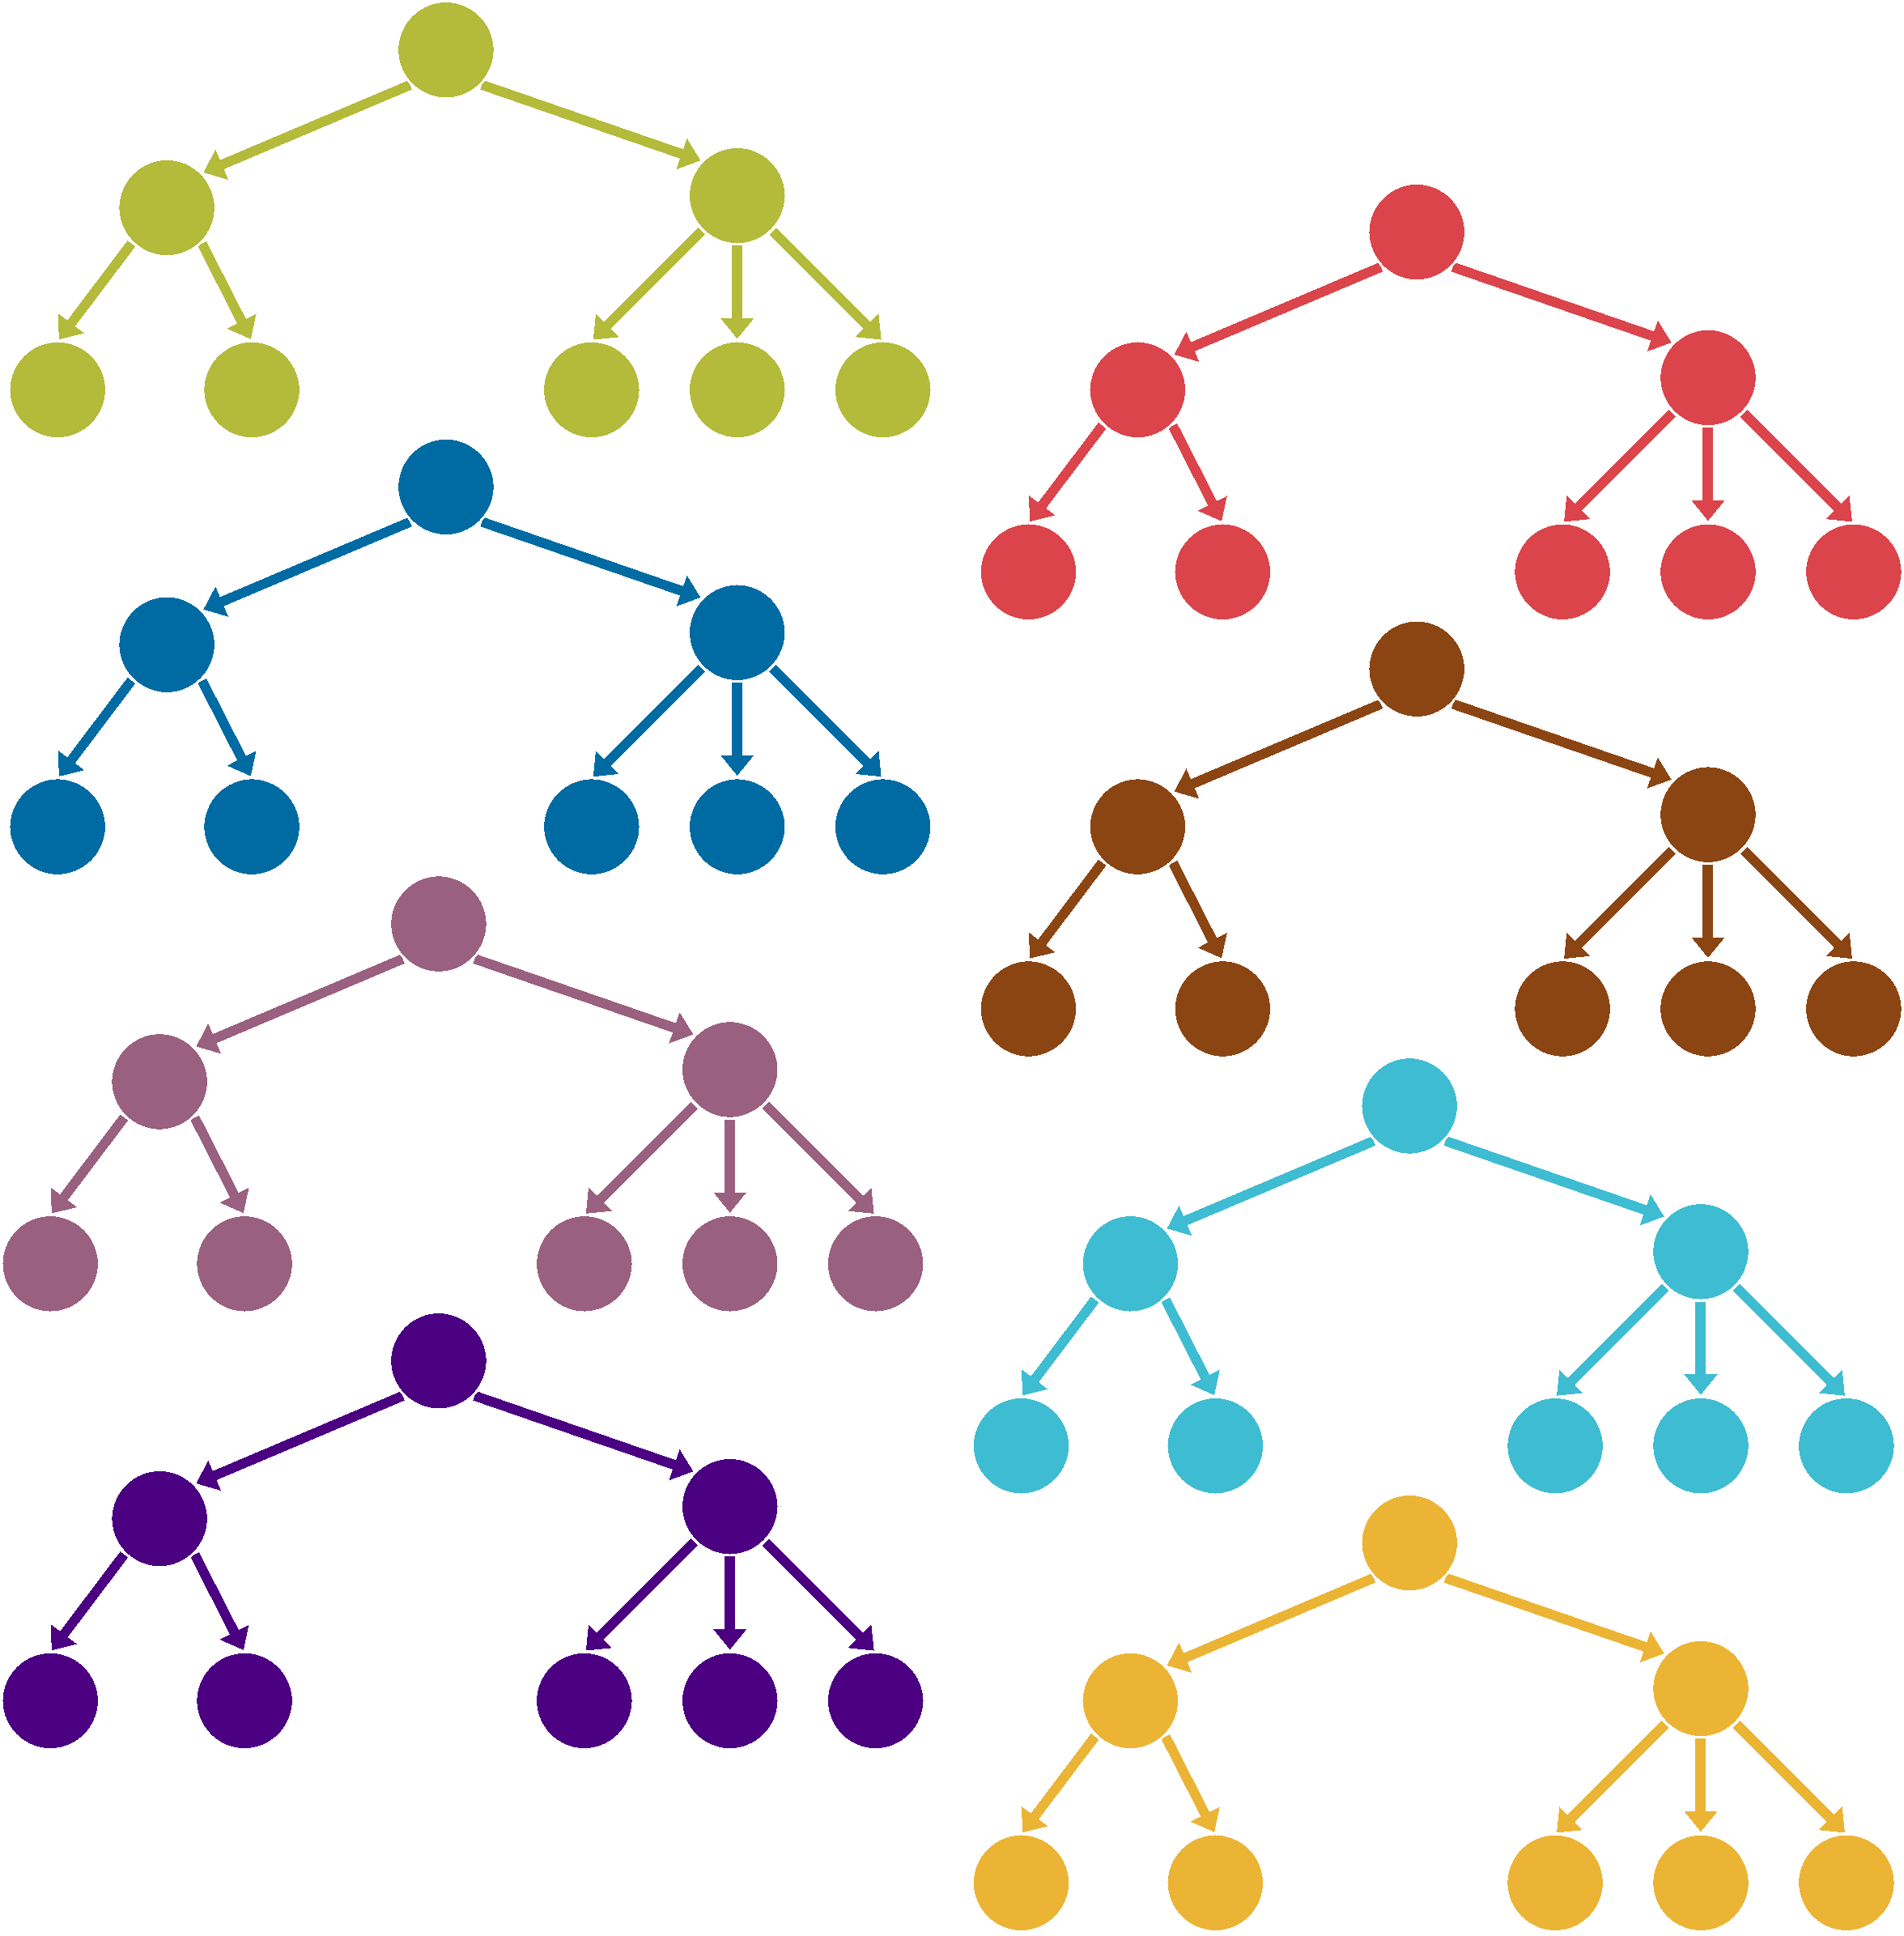
\includegraphics[width=\linewidth, height=\linewidth, keepaspectratio]{images/random forest diagram.drawio.pdf}
        \caption{}
        \label{fig:draw-io-random-forest}
    \end{subfigure}
    \hfill
    \begin{subfigure}{0.3\linewidth}
        \centering
        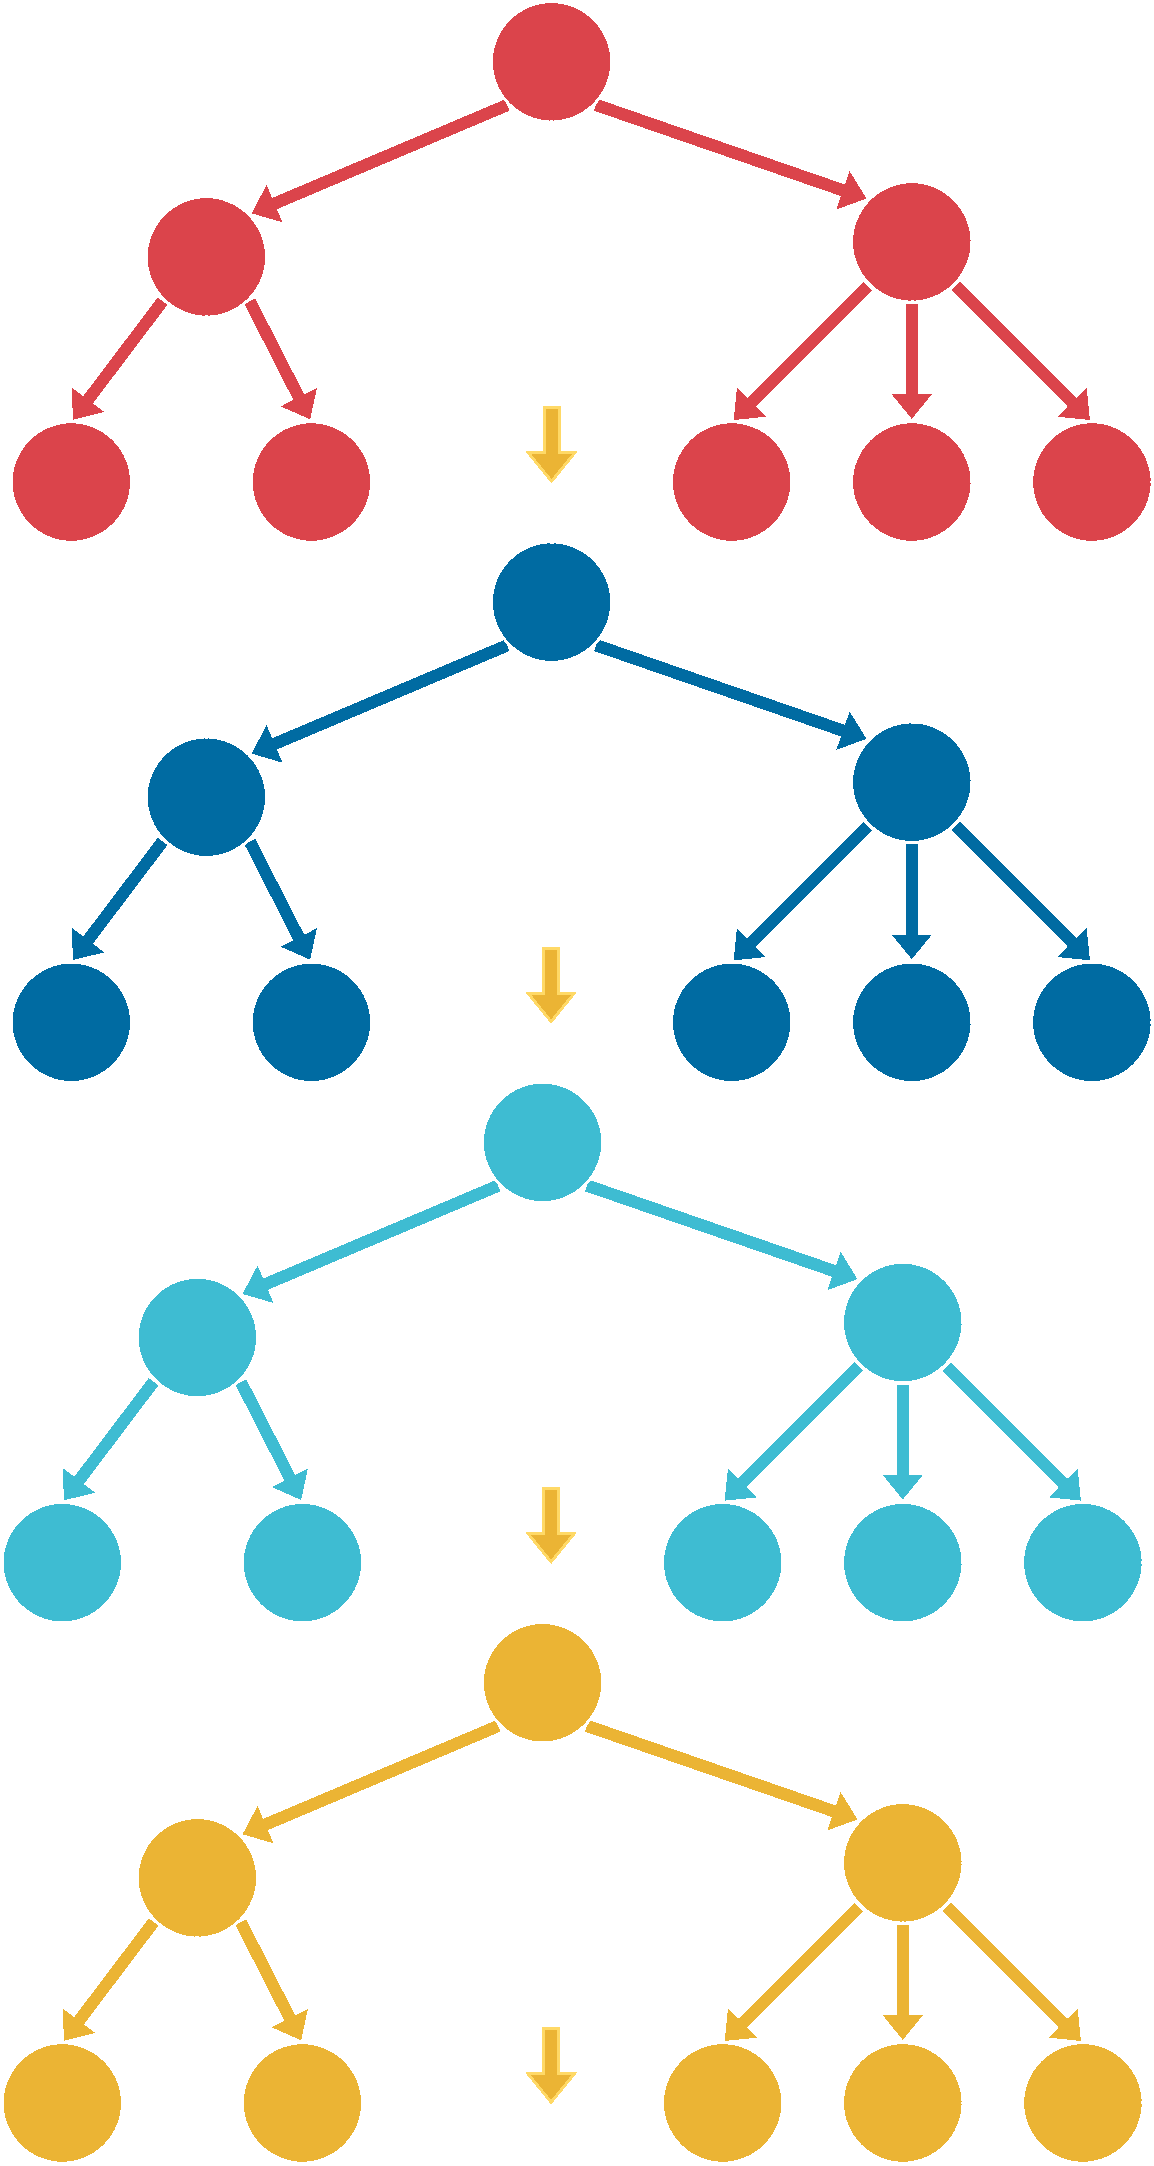
\includegraphics[width=\linewidth, height=\linewidth, keepaspectratio]{images/xgb.drawio.pdf}
        \caption{}
        \label{fig:draw-io-xgboost}
    \end{subfigure}
    \vspace{1em}
    \caption{{From a Single Tree Model (a) to Random Forest (b) to Tree Boosting (c)}}
    \subcaption*{We illustrate the simple intuition behind going from a single decision tree toward more complex tree models. RF average across a single iteration of several trees, while tree boosting aggregate over several iterations of a single tree.}
    \label{from-decision-tree-to-xgboost}
\end{figure}

\subsection{XGBoost}

Following tree-boosting algorithms producing competitive and robust classification models, \textcite{friedman-greedy-function-approximation} introduced gradient boosting. This is based on gradient descent. In other words, gradient boosting seeks to optimise an algorithm by finding the minimum of a function. It does so by moving opposite to the gradient of the function, or steepest ascent. The move from gradient to hessian boosting includes using not only first-order (gradient), but also second-order (hessian) methods when optimising boosting algorithms \parencite{ntnu-thesis-why-does-xgboost-win-every-machine-learning-competition}. XGBoost by \textcite{xgboost-a-scaleable-tree-boosting-system} is a tree boosting model which utilise both gradient and hessian boosting.  

The last years have seen a prominent rise in the popularity of XGBoost, by winning several ML competitions \parencite{ntnu-thesis-why-does-xgboost-win-every-machine-learning-competition}. XGBoost is renowned for its efficiency and flexibility in handling various data types, and the ability to customise XGBoost has made it an optimal tree-boosting system of choice in ML competitions \parencite{ntnu-thesis-why-does-xgboost-win-every-machine-learning-competition}. 

The function \texttt{xgboost::xgboost()} is an application of this in R \parencite{xgboost-package-yuan}. The documentation builds on work by \textcite{friedman-additive-logistic-regression} and \parencite*{friedman-greedy-function-approximation}. XGBoost comes with a wide range of configurable hyperparameters, which can be used to utilise the full potential of the model \parencite{kaggle-xgboost-hyperparameter}. The hyperparameters might be optimised to increase a specific measure, but in our application, we have used a set of parameters without optimising. This is mainly due to the low complexity of our classification problem. Hyperparameters used in this thesis are shown in \autoref{xgb-hyperparameters}.


\subsection{Posterior Probability Threshold}

The ML models output an estimated likelihood of which class the observations belong to, but the actual classification is determined based on the likelihood being above or below a certain threshold. This threshold is often set to 0.5, but in some practical applications, the predictions can be improved by using a different threshold \parencite{ban404-an-introduction-to-statistical-learning}. As \textcite{ban404-an-introduction-to-statistical-learning} mentions, when predicting if a bank customer is going to default or not, one can adjust the threshold to increase accuracy. \textcite{ban404-an-introduction-to-statistical-learning} refer to this threshold as the \textit{posterior probability threshold} (\textit{PPT}). In short, PPT can be adjusted to accommodate for specific use cases and increase accuracy. In this thesis, PPT can influence the distribution of the predicted additions and deletions to OSEBX, and also the total accuracy. In \autoref{Results and discussion}, we carefully consider which PPT should be applied in this thesis.

\subsubsection{Conditional Posterior Probability Threshold}

In our classification problem, it becomes evident that it is difficult for the ML algorithms to capture when a company is added or deleted from OSEBX. This is a practical challenge because we are dependent on predicting additions and deletions to exploit the index effect. We have considered several approaches to cope with this difficulty. First, we considered (1) implementing a custom objective function in the XGBoost application programming interface (API), where XGBoost enables for customising a loss function and a corresponding evaluation measure. The idea here would be to create a custom objective function to penalise model behaviour when not predicting changes. A different approach is to (2) implement a \textit{conditional PPT}, based on the status of the company in the previous period. The second approach considered is fairly easy to implement, and we investigate this approach further.

Seeking to increase the number of predicted changes made by the ML model, we add a lower PPT for companies not currently on the index (potential predicted additions), and a higher PPT for companies currently on the index (potential predicted deletions). To apply this in practice, let $Y_{i,t}$ represent the class for company $i$ at time $t$. Then $Y_{i,t-1}$ represents the class for company $i$ in the previous period $t-1$. By knowing the $Y_{i,t-1}$ for a specific observation, we can use this information to decide which PPT we would like to apply for that specific classification. When $Y_{i,t-1}$ is equal to 1, we know that the company was listed on OSEBX in the previous period. To increase the total number of predicted deletions, we would therefore use a higher PPT for this classification. In contrast, if $Y_{i,t-1}$ is equal to 0, we would like to lower the PPT, because then we would predict more additions to OSEBX. Next, we introduce a parameter $\varepsilon$ which is either added or subtracted from the PPT. We also define $\theta$ as the PPT, and $\theta^\star$ to be the conditional PPT. The conditional PPT can then be expressed as in \autoref{postprocessing}. 

\vspace{-1em}
\begin{equation}
\begin{aligned}
    \theta^\star = \begin{cases}
    \theta + \varepsilon, &  Y_{i, t-1} = 1 \\
    \theta - \varepsilon, &  Y_{i, t-1} = 0
    \end{cases}
\label{postprocessing}
\end{aligned}
\end{equation}

By using this equation, we must also define the valid values for $\theta^\star$, which can be expressed as $0 < \theta^\star < 1$. When classifying the observations, the predicted class $\widehat Y_{i,t}$ is 1 if the estimated probability $p$ is greater than $\theta^\star$, and 0 if $p$ is smaller than $\theta^\star$. To interpret \autoref{postprocessing} in words, we can describe it as the following: To keep staying on OSEBX will require a higher estimated probability, than entering OSEBX will require. Vice versa, to keep staying off OSEBX will require a lower estimated probability, than exiting OSEBX will require. 

However, by using this approach, we encounter some important considerations. First, if a higher number of trades is better at capturing the index effect, why not buy all companies currently not on OSEBX, and sell all companies currently on OSEBX. By doing so, we would be trading all of the approximately 200 constituents on OSEAX. Most likely, the exploited index effect would then be significantly diminished. Another consideration would be to decide whether or not the conditional adjustment parameter $\varepsilon$ should be symmetrical or not in relation to the PPT. More specifically, we need to decide if the same parameter should be applied in both directions (add and subtract the same parameter from the initial PPT). Because we want to analyse the performance of both long and short positions in our simulated portfolios, we find it more appealing to treat both additions and deletions equally. We proceed using a symmetrical addend in this thesis. In practice, we are required to use a numerical value of $\varepsilon$. In \autoref{Results and discussion} we carefully consider which value of $\varepsilon$ to implement in our models.

\subsection{Machine Learning Performance Measures}

\subsubsection{Confusion Matrix}

A confusion matrix is a useful tool in evaluating and visualising a classification model's performance \parencite{caelan-a-bayesian-interpretation-of-the-confusion-matrix}. In a binary task, the confusion matrix is a 2$\times$2 matrix, where TP is the true positive, FP false positive, FN false negative, and TN true negative, as shown in \autoref{fig:confusion-matrix} \parencite{caelan-a-bayesian-interpretation-of-the-confusion-matrix}. 

\begin{figure}[H]
\centering
\[
\begin{bmatrix}
    TN & FN \\
    FP & TP
\end{bmatrix}
\]
\caption{{Confusion Matrix}}
\subcaption*{Illustration of a confusion matrix, displaying TN (true negatives), FN (false negatives), FP (false positives) and TP (true positives)}
\label{fig:confusion-matrix}
\end{figure}



\subsubsection{Accuracy Metrics}

From the confusion matrix in \autoref{fig:confusion-matrix}, we can calculate accuracy, precision, sensitivity, and specificity \parencite{coenen-confusion-matrix}. Accuracy is calculated as the ratio of correct predictions to the total observations (\autoref{equation:accuracy}), precision is the ratio of true positives to all predicted positives (\autoref{equation:precision}), sensitivity is the proportion of actual positives correctly identified (\autoref{equation:sensitivity}), and specificity is the proportion of actual negatives correctly identified (\autoref{equation:specificity}) \parencite{coenen-confusion-matrix}. F-score, illustrated in \autoref{equation:f-score-2}, provides a balanced measure of model performance in classifying data, and is especially useful in situations when considering both FP and FN \parencite{xgboost-performance-analysis-of-classifier-with-missing-data}.  

\begin{equation}
\label{equation:accuracy}
\text{Accuracy} = \frac{TP + TN}{TP + FP + FN + TN} 
\end{equation}
\begin{equation}
\label{equation:precision}
\text{Precision} = \frac{TP}{TP + FP} 
\end{equation}
\begin{equation}
\label{equation:sensitivity}
\text{Sensitivity} = \frac{TP}{TP + FN}
\end{equation}
\begin{equation}
\label{equation:specificity}
\text{Specificity} = \frac{TN}{TN + FP}
\end{equation}
\begin{equation}
\label{equation:f-score-2}
    \text{F-score} = \frac{TP}{TP + \frac{(FP+FN)}{2}}
\end{equation}

\subsubsection{Area Under Receiver Operating Curve}

The receiver operating characteristics (ROC) curve depicts the performance of a classifier in two dimensions, with sensitivity (true positive rate) and 1-specificity (false positive rate) along the axes \parencite{fawcett-an-introduction-to-roc-analysis}. AUROC gives a model performance in the interval from 0 to 1 \parencite{hanley-area-under-a-receiver-operating-curve}. \autoref{fig:area-under-roc-curve-illustration} illustrates AUROC, where 0.5 is a random guess, and 1.0 is a perfect classifier. 

\begin{figure}[H]
    \centering
    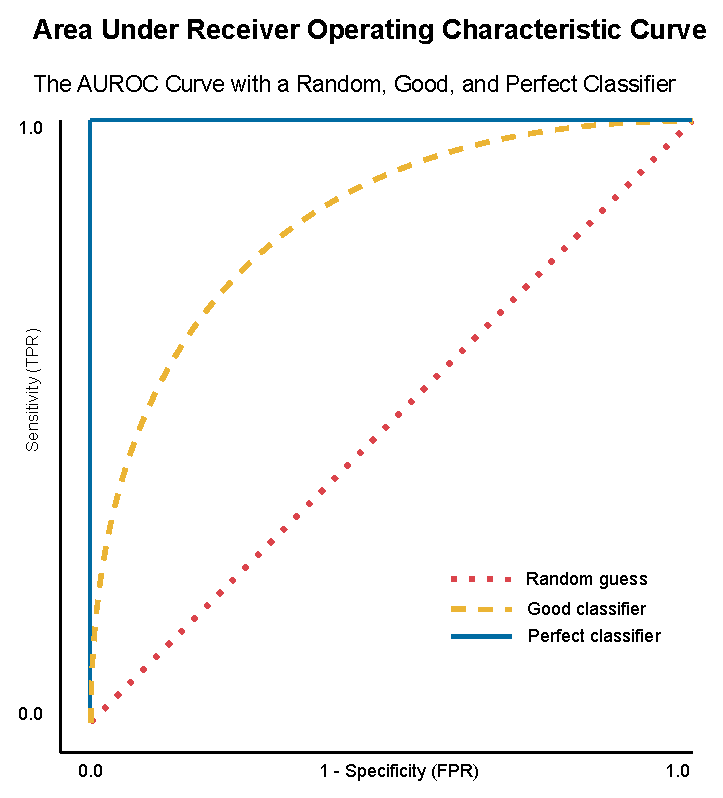
\includegraphics[width=0.45\textwidth]{images/auroc_goodie.drawio (3).pdf}
    \vspace{0.1em}
    \caption{{The AUROC Curve}}
    \subcaption*{The area under receiver operating characteristic curve is shown with a random guess, a good classifier, and a perfect classifier.}
    \label{fig:area-under-roc-curve-illustration}
\end{figure}

\subsubsection{Variable Importance Plot}

ML models have commonly been evaluated with only a single metric, such as accuracy \parencite{koalaverse-varimp}. However, it is increasingly important to not only focus on model predictions but also to understand how these predictions are made \parencite{doshi-velez-interpretable-machine-learning}. VIP shows the relative significance of each predictor variable in an ML model \parencite{koalaverse-varimp}, as shown in \autoref{fig:variable-importance-plot-theory}. VIP is calculated differently across ML models, but the core idea is to display the relative importance of predictor variables \parencite{wei-variable-importance-a-comorehensive-review}. VIP can be applied in R using the \texttt{vip::vip()} function \parencite{vip-documentation}. 

\begin{figure}[H]
    \centering
    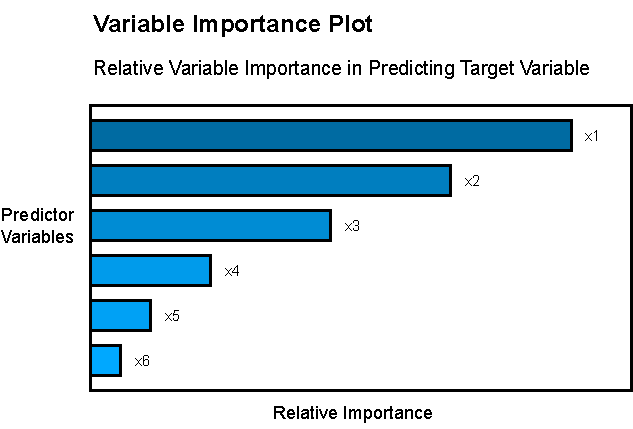
\includegraphics[width=0.6\textwidth]{images/variable-importance.drawio (3).pdf}
    \vspace{1em}
    \caption{{VIP}}
    \subcaption*{This shows the relative importance of predictor variables in predicting the target variable. Note that these are relative metrics, and absolute numbers will deviate between GLM and XGBoost models, as seen in \autoref{Results and discussion}.}
    \label{fig:variable-importance-plot-theory}
\end{figure}

\subsection{Summary of Methodology}

In this section, we first looked at ML and the application of ML methods in finance. We introduced the ML models GLM and XGBoost, where both will be used in the portfolio simulation in \autoref{Results and discussion}.  Further, we also introduced PPT, the conditional PPT, and the ML performance metrics, as summarised in \autoref{tab:methodology-performance-metrics}. For the numeric ranges in \autoref{tab:methodology-performance-metrics}, values closer to 1 are desirable. 

\begin{table}[H]
\centering
\begin{tabularx}{0.5\textwidth}{XX}
\hline
Metric       & Range \\
\hline
Accuracy              & [0, 1] \\
Precision             & [0, 1] \\
Sensitivity           & [0, 1] \\
Specificity           & [0, 1] \\
F-score               & [0, 1] \\
AUROC                 & [0.5, 1] \\
VIP & Relative \\
\hline
\end{tabularx}
\vspace{1em}
\caption{{Summary of ML Evaluation Metrics}}
\subcaption*{In principle we are looking for higher values for the performance metrics accuracy, precision, sensitivity, specificity, F-score, and AUROC. In \autoref{Results and discussion} we will discuss how only looking at accuracy measures may be misleading depending on the practical application of an ML model.}
\label{tab:methodology-performance-metrics}
\end{table}


\newpage
\section{Data}\label{Data}

\subsection{Introduction to Data}

The Euronext index methodology for OSEBX lays the foundation of data used in our analysis \parencite{OSEBX-rule-book}. Euronext collects data on OSEAX companies on CD, which are used to calculate upcoming index composition. The compositions are publicly announced on AD, and implemented on ED \parencite*{OSEBX-rule-book}, as shown in \autoref{fig:timeline-index-rebalancing}. For OSEBX, this timeline occurs twice a year, as the benchmark index rebalances semi-annually in March and September \parencite*{oslo-stock-exchange-news-web}. In \autoref{Results and discussion}, we use data from January 2006 to March 2023.

We decided to analyse three different prediction horizons so that for each index rebalancing event, we collect data from 30, 60, and 100 business days before ED. For example, for the index rebalancing event in March 2023, where ED is 2023-03-17, we collect data for all OSEAX companies in February of 2023, December and October of 2022. 

\begin{figure}[ht]
    \centering
    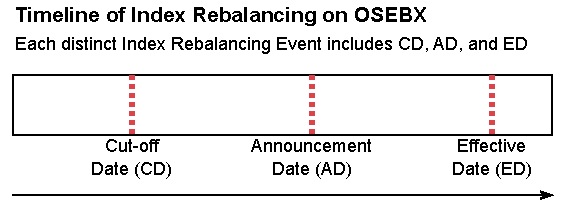
\includegraphics[width=0.8\linewidth]{images/timeline-cd-ad-ed.drawio (4).pdf}
    \vspace{1em}
    \caption{{OSEBX Index Rebalancing Timeline}}
    \subcaption*{Timeline of a single index rebalancing event on OSEBX with CD, AD, and ED. In the portfolio simulation in \autoref{Results and discussion} from 2010 to 2023 we experienced two distinct index rebalancing events each year (except 2020).}
    \label{fig:timeline-index-rebalancing}
\end{figure}

\subsection{Variables}

Euronext collects four key variables on CD reflecting the liquidity and size of companies \parencite{oslo-stock-exchange-news-web}. The first variable explains the proportion of a company's active trading days out of the total trading days in a given period \parencite*{OSEBX-rule-book}. We call this variable \texttt{trading\_status}. The second is turnover (electronic order book), which is the total value of shares traded at the end of the last 12 months up to and including CD, but excluding the 12 days with the highest turnover for each company \parencite*{OSEBX-rule-book}. We name this variable \texttt{turnover\_eob}. The next variable is the free float factor, which represents the free float market capitalisation for the total market value of shares that are publicly available for trading \parencite*{OSEBX-rule-book}. We call this variable \texttt{free\_float}. The last collected financial variable \texttt{icb\_supersector} is based on the industry classification benchmark (ICB) according to Dow Jones and FTSE \parencite{industry-classification-benchmark}. 

In short, Euronext collects the four variables above to calculate index composition, based on the publicly available index methodology \parencite{OSEBX-rule-book}. We do not review the rule book in greater detail here but in general the bigger \texttt{turnover\_eob}, \texttt{free\_float} and \texttt{trading\_status}, the more likely the company will be included on OSEBX according to \textcite{OSEBX-rule-book}. In this thesis, we seek to use the variables Euronext collects and use ML to predict upcoming index composition \textit{before} AD. If we can predict OSEBX changes before they are announced to the public, we may gain a temporal advantage. We seek to make our ML models as simple as possible, and therefore try not to use additional financial variables, which are not mentioned in the OSEBX rule book \parencite{OSEBX-rule-book}. We consider our findings to be easier to replicate and understand when not using any additional financial variables.


\subsubsection{Target Variable}

In our data, we introduce the binary target variable \texttt{index\_cp} to denote if a company is on the benchmark index OSEBX in the current period. This variable is equivalent to $Y_{i,t}$ explained in \autoref{Methodology}. The current period represents the time from the last ED to the upcoming ED. As such, we seek to predict \texttt{index\_cp} for the \textit{next} period. The binary target variable \texttt{index\_cp} is 1 if the company is on OSEBX, and 0 otherwise. Labeling our data set as such becomes an ML classification problem using SL \parencite{ban404-the-elements-of-statistical-learning}.

\subsubsection{Lag Variables}

 Certain selection criteria differ for companies being on/not on OSEBX \parencite{OSEBX-rule-book}. Furthermore, we are dependent on knowing the lagged target variable to use the conditional PPT, introduced in \autoref{Methodology}, where the lagged variable is denoted as $Y_{i, t-1}$. Therefore, we introduce lag variables showing the binary value for \texttt{index\_cp} in the previous periods. We introduce lag variables \texttt{index\_lag1}, \texttt{index\_lag2}, \texttt{index\_lag3}, and \texttt{index\_lag4} for the value of \texttt{index\_cp} in the previous 1 to 4 periods. Lag variables can be applied in R with the \texttt{stats::lag()} function \parencite{lag-variable-R}. 


\subsection{Data Sources}

We first collect the dates for relevant index rebalancing events from \textcite{oslo-stock-exchange-news-web}. Thereafter, we collect the benchmark index constituents on OSEAX and OSEBX the day after each ED, to make sure we know the index composition \textit{just after} each rebalancing event. Further, we collect the four financial variables for each company 30, 60, and 100 days in advance of the ED. This is done using a Bloomberg Terminal (BBG) \parencite{bloomberg-terminal}. For the portfolio simulation, we obtain stock prices for all companies using DataStream and a Refinitiv Terminal \parencite{nhh-data-stream}. Lastly, we obtain FF3 data by \textcite{bernt-fama-french}. 

We find public announcements on OSEBX constituents by \textcite{oslo-stock-exchange-news-web} dating back to 2002. In both the BBG and Refinitiv Terminals we are able to find variable and price data for some companies backdating to 2002, but also find significant missing values for other companies in the period before 2006. With this backdrop, we conclude to use data from January 2006 to March 2023, which after data manipulation yields a clean data set with no NA-values. The selected time horizon gives a total of two distinct index rebalancing events each year (except for 2020 when Euronext changed from rebalancing in June/December to March/September), all including a CD, AD, and ED, with the first and last ED being 2006-06-30 and 2023-03-17. All rebalancing dates (CD, AD, and ED for each rebalancing) are shown in \autoref{APPENDIX CD, AD, and ED from 2006 to 2023}.

\subsubsection{Bloomberg}

Specifically, we obtain data from BBG through the BBG Query Language (BQL) \parencite{bloomberg-professional-services-BQL}, implemented in Excel \parencite{BQL-fintools}. We retrieve historical data points through functions such as \texttt{BDH}, \texttt{BDP}, and \texttt{BQL} \parencite{dartmouth-BQL}. Please note that the specific BQL functions used are shown in \autoref{APPENDIX-Excel-Bloomberg-Add-In-BQL-Formulas}. In conclusion, after gathering data from BBG we were left with a data frame, including the following variables \texttt{DD} (the date the data was collected, 30, 60 or 100 days in advance of ED), \texttt{CD}, \texttt{AD}, \texttt{ED}, \texttt{ticker}, \texttt{name}, \texttt{icb\_supersector}, \texttt{free\_float}, \texttt{turnover\_eob},  \texttt{trading\_status} and \texttt{index\_cp}. Please note that \texttt{index\_cp} is defined as 1 if the observation's combination of ticker and ED exists in the data frame where only the OSEBX constituents are stored, which we also obtained from BBG. These variables are collected for each company listed on OSEAX since 2006.


\subsubsection{DataStream}
Because we want to simulate the historical performance of the constructed portfolios, we need to collect historical price data. In the simulations, we use volume-weighted average price (VWAP). The VWAP is a more accurate representation of the share price we could have bought or sold many stocks for, compared to the closing price (which is often reported when illustrating stock price development). VWAP is also commonly used to evaluate the performance of stock traders \parencite{madhavan-vwap}. The VWAP is collected using Refinitiv DataStream of all OSEAX companies in the period from 2006 to 2023 \parencite{nhh-data-stream}. Collecting these prices is done in practice through the Refinitiv terminal \parencite{lseg-refinitiv}, with an Excel add-in \parencite{refinitiv-excel-add-in}. The data frame generated by DataStream consists of one date column, and 487 columns representing each company to ever be listed on OSEAX since 2006. In conclusion, this data source gives us the historical VWAP for each company for each day since 2006.


\subsubsection{Fama-French 3-factor Model Data}

The FF3 factors on Oslo Stock Exchange (OSE), such as sensitivity to size $\beta_{i,SMB}$ and $\beta_{i,HML}$ is collected from a data file compiled by \textcite{bernt-fama-french}. Note that the collected FF3 is only available until 2022-05-31. As such, the actual portfolio simulation in \autoref{Results and discussion} goes until 2023-03-17, but the portfolio performance assessments use the period from 2010-02-28 to 2022-05-31 due to lack of FF3-factors after May of 2022.

\subsubsection{Risk-Free Interest Rate}

The risk-free interest rate $R_f$ is the expected return on a zero-risk investment, introduced by \textcite{irving-theory-of-interest}. It is useful when calculating the financial metrics discussed in \autoref{Theoretical background}. The risk-free rates $R_f$ in the Norwegian market are estimated and published by \textcite{bernt-risk-free}. We collect the monthly risk-free rate $R_f$ from \textcite{bernt-risk-free}, for the portfolio performance analysis period from 2010 to 2023. Thereafter we average these rates, which amounts to a monthly risk-free rate of $\approx$ 0.12\%, or 1.46\% annually. 

\subsection{Data Manipulation and Missing Data}
After obtaining the data presented, we still need to make certain operations to make it viable for analysis. We are now referring to the data set obtained from BBG, which ultimately is what will be used for our analysis. When a company is listed on OSEAX after the data cutoff point, we receive NA-values for those companies for the relevant period. This makes it somehow difficult to capture for our ML model if company data is not available at or before CD (or the date of prediction). Vice versa, it is difficult if a company is unlisted from OSEAX between CD and ED. We simply decide to remove rows where data on CD is not available, as this has minimal influence on our data set, and most of the companies entering OSEAX are not eligible for OSEBX the same period, with some exceptions, \parencite{OSEBX-rule-book}.

Regarding \texttt{icb\_supersector}, we are missing this variable for some companies before 2010. This stems from companies being classified before the standardisation toward ICB and then delisted. Luckily, we find the Global Industry Classification Standard (GICS) for these companies \parencite{global-industry-classification-standard}. Because ICB and GICS overlap, with 25 and 20 level 2 classifications each, we choose to manually estimate ICB for the relevant companies, as shown in \autoref{APPENDIX From GICS to ICB}. 

After cleaning the data sets for NA-values, we add the lagged variables \texttt{index\_lag1}, \texttt{index\_lag2}, \texttt{index\_lag3}, and \texttt{index\_lag4} using the \texttt{stats::lag()} function \parencite{lag-variable-R} in R. 

\subsection{Train-Test Split}

Splitting the data set into train and test data is an approach used in cross-validating ML models \parencite{geisser-cross-validation}. The idea of cross-validation is that the accuracy of the ML model is evaluated on a data set (test data), that is different than the data set it is trained on (train data). The approach is used to avoid over-fitting, as the test data set is not leaked to the train data set. To create a train-test split in our case, we use time series cross-validation (TSCV) \parencite{bergmeir-time-series-cross-validation}. Here we train the models on all historical rebalancing events before the point in time the predictions are made. Originally, we start by using train data up to before 2010, and thereafter add one period of train data for each new index rebalancing event. \autoref{fig:train-test-split} illustrates the split between the train and test data set we use in TSCV. As an example, when making predictions leading up to March of 2023 in \autoref{fig:train-test-split}, we train the ML model on all data up to that point. 

\begin{figure}[H]
    \centering
    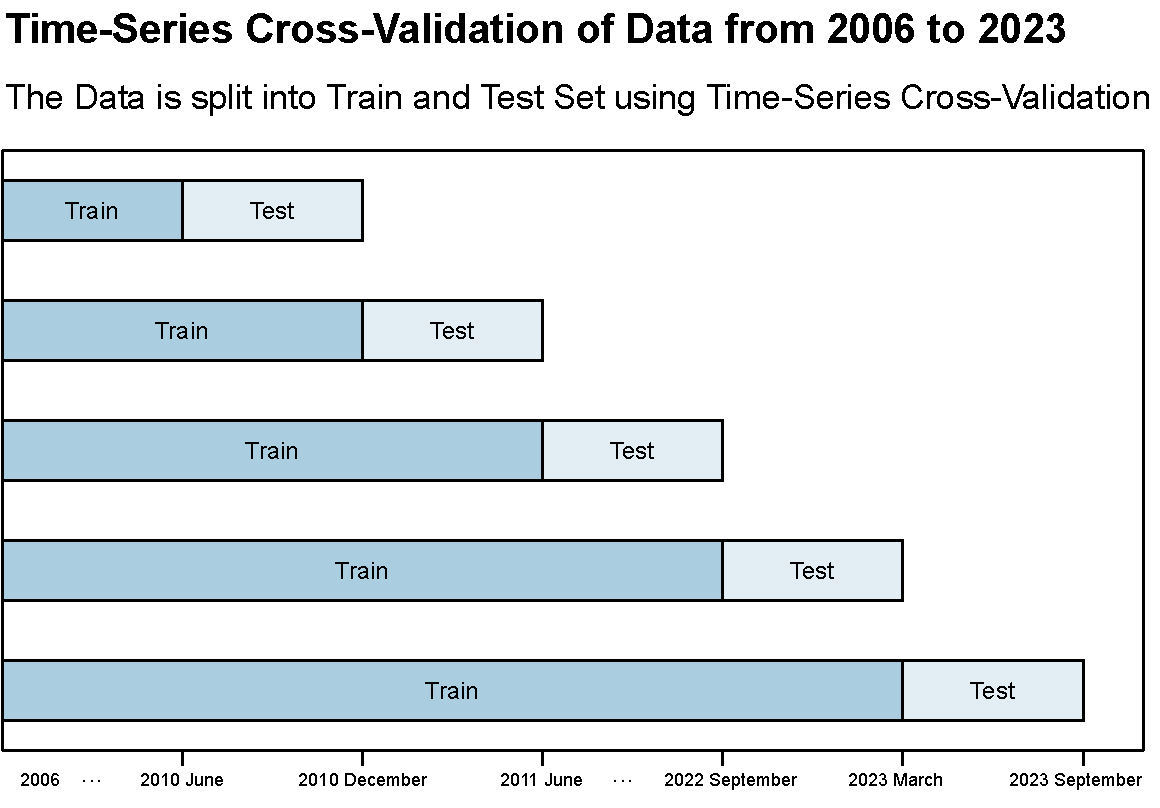
\includegraphics[width=0.8\textwidth]{images/train-test-split.drawio (4).pdf}
    \vspace{1em}
    \caption{{Time Series Cross-Validation}}
    \subcaption*{TSCV used in portfolio simulation for the trading strategy and enhanced index investing strategy.}
    \label{fig:train-test-split}
\end{figure}

\subsection{Summary of Data}

The final data set used in the ML models is summarised in \autoref{tab:final-data-set-predictor-target}. In short, we have generated three data sets containing these variables, one data set per prediction horizon of 30, 60, and 100 days before ED. As such, the \texttt{trading\_status}, \texttt{turnover\_eob} and \texttt{free\_float} will be somewhat different between the three data sets. The lagged variables from \texttt{index\_lag1} to \texttt{index\_lag4} will be the same across prediction horizons, as the time horizons of 30, 60, and 100 days do not overflow to the previous period. Note that \texttt{index\_cp} is the target variable, which after prediction indicates if the company will be or not be on OSEBX in the \textit{next} period. The lag variable \texttt{index\_lag1} indicates if a company is on OSEBX before the upcoming index rebalancing event. Also note that we use all the predictor variables in \autoref{tab:final-data-set-predictor-target} when predicting the target variable \texttt{index\_cp}. One could probably investigate further if all variables are necessary, and maybe even add other financial variables indicating size and liquidity. In short, we have chosen to keep the number of predictor variables relatively small compared to the amount of data points. The number of rows in the data sets is 5983, 5924, and 5891 for the 30, 60, and 100-day data frames respectively. The difference in the number of rows comes from the fast listings/delistings problem which means we need to discard more rows the longer the prediction horizon.



\begin{table}[H]
\centering
\begin{tabularx}{0.8\textwidth}{lXl}
\toprule
Variables & Explanation & Abbreviation \\ 
\midrule
{Informational variables:} \\
\texttt{data\_date}         & Data Date  & \texttt{DD} \\
\texttt{cutoff\_date}       & Cut-off Date  & \texttt{CD} \\
\texttt{announcement\_date} & Announcement Date & \texttt{AD} \\
\texttt{effective\_date}    & Effective Date & \texttt{ED} \\
\texttt{ticker}             & BBG Ticker \\
 & \\
{Predictor variables:} \\
\texttt{trading\_status}    & Share of Days Traded   & \texttt{TS}\\
\texttt{turnover\_eob}      & Turnover & \texttt{TO}\\
\texttt{icb\_supersector}   & ICB  & \texttt{ICB}\\
\texttt{free\_float}        & Free Float Market Cap & \texttt{FF} \\
\texttt{index\_lag1}        & \texttt{lag(index\_cp,1)} & \texttt{L1} \\
\texttt{index\_lag2}        & \texttt{lag(index\_cp,2)} & \texttt{L2} \\
\texttt{index\_lag3}        & \texttt{lag(index\_cp,3)} & \texttt{L3} \\
\texttt{index\_lag4}        & \texttt{lag(index\_cp,4)} & \texttt{L4} \\
 & \\
{Target variable:} \\
\texttt{index\_cp} & {1 if on OSEBX, 0 otherwise} &  \texttt{IC} \\
\bottomrule
\end{tabularx}
\vspace{1em}
\caption{{The Final Data Set of Predictor Variables and Target Variable}}
\subcaption*{Predictor Variables used in the ML models to predict the target variable \texttt{index\_cp} for the next period. Informational variables are from OSE Newsweb, financial predictor variables are from Euronext index methodology for OSEBX and lagged predictor variables are calculated.}
\label{tab:final-data-set-predictor-target}
\end{table}

Before we present our results, we briefly present a descriptive plot to better understand the data set. The number of listed companies on OSEAX and OSEBX is illustrated in \autoref{Members over time}, and we note that there are approximately 50$-$80 members on OSEBX for a given period, significantly less than those companies not included on OSEBX. There seem to be only about 5$-$10 additions and deletions in total for each period, as shown in \autoref{fig-OSEBX-Number-of-Additions-and-Deletions}.
\begin{figure}[H]
    \centering
    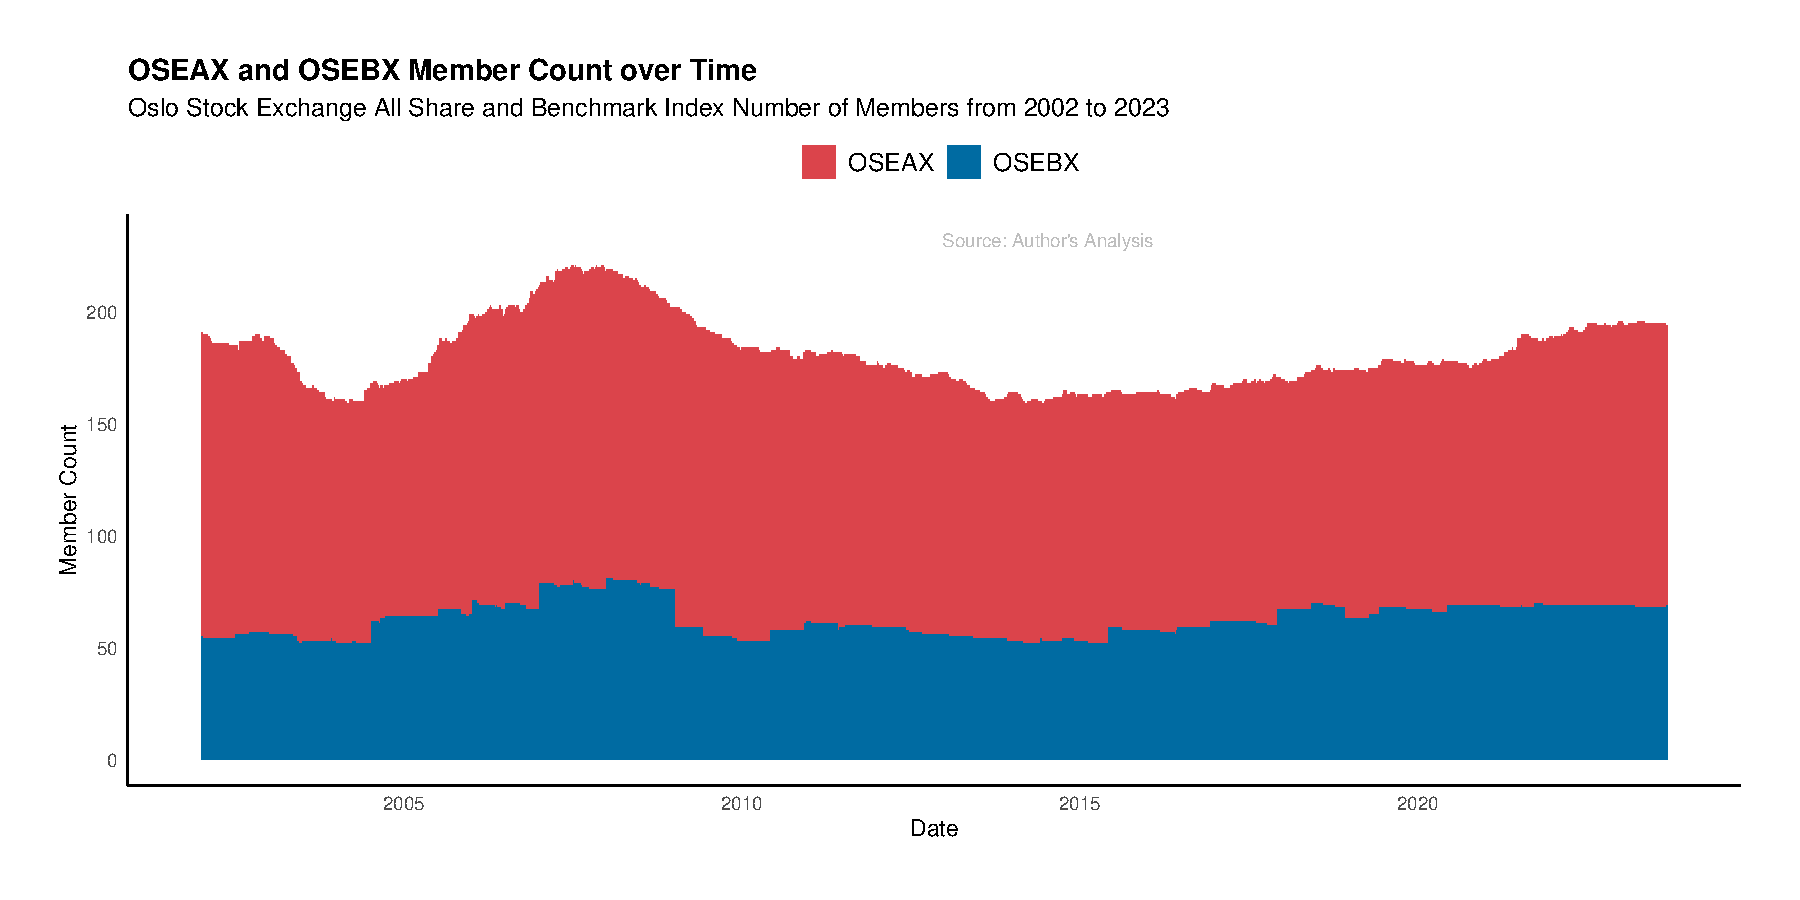
\includegraphics[width=\textwidth]{images/plotmemb_correct.pdf}
    \caption{{Members over Time}}
    \subcaption*{All OSEBX companies are also on OSEAX. Notice that OSEAX typically has about 200 companies, whereas 50-80 companies on OSEBX.}
    \label{Members over time}
\end{figure}










\newpage
\section{Results and Discussion}
\label{Results and discussion}
% \setcounter{equation}{0}

\subsection{Introduction to Results and Discussion}

In this section we first assess the model accuracy of our predictive ML models, using metrics as described in \autoref{Methodology}, and summarised in \autoref{tab:methodology-performance-metrics}. This seeks to answer the first research question (1) "To what degree can machine learning algorithms predict the index composition of OSEBX in the next period?". Next, we simulate portfolios in an active trading strategy, where we trade on the predicted additions and deletions made by the ML models. We do so by running a portfolio simulation from 2006 to 2023 and assessing the performance with financial metrics introduced in \autoref{Theoretical background}. This seeks to answer the second research question (2) "To what degree can trading on predicted additions and deletions outperform OSEBX in an active trading portfolio?". Lastly, we repeat the portfolio simulation, but this time in an enhanced index strategy, seeking to answer research question (3) "To what degree can trading on predicted additions and deletions outperform OSEBX in an enhanced index portfolio?"

\subsubsection{Preliminary Machine Learning Models Summary}

We apply logistic regression using GLM, and tree boosting using XGBoost. In XGBoost we use a standard benchmark model (XGBoost benchmark). We also use an XGBoost model with conditional PPT (XGBoost custom). For each index rebalancing event, we predict either 30, 60, or 100 days prior to ED, all of which happens \textit{before} AD. This is indicated in the suffix of the model names, as summarised in \autoref{tab:machine-learning-model-names}. In total, we are analysing nine unique models. All hyperparameters used in the XGBoost-models are summaries in \autoref{xgb-hyperparameters}. 



\begin{table}[H]
\centering
\footnotesize
\begin{tabularx}{\textwidth}{lXXX}
\hline
Model                    & ED-30     & ED-60     & ED-100 \\
\hline
GLM                     & GLM30     & GLM60     & GLM100 \\
XGBoost Benchmark       & XGBB30    & XGBB60    & XGBB100 \\
XGBoost Custom          & XGBC30    & XGBC60    & XGBC100 \\
\hline
\end{tabularx}
\vspace{1em}
\caption{{ML Model Names}}
\subcaption*{Overview of ML-models used. We predict using logistic regression (GLM), XGBoost benchmark (XGBB) and XGBoost with conditional PPT (XGBC). For each of these models, we predict 30, 60, and 100 days before ED, which correspond to the model names.}
\label{tab:machine-learning-model-names}
\end{table}

\subsubsection{Posterior Probability Threshold Applied}

To determine which PPT to apply, we experimented with different thresholds on the models to better understand the direction of the accuracy when changing the threshold. The models seem to be pruned towards predicting more FP and TP classifications compared to FN and TN. Our models are able to correctly predict more additions than deletions, which according to \autoref{fig:index-effect-osebx} might be sub-optimal. \autoref{fig:index-effect-osebx} illustrate that taking short positions on deletions might have higher expected returns than taking long positions on additions. Therefore, we tweaked the PPT slightly upwards. This gave us higher overall accuracy and a more evenly distributed allocation between additions and deletions. In \autoref{tab:glm_accuracy} we show the tweaking of PPT compared to the predictive accuracy for the model GLM30. Here, we choose to illustrate PPT for GLM30, but in general, the other models show a similar pattern as shown for the GLM30 model. 
\vspace{2em}
\begin{table}[H]
\centering
\begin{tabular}{llllllll}
  \hline
Threshold & 0.3 & 0.4 & 0.5 & 0.6 & 0.7 & 0.8& 0.9  \\
\midrule
Accuracy & 0.9394 & 0.9464 & 0.9471 & 0.9482 & 0.9452 & 0.9407 & 0.9149\\
   \hline
\end{tabular}
\vspace{1em}
\caption{{Tuning PPT for ML models}}
\subcaption*{This illustrates the accuracy in relation to PPT for the GLM30 model. We find this model to be somewhat representative, and choose to set PPT for all models to 0.6.}
\label{tab:glm_accuracy}
\end{table}

We therefore continue using 0.6 as our initial PPT in the models, but we are yet to determine the $\varepsilon$ parameter to be applied in XGBoost custom models (where we use the conditional PPT). To understand how the number of predicted changes behave when changing the $\varepsilon$ parameter, we illustrated this relationship in \autoref{fig:beta_plot}, fitted to an XGBoost model making predictions 30 days in advance ED. We point out that the total number of predicted changes is the sum of all predicted changes from 2010 and onward.

\begin{figure}[H]
    \centering
    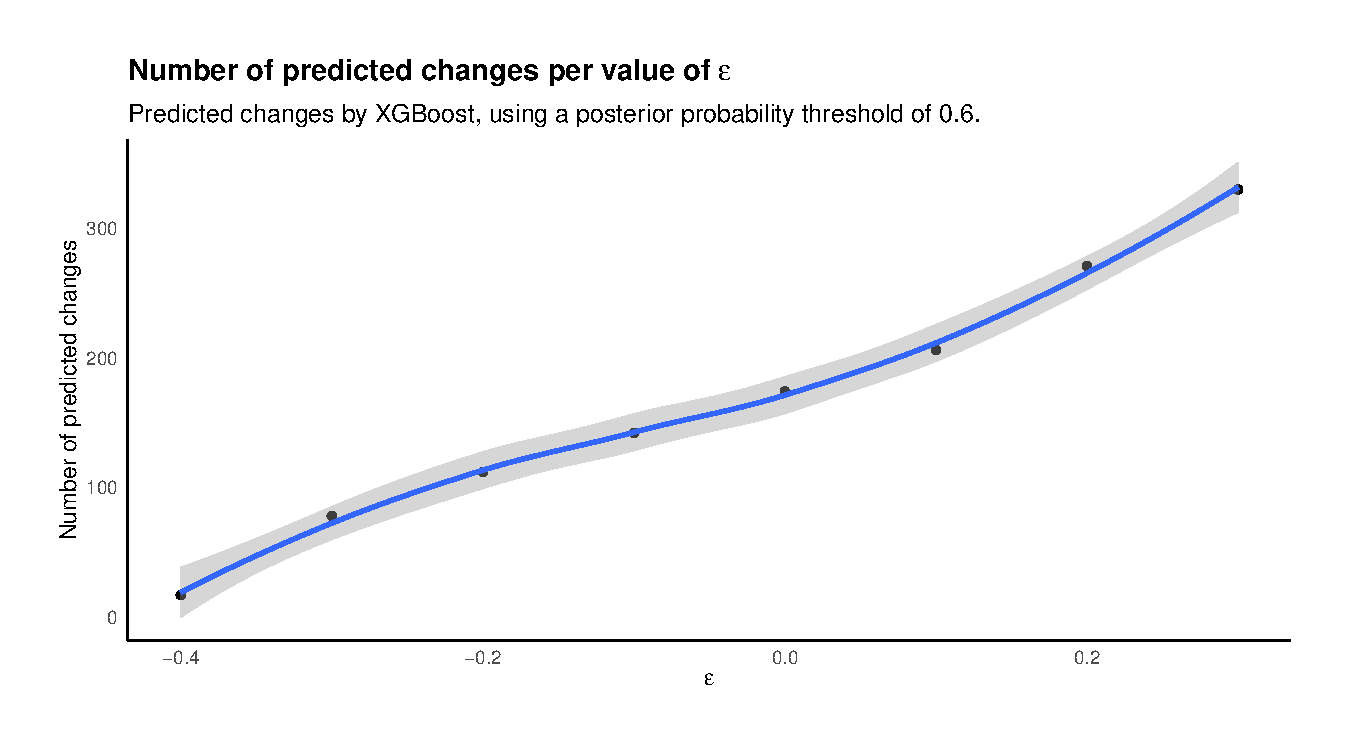
\includegraphics[width=1\textwidth]{images/beta_plot.pdf}
    \caption{{Number of Predicted Changes for Values of $\varepsilon$}}
    \subcaption*{Sum of predicted additions and deletions as a function of $\varepsilon$ in the interval -0.4 to 0.3. Higher $\varepsilon$ correspond to increasing the total number of predicted changes. $\varepsilon$ represents the parameter added or subtracted from the initial PPT, which is fitted to 0.6. In this plot we used an XGBoost model, predicting 30 days ahead of ED.}
    \label{fig:beta_plot}
\end{figure}

\autoref{fig:beta_plot} shows the interval of $\varepsilon$ between -0.4 and 0.3. If we had gone with an even smaller $\varepsilon$, to say -0.6, we would not have gotten any predictions at all. Vice versa, if we had used a $\varepsilon$ of 0.4, we would have gotten $\approx$ 2000 predicted changes. We discarded those cases from the plot to make it easier to read, and because they are irrelevant to our application. 

To decide which $\varepsilon$ to use going forward, we considered different aspects. First of all, we point out that our latter two research questions seek to find out to what degree we can exploit the index effect. The idea of using a conditional PPT is to lower the systematic financial risk and increase the likelihood of buying/selling companies that will be included/excluded from OSEBX. Therefore, we are interested in using a $\varepsilon$ that is higher than 0, because ultimately, we want to increase the number of trades. When $\varepsilon$ is 0, we get the same predictions for XGBoost custom as the XGBoost benchmark model gives, which is a total of about 170 changes. By increasing $\varepsilon$ to 0.2 we predict $\approx$ 270 changes, meaning that the portfolios will be significantly more diversified and eliminating more systematic risk than the portfolios using XGB benchmark and GLM. As we would still like to keep accuracy at an acceptable level compared to the other models, we do not aim to extend the $\varepsilon$ too far and proceed using 0.2 as our $\varepsilon$ parameter in the custom XGBoost models. We would also like to point out that we could have implemented a similar conditional PPT for the GLM models, but we decided to proceed by applying it to the XGBoost models only because they initially are more pruned towards predicting changes than GLM. In practice, the GLM models would require much higher values of $\varepsilon$, and it proved to be more difficult to fit. To conclude this discussion, we proceed using 0.6 as our initial PPT for GLM and XGBB models, and 0.6 $+$/$-$ 0.2 as the conditional PPT for XGBC models.

% RESEARCH QUESTION 1 %%%%%%%%%%%%%%%%%%%%%%%%%%%%%%%%%%%%%%%%%%%%%%%%%%%

\subsection{Research Question (1): To what degree can machine learning algorithms predict the index composition of OSEBX in the next period?}

\subsubsection{Model Accuracy}

In \autoref{confusion_matrix_result} we have illustrated the confusion matrices for the classifications for each model in \autoref{tab:machine-learning-model-names}. 
\begin{table}[H]
\centering
\begin{tabular}{lcccc}
& & GLM & XGBB & XGBC \\
\vspace{1em}
&30 & $\begin{bmatrix} 2729   & 117 \\ 112  & 1462 \end{bmatrix}$ & 
    $\begin{bmatrix} 2683     &  108 \\ 158  &  1471 \end{bmatrix}$ & 
    $\begin{bmatrix} 2639     & 125  \\ 202    &  1454 \end{bmatrix}$\\
\vspace{1em}
$\begin{bmatrix} TN   & FN  \\ FP   &  TP \end{bmatrix}$ & 60 & $\begin{bmatrix} 2711   & 111  \\ 110   &  1458 \end{bmatrix}$ & 
    $\begin{bmatrix} 2666      & 105  \\ 155  &  1464 \end{bmatrix}$ & 
    $\begin{bmatrix} 2628       &  107 \\ 193    & 1462  \end{bmatrix}$  \\
\vspace{1em}
&100 & $\begin{bmatrix} 2698     &  111 \\ 105    &1457  \end{bmatrix}$ & 
     $\begin{bmatrix} 2646   & 114 \\157    & 1454  \end{bmatrix}$ & 
     $\begin{bmatrix} 2605     & 123 \\ 198    &1445  \end{bmatrix}$ \\

\end{tabular}
\vspace{1em}
\caption{{Confusion matrices for all models}}
\subcaption*{The figure shows the confusion matrices for the different models. TN = true negative (we predicted the company not be included on OSEBX, and it did not), FN = false negative (we predicted the company not be included on OSEBX, but it did) FP = false positive (we predicted the company to be included on OSEBX, but it did not) and TP = true positive (we predicted the company to be included on OSEBX, and it did). The matrices show the sum of all rebalancing events since 2010.}
\label{confusion_matrix_result}
\end{table}

First of all, we notice that the models are predicting more TNs than TPs. This is of course as expected, as only 50-80 of the $\approx$ 200 companies on OSEAX are also included on OSEBX. More interestingly, we observe quite evenly matched allocations between FP and FN classifications for the GLM models, meaning that those models are relatively equal in falsely predicting \texttt{index\_cp} = 1 and falsely predicting \texttt{index\_cp} = 0. For the XGBoost models, there are still some imbalances when it comes to allocation between FP and FN, meaning that XGBoost-models are pruned towards predicting more falsely \texttt{index\_cp} = 1 than \texttt{index\_cp} = 0. This can mean that an even higher PPT would even those out, but as our tuning of the PPT showed, that can ultimately decrease overall accuracy. Further, the statistics from the confusion matrices are shown in \autoref{table:accuracy-precision-sensitivity-specificity-f-score}.

\begin{table}[ht]
\centering
\begin{tabular}{llllllll}
  \toprule
Model & Accuracy & Precision & Sensitivity & Specificity & F-score & AUROC & n \\ 
  \midrule
index\_lag1 & 0.9507 & 0.9208 & 0.9399 & 0.9565 & 0.9303  & 0.9446 & 0 \\
  \midrule
GLM100 & 0.9506 & 0.9292 & 0.9328 & 0.9605 & 0.9310 & 0.9789 &    63 \\ 
GLM60 & 0.9497 & 0.9293 & 0.9298 & 0.9607 & 0.9296 & 0.9808 &    76 \\ 
GLM30 & 0.9482 & 0.9259 & 0.9288 & 0.9589 & 0.9274 & 0.9797 &    93 \\ 
XGBB60 & 0.9408 & 0.9331 & 0.9043 & 0.9621 & 0.9184 & 0.9817 &   165 \\ 
XGBB30 & 0.9398 & 0.9316 & 0.9030 & 0.9613 & 0.9171 & 0.9812 &   174 \\ 
XGBB100 & 0.9380 & 0.9273 & 0.9025 & 0.9587 & 0.9148 & 0.9789 &   168 \\ 
XGBC60 & 0.9317 & 0.9318 & 0.8834 & 0.9609 & 0.9069 & 0.9817 &   247 \\ 
XGBC100 & 0.9266 & 0.9216 & 0.8795 & 0.9549 & 0.9000 & 0.9789 &   242 \\ 
 XGBC30 & 0.9260 & 0.9208 & 0.8780 & 0.9548 & 0.8989 & 0.9812 &   271 \\ 
   \bottomrule
\end{tabular}
\vspace{1em}
\caption{{Model Accuracy}}
\subcaption*{Model name, accuracy, precision, sensitivity, F-score, AUROC, and the number of predicted changes to index composition (n). The model index\_lag1 is used as a benchmark model, where the prediction is equal to \texttt{index\_lag1}.}. 
\label{table:accuracy-precision-sensitivity-specificity-f-score}
\end{table}

% tabellen over er oppdatert 08.12.2023

\autoref{table:accuracy-precision-sensitivity-specificity-f-score} show the accuracy, precision, sensitivity, specificity, F-score, AUROC, and the number of predicted changes. In addition, we show a simple model named index\_lag1, where the prediction for the target variable \texttt{index\_cp} is equal to \texttt{index\_lag1}. On accuracy, we notice that the ML models were not able to outperform the simple model. This suggests that \texttt{index\_lag1} is a highly important variable when it comes to predicting index composition. Interestingly, the GLM models were able to outperform the XGBB in terms of accuracy, but we notice that the XGBB and XGBC models generally yield higher AUROC. 

Another interesting observation is that GLM100 has higher accuracy than both GLM60 and GLM30, which seems surprising given that GLM100 makes predictions several months ahead of the rebalancing. One possible explanation is that GLM100 predicts so far ahead of the next rebalancing that the date of prediction is closer to the previous rebalancing than the next. One could therefore possibly expect GLM100 to predict the previous rebalancing with higher accuracy than the upcoming, which in turn can yield almost the same results as the \texttt{index\_lag1} variable, which seems to be severely important when predicting upcoming composition.

Furthermore, we point out that the number of predicted additions and deletions is higher for XGBoost models compared to GLM, with XGBC30 predicting the highest number of changes. A higher number of trades should in turn lower the financial systematic risk. A \textit{significant insight} from assessing model accuracy is that accuracy seems to diminish with a higher number of predicted changes. To further illustrate this point: the simple model (index\_lag1) has better accuracy than any of the other nine models but does not predict any changes to the index composition. When trying to exploit the index effect, such a model would therefore not be viable, and we must accept lower accuracy if we want to exploit the index effect.

\subsubsection{AUROC}

\begin{figure}[H]
    \centering
    \footnotesize
    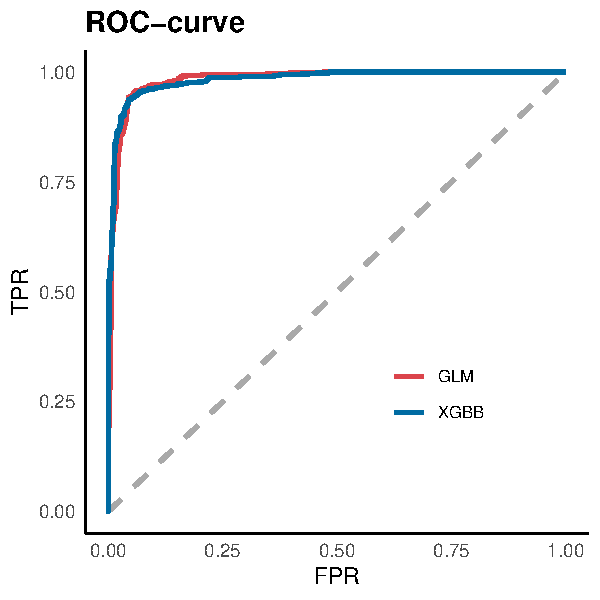
\includegraphics[width=0.5\linewidth]{images/roc_curve.pdf}
    \caption{{ROC Curve for 30-day predictions}}
    \subcaption*{Receiver operating characteristic (ROC) curve illustrated for the GLM30 and XGBB30 ML models. Area Under ROC is 0.9797 and 0.9812 for the GLM30 and XGBB30 respectively. }
    \label{fig:roc-curve-for-models}
\end{figure}

 \autoref{fig:roc-curve-for-models} show the ROC curve for models GLM and XGBB, for the 30-day prediction horizon. Compared to \autoref{fig:area-under-roc-curve-illustration}, the characteristics from the ROC-curve in \autoref{fig:roc-curve-for-models} seem to further support the models' overall ability to predict index-composition, supporting the findings from \autoref{table:accuracy-precision-sensitivity-specificity-f-score}. Notice that we did not include the XGBC models in this plot, because the plot is generated by using the estimated likelihoods from the models, which is the same for both XGBB and XGBC models.
 
\subsubsection{Accuracy over Time}

Furthermore, we illustrate the models' performance over time, as we are dealing with a time series. \autoref{fig:machine-learning-results} show the ML model's accuracy over time, completed with the number of changes (additions and deletions) predicted for each period, and the number of true changes captured. As expected from \autoref{table:accuracy-precision-sensitivity-specificity-f-score}, GLM and XGBB models seem to yield better accuracy for most periods, while predicting fewer changes than XGBC. Once again our results suggest a negative relationship between accuracy and the number of predicted changes. 

\begin{figure}[H]
    \centering
    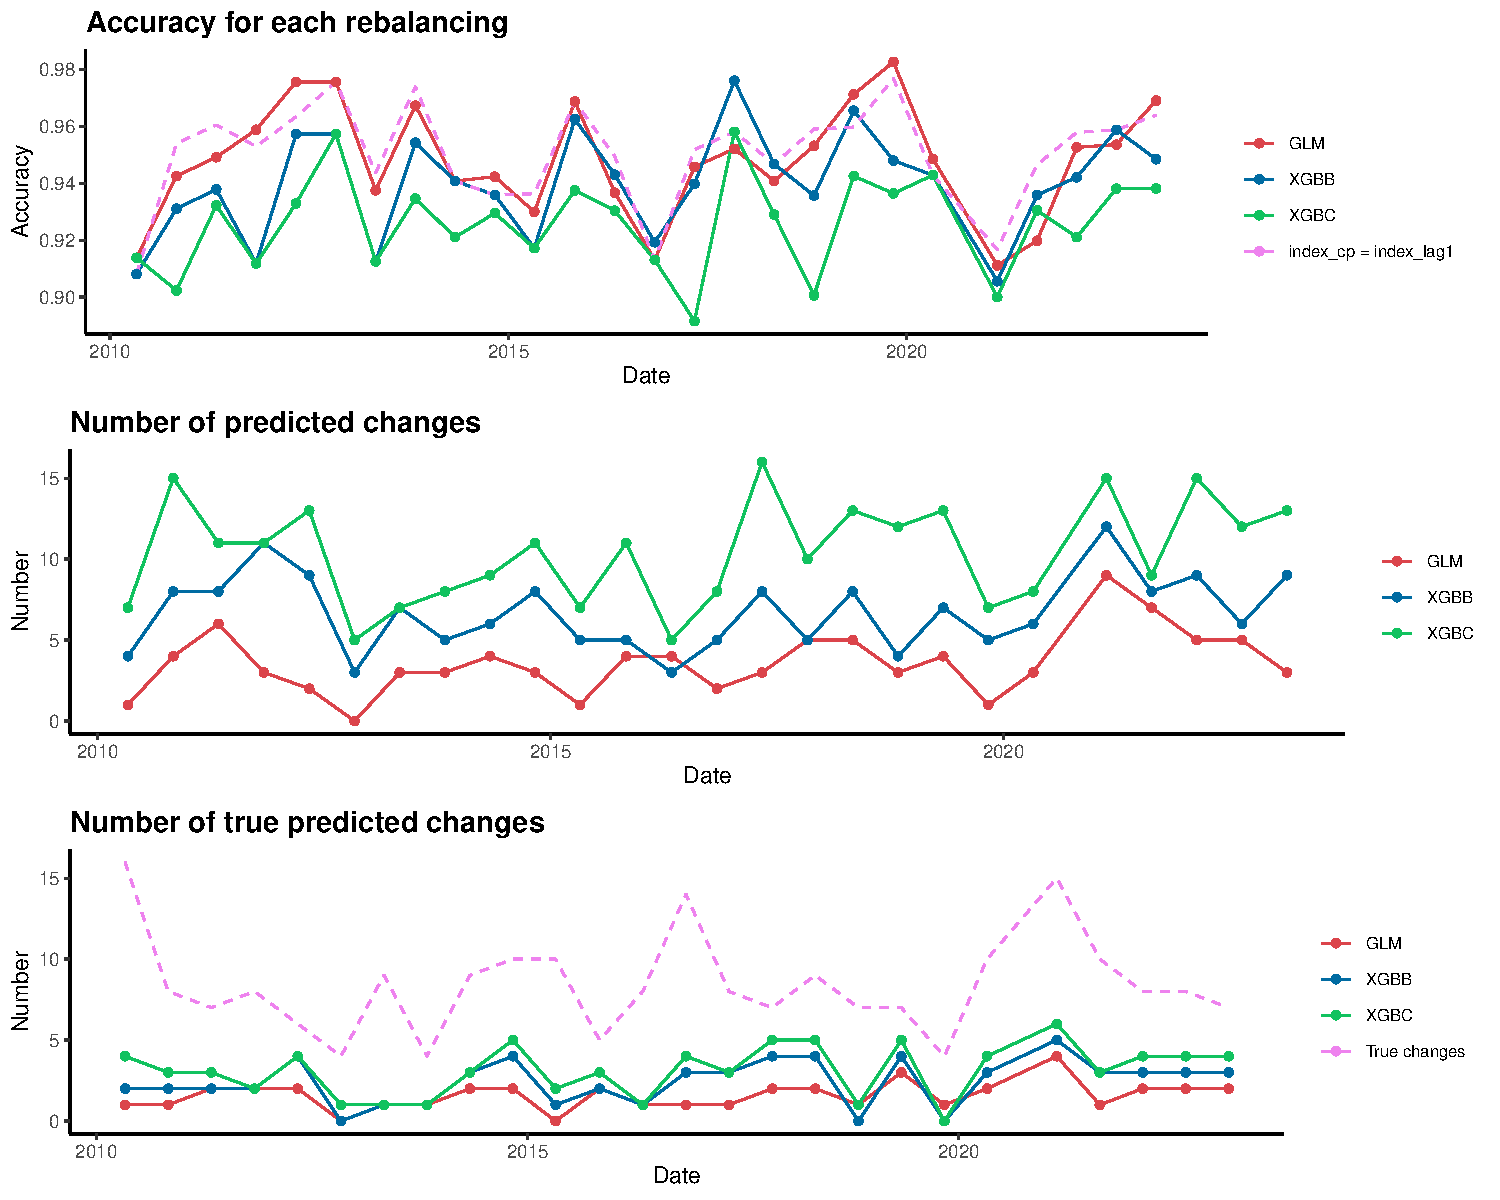
\includegraphics[width=\textwidth]{images/machinelearning_res.pdf}
    \caption{{ML Results over time, 30-day prediction horizon}}
    \subcaption*{Illustrations of how the models GLM30, XGBB30, and XGBC30 perform over the course of the period from 2010 to 2023. Please note that the simple model (index\_lag1) is illustrated in the accuracy plot. }
    \label{fig:machine-learning-results}
\end{figure}

Another insight from \autoref{fig:machine-learning-results} is that we are nowhere near capturing all true changes. As mentioned earlier, if we had bought all companies outside of OSEBX and sold all companies at OSEBX, we would have captured all the changes. However, that would significantly dilute the index effect, and we therefore need to keep accuracy at a reasonable level even for the XGBC models. From these results, we do however learn that the XGBC models are able to capture more of the true changes than the GLM and XGBB models.

\subsubsection{Variable Importance Plot}
We do already understand that the \texttt{index\_lag1} variable is important when predicting index composition, but we have yet to explore the importance of the remainder of the variables. \autoref{fig:variable-importance-plot-result} show variable importance for our GLM- and XGBoost models predicting 30 days prior to ED respectively.

\begin{figure}[H]
    \centering
    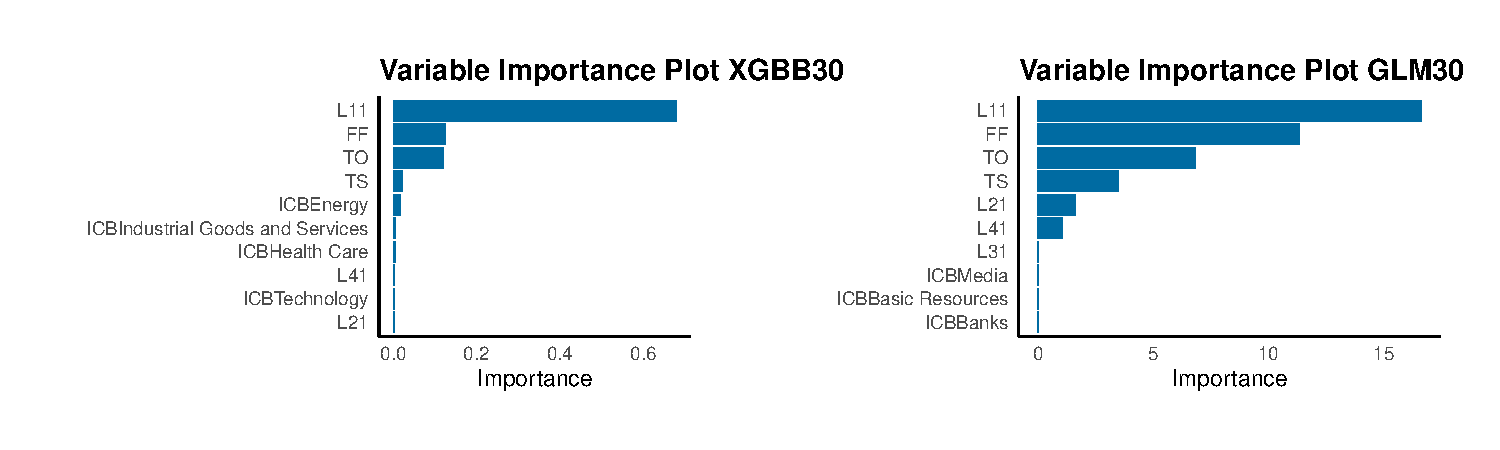
\includegraphics[width=\textwidth]{images/vip.pdf}
    \caption{{VIP for XGBB30 and GLM30}}
    \subcaption*{Please see \autoref{tab:final-data-set-predictor-target} for explanation for all variable abbreviations. Notice that the x-axis measurement differs between the two plots and each plot must be read independently.}
    \label{fig:variable-importance-plot-result}
\end{figure}

 For GLM and XGBB, the variable \texttt{index\_lag1} proves to be the most important one, followed by \texttt{free\_float}, \texttt{turnover\_eob}, and \texttt{trading\_status}. Understanding why \texttt{index\_lag1} is most important, we remember that most of the 50-80 companies on OSEBX stay from one period to the next. This includes large Norwegian companies, such as Equinor and Telenor. Therefore, predicting large and liquid companies staying on OSEBX from one period to the next is quite easy, with similar intuition for small listed companies staying off OSEBX. The \texttt{index\_lag1} variable is however not suited for explaining the cases where the model predicts a change in the response variable compared to the previous period. This must then be explained by the other variables, seemingly by \texttt{free\_float}, \texttt{turnover\_eob}, and \texttt{trading\_status}, which are the variables taken directly out of the OSEBX rule book. Furthermore, the two models differentiate when it comes to the 5th, 6th, and 7th most important variables. The GLM model seems to depend more on the other lag variables, whereas the XGBoost models are more dependent on the \texttt{icb\_supersector} variables. 


\subsubsection{Conclusion for Research Question (1)}

In our first research question, we ask "To what degree can ML predict index composition in the next period?". In this section, we have discussed the models' overall performance. The simple model which only predicts using \texttt{index\_lag1}, gave the highest accuracy (0.9507), but GLM100 followed closely with an accuracy of 0.9506. This means that we were able to predict more than 95\% of all observations correctly, and we conclude that ML algorithms can predict the upcoming index composition on OSEBX with high accuracy. Furthermore, we have in this section learned that there might exist a trade-off between model accuracy and the total number of predicted changes made by the ML algorithms. This finding is a \textit{central} insight in our thesis. This can cause great consequences in the following section where we simulate portfolios based on the predicted additions and deletions obtained by the models. 

% RESEARCH QUESTION 2 %%%%%%%%%%%%%%%%%%%%%%%%%%%%%%%%%%%%%%%%%%%%%%%%%%%

\subsection{Research Question (2): To what degree can trading on predicted additions and deletions outperform OSEBX in an active trading portfolio?}

In the previous section, we investigated the model accuracy of GLM and XGBoost. In this section, we simulate a portfolio in the period from 2010 to 2023, where we trade on the predicted additions and deletions made by our models. In the portfolio simulation, we consider the number of rebalancing events to predict. We have considered the data available, and find it is suitable for the first rebalancing period to start in 2010. In other words, the first train data set is from 2006 until the first test period in May of 2010. The portfolio simulation ended after the last rebalancing event of March 2023. 

\subsubsection{Active Trading Strategy}

Our trading strategy can be summarised as the following: we buy the companies that the ML models predict to enter OSEBX, and we sell the companies that the ML models predict to exit. The additions/deletions are bought/sold on the date of prediction, and sold/bought at ED. This has several implications. First, we are only allowed to buy companies that are not included in the index at the time of prediction, and we are only allowed to sell companies that currently are on the index. Second, it requires us to expand the strategy to manage the portfolios outside of the active trading period (outside the trading window between prediction and ED). As we want to beat OSEBX, we have decided to take a long position in OSEBX when outside of the trading window. This means that any potential excess returns must come from the active trading period. Thirdly, an important implication is that by using this strategy, we will \textit{never} trade against the index effect in the active period. This is because we are not allowed to buy companies exiting, and not allowed to sell companies entering. 


In a long position, one expects the stock price to rise, and in a short position, one expects the stock price to fall \parencite{jacobs-long-short}. Looking at the index effect in \autoref{fig:index-effect-osebx}, we would like to capture both the rising stock prices by going long on additions and falling stock prices by going short on deletions. In practice, this includes finding combinations where \texttt{index\_lag1=0} is paired with the predicted \texttt{index\_cp=1} (addition, we take a long position), or where \texttt{index\_lag1=1} is paired with the predicted \texttt{index\_cp=0} (deletion, we take a short position). In practice, we simulate two implementations of our strategy. The first strategy includes going long-short, meaning that we are allowed to go both long and short. On the contrary, our second strategy uses long-only positions. The portfolios we simulate and analyse can be summaries as in \autoref{tab:portfolio-names}. 

\begin{table}[H]
\centering
\footnotesize
\begin{tabularx}{\textwidth}{llXXX}
\hline
Model          & Strategy         & ED-30     & ED-60     & ED-100 \\
\hline
GLM           &   Long-short     & GLM30     & GLM60     & GLM100 \\
XGBoost Benchmark&  Long-short      & XGBB30    & XGBB60    & XGBB100 \\
XGBoost Custom  &  Long-short       & XGBC30    & XGBC60    & XGBC100 \\
\midrule
GLM            &   Long-only       & GLM30L     & GLM60L     & GLM100L \\
XGBoost Benchmark &  Long-only     & XGBB30L    & XGBB60L    & XGBB100L \\
XGBoost Custom    &   Long-only    & XGBC30L    & XGBC60L    & XGBC100L \\
\hline
\end{tabularx}
\vspace{1em}
\caption{{Simulated Portfolio Names}}
\subcaption*{Overview of the portfolio names. Notice that the portfolios trade on predicted changes made by the corresponding model from \autoref{tab:machine-learning-model-names}.  The long-short portfolios trade using both predicted additions and deletions. The long-only portfolios trade using only the predicted additions. Long-only portfolios are denoted by the suffix L at the end of the name. }
\label{tab:portfolio-names}
\end{table}

As mentioned in \autoref{introduction}, Euronext rebalances OSEBX twice each year, which is done on ED. Since 2020, ED has been the third Friday of March and September, and before 2020, ED was the first trading day of June and December. Depending on the prediction horizon of 30, 60, or 100 days prior to ED, the active portfolio will be significantly shorter than a year. \autoref{fig:timeline-investment-horizon} illustrates the timeline of the active trading portfolio investment horizon. 

\begin{figure}[H]
    \centering
    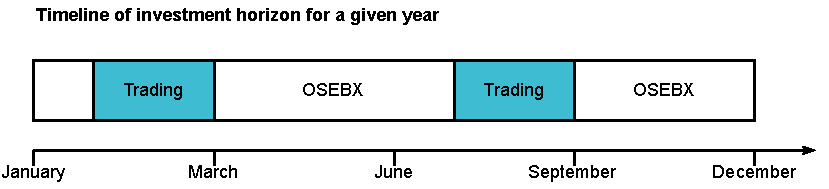
\includegraphics[width=\linewidth]{images/investment-horizon.drawio.pdf}
    \vspace{1em}
    \caption{{Timeline of Investment Horizon}}
    \subcaption*{During the year, our portfolios can be in two states. (1) in an active trading period, between the prediction and the ED. (2) in a passive period, meaning that the money is invested in OSEBX.}
    \label{fig:timeline-investment-horizon}
\end{figure}

\subsubsection{Financial Assumptions}
Next, we discuss the underlying financial assumptions of our portfolio simulation. These are important to make the results robust and practically applicable. The assumptions can be summarised as (1) transaction costs, (2) liquidity, (3) portfolio weights, and (4) interest rate on short positions.

Transaction costs include the brokerage fees when completing a trade \parencite{coase-transaction-costs}. This can come from either brokers implementing the trade by finding a counterpart directly or using a highly advanced trading algorithm supplied by a broker. Electronic trading algorithms typically have lower transaction costs and can utilise strategies, such as completing trades using VWAP. In the portfolio simulation, we take into account the transaction cost by subtracting a cost per trade made. We use basis points (bps) when discussing trading cost, where 1 bps is equal to 0.01\%. \textcite{nbim-investing-in-equities} report commission rates between 5$-$10 bps during the last two decades, with about 2 bps for electronic trades. \textcite{dnb-transaction-costs} list a fee of 4 bps per transaction for large private investors. In the portfolio simulation, we do electronic trades using VWAP, and assuming we can trade on the terms for large investors according to \textcite{dnb-transaction-costs}, we assume a transaction cost of 4 bps. 

Liquidity refers to the availability to which stocks can be traded without significantly altering their prices \parencite{hicks-liquidity}. In practice, stocks on OSEBX may not be available to trade at every given point in time. Still, we conclude that assuming full liquidity for our stocks can be justified. We will be trading stocks on OSEBX that either are on the index or are likely to be on it for the next period. Stocks of these types will have the characteristics of high \texttt{trading\_status}, representing high liquidity. Using this assumption, we say that all stocks are available, and trades are done using VWAP. 

For predicted trades made by the ML model, we must determine the weighting of each security in our active trading portfolio \parencite{frost-portfolio-weights}. We considered different approaches, either to (1) give stocks weights based on the estimated likelihood from the ML model, or to (2) give stocks equal weights. In a practical setting one could argue that weighting smaller or larger positions based on the statistical likelihood is an effective approach, although we decide to weight the positions equally. In short, this is due to ease of implementation, and a lack of an effective converter from probability to weight. 

When taking short positions, one has to borrow a number of stocks from a third party \parencite{jacobs-long-short}. This comes with an interest rate cost, as the original stock owner is compensated for giving up the opportunity to trade during the lending period. The short-position interest rate depends on a variety of factors, including supply of short-sellers. \textcite{nordnet-short-interest-rate} state a short-position interest rate of 4\% annually, and this is what we use in our simulations. Furthermore, regarding short positions, we have used a maximum limit of what the short position might rise to before we are forced to buy back the position. This limit is 100 \%, meaning that if the stock price doubles in value, then we are forced to buy it back and we will get a return of -100\%. In other words, this diminishes the loss, to the maximum loss in a long position.

To sum up, our financial assumptions aim to be conservative, but yet insight-full as shown in \autoref{tab:trading-financial-assumptions}. This is to increase the robustness of our findings and make them valid in a practical setting. 

\begin{table}[H]
\centering
\begin{tabular}{ll}
\hline
Financial & Assumption \\
\hline
Transaction cost trades   & 4 bps   \\ 
Transaction cost OSEBX  & 4 bps \\
Liquidity   & Full \\ 
Price  & VWAP \\ 
Stock weights in portfolio  & Equal \\ 
Risk-free rate $R_f$ & $\approx$ 1.46\% annually \\
Short-position interest rate & 4\% annually \\
\hline
\end{tabular}
\vspace{1em}
\caption{{Summary of Financial Assumptions in the Trading Portfolios}}
\subcaption*{These assumptions lay the basis for our simulations. They aim to be as accurate in a practical sense as possible. }
\label{tab:trading-financial-assumptions}
\end{table}

\subsubsection{Application of the Portfolio Simulations}

 Before presenting portfolio performance, we present a brief explanation to how the simulations are executed. First, the ML models generate a set of predictions, for 30-, 60-, and 100-days in advance of the ED. The data frame in which the predictions are stored is then filtered, so that only the cases where the prediction is different from the classification in the previous period are left. Next, the VWAP is extracted for each recommended trade on both ED and on the date of prediction, depending on the prediction horizon. The return of the position is then determined as shown in \autoref{return_explaination}, where $r_l$ is return on long-positions, and $r_s$ is return on short-positions, $p_0$ is the VWAP of the stock at the start of the trading period, and $p_1$ is the VWAP at the end. 

\begin{equation}
\begin{aligned}
    r_l = \frac{p_1 - p_0 }{p_0} &  ,  &r_s = \frac{p_0 - p_1 }{p_0} 
    
\label{return_explaination}
\end{aligned}
\end{equation}
Next, we take the average of each return per trading period (because we assume equal weighting in our portfolios), and use this return as the period return. This operation is done for each trading period, and we are left with the portfolio development over time. The amount of money that is held at the beginning of the trading period is then multiplied by the average growth factor (the average return plus 1). The same logic applies to the passive periods, where the money is invested in OSEBX. Transaction costs are applied at the start and end of each trading period, and the short interest rate is subtracted from the calculated return on any short position. This is explained in greater detail in \autoref{APPENDIX Portfolio Simulation Algorithm}. In \autoref{APPENDIX Portfolio Simulation of GLM100-portfolio} we also show an example of a simulated portfolio, namely the GLM100 portfolio.

\subsubsection{Performance in a Capital Asset Pricing Model}

 The financial metrics for our respective active trading portfolios are shown in \autoref{tab:new-performance-trading-return-sigma-sharpe-alpha-beta-te-ir}, sorted by decreasing SR. The results in \autoref{tab:new-performance-trading-return-sigma-sharpe-alpha-beta-te-ir} can be compared to the desired metrics in \autoref{tab:metrics-ranges-implications}. All calculations are done using monthly returns, except TE$_{ann}$. Notice that the names of portfolios in \autoref{tab:new-performance-trading-return-sigma-sharpe-alpha-beta-te-ir} correspond to the ML model used to generate trade predictions, as shown in \autoref{tab:portfolio-names}. 

\begin{table}[H]
\centering
\footnotesize
\begin{tabularx}{\textwidth}{Xllllllll}
\toprule
Portfolio & $R_p-R_b$ & $R_p$ & $\sigma_p$ & SR & $\alpha$_{CAPM} & $\beta$ & TE_{ann} & IR \\
\midrule
OSEBX & 0 & 0.0095 & 0.0423 & 0.1981 & 0.0002 & 1.0148 & 0.0000 &  \\ 
\midrule
   GLM60 & 0.0095  & 0.0190 & 0.0756 & 0.2367 & 0.0139 & 0.4966 & 0.2599 & 0.1268 \\ 
   GLM30 & 0.0034  & 0.0129 & 0.0511 & 0.2309 & 0.0048 & 0.8634 & 0.1260 & 0.0940 \\ 
  XGBC30 & 0.0017  & 0.0112 & 0.0441 & 0.2289 & 0.0026 & 0.9249 & 0.0789 & 0.0755 \\ 
  GLM100 & 0.0087  & 0.0182 & 0.0757 & 0.2257 & 0.0133 & 0.4684 & 0.2668 & 0.1132 \\ 
  XGBB30 & 0.0010  & 0.0105 & 0.0488 & 0.1917 & 0.0016 & 0.9536 & 0.1056 & 0.0321 \\  
  XGBC60 & -0.0029 & 0.0066 & 0.0480 & 0.1138 & -0.0004 & 0.7285 & 0.1383 & -0.0731 \\ 
  XGBB60 & -0.0019 & 0.0076 & 0.0608 & 0.1073 & 0.0020 & 0.5532 & 0.2095 & -0.0306 \\ 
 XGBC100 & -0.0038 & 0.0057 & 0.0443 & 0.1027 & 0.0017 & 0.3470 & 0.1782 & -0.0744 \\ 
 XGBB100 & -0.0058 & 0.0037 & 0.0539 & 0.0487 & -0.0012 & 0.4696 & 0.1947 & -0.1024 \\ 
 \midrule
 XGBC30L & 0.0032  & 0.0127 & 0.0482 & 0.2398 & 0.0034 & 1.0065 & 0.0903 & 0.1222 \\ 
 XGBB30L & 0.0033  & 0.0128 & 0.0500 & 0.2335 & 0.0033 & 1.0386 & 0.0990 & 0.1158 \\ 
  GLM30L & 0.0009  & 0.0104 & 0.0460 & 0.2011 & 0.0012 & 0.9942 & 0.0674 & 0.0450 \\ 
 XGBB60L & 0.0011  & 0.0106 & 0.0543 & 0.1751 & 0.0019 & 0.9428 & 0.1361 & 0.0288 \\ 
 XGBC60L & 0.0004  & 0.0099 & 0.0505 & 0.1737 & 0.0008 & 0.9843 & 0.1063 & 0.0131 \\ 
  GLM60L & 0.0002  & 0.0097 & 0.0553 & 0.1550 & 0.0002 & 1.0340 & 0.1187 & 0.0056 \\ 
XGBC100L & 0.0011  & 0.0106 & 0.0649 & 0.1468 & 0.0035 & 0.7391 & 0.2078 & 0.0191 \\
XGBB100L & 0.0015  & 0.0110 & 0.0682 & 0.146 & 0.00324 & 0.826 & 0.211 & 0.0255 \\ 
 GLM100L & -0.0031 & 0.0064 & 0.0669 & 0.0797 & -0.0033 & 1.0614 & 0.1809 & -0.0583 \\ 
\bottomrule
\end{tabularx}
\vspace{1em}
\caption{{CAPM Portfolio Performance for Active Trading Strategies Using Monthly Returns}}
\subcaption*{Risk free interest rate is $\approx$ 0.12 \% per month. The market return is assumed to be the return of OSEAX during the same period, which gave a monthly average return of $\approx$ 0.92\%. Both the risk-free interest rate and the market return are calculated based on (\cite{bernt-fama-french}) in the period from January 31st, 2010 to May 31st, 2022. TE and information ratio is calculated in relation to OSEBX, as this is the index we are aiming to beat. The table is sorted after SR. The analysed period is from January 31st, 2010 to May 31st, 2022. $R_b$ represents the return of the benchmark index OSEBX, so the first column shows excess returns in relation to OSEBX. }
\label{tab:new-performance-trading-return-sigma-sharpe-alpha-beta-te-ir}
\end{table}

Please note that we have defined the market to be OSEAX, as this is the pool of stocks we can buy or sell. Our first observation is that several portfolios yield higher returns $R_p$ than OSEBX. Especially the GLM portfolios yield exceptional returns (GLM60 yielding twice the return of OSEBX). However, those portfolios tend to also be involved with higher risk $\sigma_p$. Taking this into consideration, we observe SR, where the XGBC30L portfolio excels. It is, however, closely followed by the portfolios GLM60, GLM30, XGBC30, GLM100 and XGBB30L. All of these portfolios outperform OSEBX in terms of SR, which seems promising. Furthermore, we observe the biggest alphas $\alpha_{CAPM}$ in GLM60 and GLM100. The high $\alpha_{CAPM}$ for those two portfolios is likely caused by the low correlation with the market ($\beta$) and exceptional returns. At this stage, we would expect this $\alpha_{CAPM}$ to diminish after adjusting for FF3 later on. We also observe notable $\alpha_{CAPM}$ for GLM30, XGBC30, XGBC30L and XGBB30L. Furthermore, the calculated betas $\beta$ seems somewhat surprising, considering the risk $\sigma_p$ involved with several of the portfolios. In general, a risky portfolio is considered to have a high beta (namely, greater than 1). In the long-short portfolios we do however trade on short-positions, which in the active trading periods can constitute a negative correlation with the market, and in turn, lower the beta $\beta$ (being the correlation coefficient with the market). When considering the long-only portfolios we observe somewhat more expected results, with $\beta$ varying from 0.73 to 1.04. In conclusion, several models outperform OSEBX in the world of CAPM, both on $R_p$, $SR$, and $\alpha_{CAPM}$. Further, we investigate the portfolio's exposure to risk.

\subsubsection{Fama-French 3 factor Model on Active Portfolios}

Going further than CAPM portfolio performance, we want to understand if the excess returns can be explained by the risk factors in an FF3 model. We run a linear regression using portfolio returns minus risk-free rate as the dependent variable, and factors SMB, HML, and the market risk premium (see \autoref{Theoretical background}) as independent variables. The FF3 factors introduced in \autoref{Theoretical background} are retrieved from \textcite{bernt-fama-french}, as discussed in \autoref{Data}. 

Note that \textcite{bernt-fama-french} report Fama-French factors for OSE, which is somewhat different from OSEBX. Because OSEAX represents more of the companies on OSE than OSEBX does, we argue that the risk factors are representing OSEAX to a higher extent than OSEBX. We therefore use OSEAX as the market in the FF3 regressions. We have also done the same regressions using OSEBX as the market, which is shown in \autoref{ff3-osebx}, to check for any significant differences.


% new updated 14.12.2023
\begin{table}[H] 
\centering 
\footnotesize
\begin{tabularx}{\textwidth}{XXXX|XXX|XXX|l} 
\\[-2ex]\hline 
\hline \\[-2ex] 
 & \multicolumn{10}{c}{\textit{Dependent variable:}} \\ 
\cline{2-11} 
\\[-2ex] 
 & \multicolumn{3}{c}{GLM} & \multicolumn{3}{c}{XGBB} & \multicolumn{3}{c}{XGBC} & \\
 \cline{2-10}
 \\[-2ex] 
 & 30 & 60 & 100 & 30 & 60 & 100 & 30 & 60 & 100 & OSEBX \\ 
 \cline{2-10} \\
 MR & 0.890$^{***}$ & 0.553$^{***}$ & 0.510$^{***}$ & 0.958$^{***}$ & 0.545$^{***}$ & 0.457$^{***}$ & 0.938$^{***}$ & 0.729$^{***}$ & 0.337$^{***}$ & 1.022$^{***}$ \\ 
  & (0.075) & (0.149) & (0.151) & (0.060) & (0.117) & (0.104) & (0.046) & (0.078) & (0.087) & (0.017) \\
   & & & & & & & & & & \\ 
 SMB & $-$0.166$^{**}$ & $-$0.133 & $-$0.129 & $-$0.105$^{*}$ & $-$0.068 & 0.138 & $-$0.124$^{***}$ & $-$0.058 & 0.101 & $-$0.042$^{**}$ \\ 
  & (0.076) & (0.150) & (0.152) & (0.061) & (0.117) & (0.104) & (0.046) & (0.078) & (0.087) & (0.017) \\ 
   & & & & & & & & & & \\ 
 HML & $-$0.055 & $-$0.219$^{**}$ & $-$0.153 & 0.029 & 0.070 & $-$0.005 & $-$0.008 & 0.023 & 0.007 & $-$0.016 \\ 
  & (0.056) & (0.110) & (0.112) & (0.045) & (0.086) & (0.077) & (0.034) & (0.058) & (0.064) & (0.013) \\ 
   & & & & & & & & & & \\ 
 $\alpha$_{FF3} & 0.006$^{**}$ & 0.013$^{**}$ & 0.013$^{**}$ & 0.003 & 0.004 & $-$0.003 & 0.004$^{**}$ & 0.001 & 0.0004 & 0.001 \\ 
  & (0.003) & (0.006) & (0.007) & (0.003) & (0.005) & (0.004) & (0.002) & (0.003) & (0.004) & (0.001) \\ 
   & & & & & & & & & & \\   
\hline \\[-3ex] 
Obs & 148 & 148 & 148 & 148 & 148 & 148 & 148 & 148 & 148 & 148 \\ 
R$^{2}$ & 0.494 & 0.099 & 0.078 & 0.647 & 0.145 & 0.138 & 0.746 & 0.388 & 0.112 & 0.962 \\ 
R$^{2}$_{adj} & 0.484 & 0.080 & 0.059 & 0.639 & 0.127 & 0.120 & 0.740 & 0.375 & 0.093 & 0.961 \\ 
\hline 
\hline \\[-2ex] 
\textit{Note:}  & \multicolumn{10}{r}{$^{*}$p$<$0.1; $^{**}$p$<$0.05; $^{***}$p$<$0.01} \\ 
\end{tabularx}
\vspace{1em}
\caption{{FF3 Regression: Long-Short Active Portfolios}} 
\subcaption*{The table shows the regression summary of the long-short portfolios return net of risk-free interest rate against market risk premium (RM), the small minus big factor (SMB), and the high minus low factor (HML). The market is considered to be OSEAX, the same as we used as the market used in \autoref{tab:new-performance-trading-return-sigma-sharpe-alpha-beta-te-ir}. Notice that the factors are reported for OSE, and was obtained by \textcite{bernt-fama-french}. We, therefore, decided to use OSEAX as the market, as this more closely represents the market that the factors express.
}
\label{fama-french-trading-long-short} 
\end{table} 


In \autoref{fama-french-trading-long-short}, we find statistically significant positive alpha $\alpha_{FF3}$ at a 95\% confidence level for portfolios GLM30, GLM60, GLM100, and XGBC30, all outperforming the benchmark index OSEBX $\alpha_{FF3}$ of 0.001. This indicates that the mentioned portfolios produce excess returns that are not fully explained by FF3. In comparison to the findings in \autoref{tab:new-performance-trading-return-sigma-sharpe-alpha-beta-te-ir}, we see that the GLM60 and GLM100 portfolios diminish in FF3-regression (compared to the $\alpha_{CAPM}$ reported in CAPM), whereas both GLM30 and XGBC30 increases slightly. This can suggest that the GLM30 and XGBC30 have negative exposure to the risk factors. This is further supported by the correlation coefficients for both SMB and HML. There might also be a source of error coming from the difference between what we have defined as the market, OSEAX, and OSE, on which the risk factors are based. 

% 14 december fama french
\begin{table}[H] \centering  
\footnotesize
\begin{tabularx}{\textwidth}{XXXX|XXX|XXX|l} 
\\[-2ex]\hline 
\hline \\[-2ex] 
 & \multicolumn{10}{c}{\textit{Dependent variable:}} \\ 
\cline{2-11} 
\\[-2ex] 
 & \multicolumn{3}{c}{GLML} & \multicolumn{3}{c}{XGBBL} & \multicolumn{3}{c}{XGBCL} & \\
 \cline{2-10}
 \\[-2ex] 
 & 30 & 60 & 100 & 30 & 60 & 100 & 30 & 60 & 100 & OSEBX \\ 
 \cline{2-10} \\
 MR & 1.001$^{***}$ & 1.042$^{***}$ & 1.066$^{***}$ & 1.030$^{***}$ & 0.936$^{***}$ & 0.795$^{***}$ & 1.006$^{***}$ & 0.984$^{***}$ & 0.719$^{***}$ & 1.022$^{***}$ \\ 
  & (0.045) & (0.074) & (0.104) & (0.055) & (0.079) & (0.025) & (0.052) & (0.064) & (0.118) & (0.017) \\ 
   & & & & & & & & & & \\ 
 SMB & $-$0.072 & 0.026 & 0.143 & 0.003 & 0.055 & 0.264 & $-$0.007 & 0.032 & 0.170 & $-$0.042$^{**}$ \\ 
  & (0.045) & (0.074) & (0.105) & (0.055) & (0.080) & (0.025) & (0.053) & (0.064) & (0.119) & (0.017) \\ 
   & & & & & & & & & & \\ 
 HML & 0.001 & $-$0.056 & $-$0.098 & 0.038 & 0.005 & 0.017 & 0.002 & $-$0.020 & 0.024 & $-$0.016 \\ 
  & (0.033) & (0.054) & (0.077) & (0.041) & (0.059) & (0.018) & (0.039) & (0.047) & (0.088) & (0.013) \\ 
   & & & & & & & & & & \\ 
 $\alpha$_{FF3} & 0.002 & $-$0.001 & $-$0.006 & 0.004 & 0.001 & $-$0.001 & 0.004 & 0.0002 & 0.001 & 0.001 \\ 
  & (0.002) & (0.003) & (0.005) & (0.002) & (0.003) & (0.001) & (0.002) & (0.003) & (0.005) & (0.001) \\ 
   & & & & & & & & & & \\ 
\hline \\[-2ex] 
Obs & 148 & 148 & 148 & 148 & 148 & 148 & 148 & 148 & 148 & 148 \\ 
R$^{2}$ & 0.783 & 0.588 & 0.437 & 0.720 & 0.505 & 0.189 & 0.727 & 0.634 & 0.229 & 0.962 \\ 
R$^{2}$_{adj} & 0.778 & 0.579 & 0.425 & 0.714 & 0.494 & 0.172 & 0.721 & 0.626 & 0.213 & 0.961 \\ 

\hline 
\hline \\[-2ex] 
\textit{Note:}  & \multicolumn{10}{r}{$^{*}$p$<$0.1; $^{**}$p$<$0.05; $^{***}$p$<$0.01} \\ 
\end{tabularx} 
\vspace{1em}
  \caption{{FF3 Regression: Long-Only Active Portfolios}} 
  \subcaption*{
  The table shows the regression summary of the long-only portfolios' return net of risk-free interest rate against market risk premium (RM), the small minus big factor (SMB), and the high minus low factor (HML). The market is considered to be OSEAX, similar to the market used in \autoref{tab:new-performance-trading-return-sigma-sharpe-alpha-beta-te-ir}. Notice that the factors are reported for OSE, and was obtained by \textcite{bernt-fama-french}}
  \label{fama-french-trading-long-only}
\end{table}

Looking at \autoref{fama-french-trading-long-only}, we do not get the same alphas as we did for the long-short portfolios. In the long-only portfolios, most portfolios are positively correlated with the risk factors (but not on a significant level). This might explain why we are unable to get significant alphas $\alpha_{FF3}$ in the long-only portfolios. We also see that most alphas decrease in contrast to the calculated alphas in \autoref{tab:new-performance-trading-return-sigma-sharpe-alpha-beta-te-ir}, indicating that the long-only portfolios are relatively exposed to the risk factors.

\subsubsection{Plot of Portfolios}

Next, we plot the portfolios with their cumulative return to get a more visual representation of their performance. The long-short active portfolios are shown in \autoref{fig:long-short-top-5}. This is the GLM30, GLM60, GLM100 and XGBC30. The corresponding long-only portfolios are plotted in the in \autoref{fig:long-only-top-5}. Notice that we have only plotted the portfolios yielding a significant alpha in FF3. All portfolios are plotted in \autoref{APPENDIX-Descriptive-statistics}, in \autoref{fig:long-short-all} and \autoref{fig:long-only-all}. In the same appendix, we also plotted so-called perfect portfolios, which are simulated knowing all additions and deletions, in \autoref{fig:trading-perfect}.

\begin{figure}[H]
    \centering
    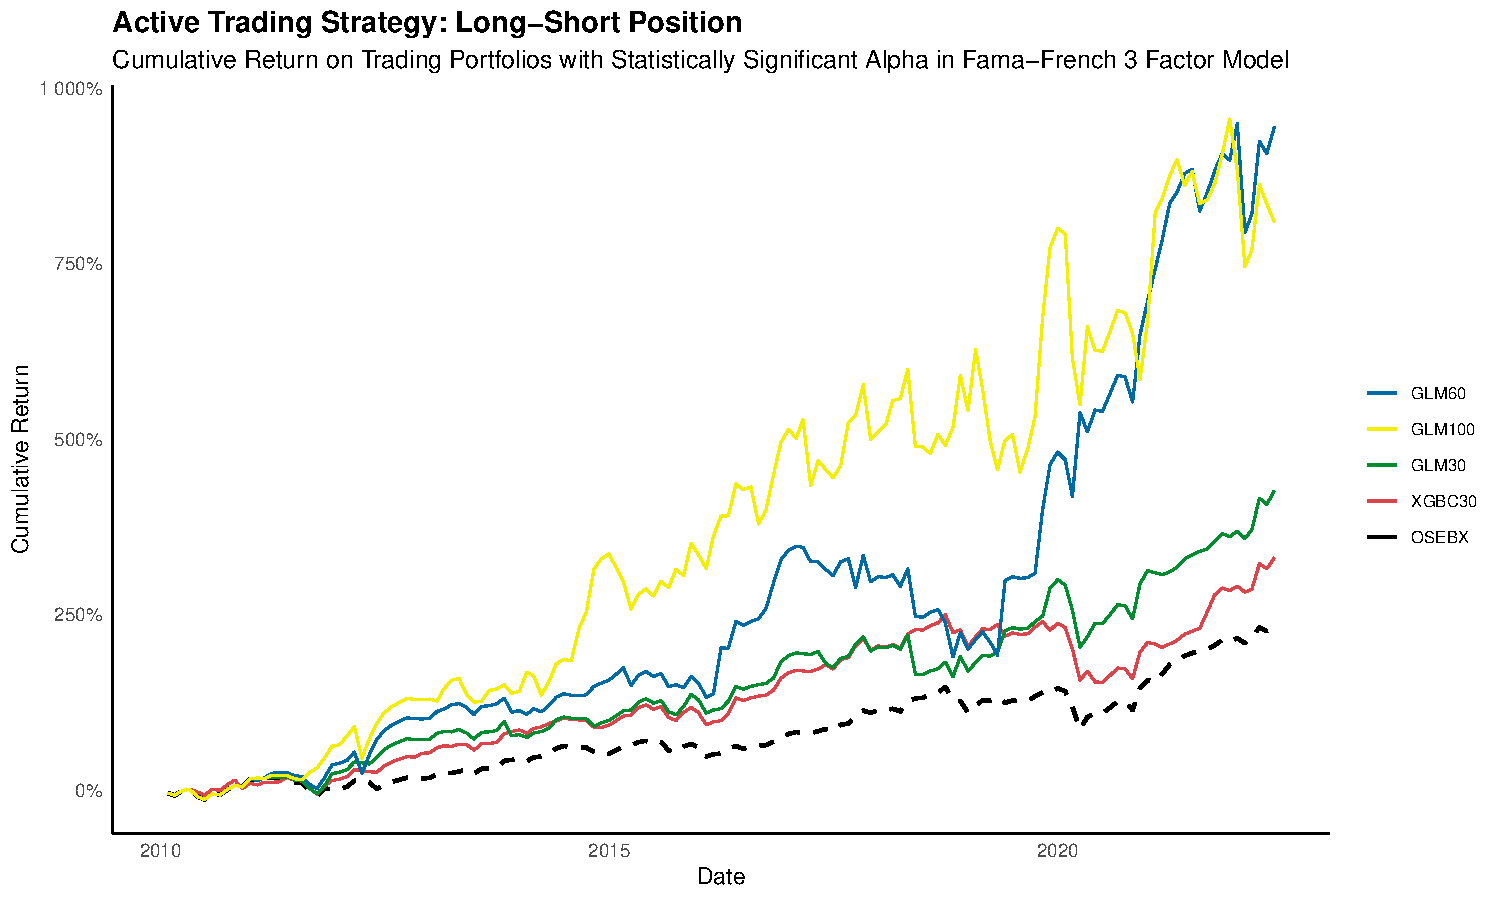
\includegraphics[width=0.85\textwidth]{images/trading_long_short.pdf}
    \caption{{Cumulative Return Long-Short Active Trading Strategy}}
    \subcaption*{Cumulative return for GLM30, GLM60, GLM100 and XGBC30, which all shows a significant alpha in the FF3-regression. OSEBX is also displayed. The GLM60 and GLM100 portfolios provide great investment opportunity for the risk-seeking investor.}
    \label{fig:long-short-top-5}
\end{figure}

\begin{figure}[H]
    \centering
    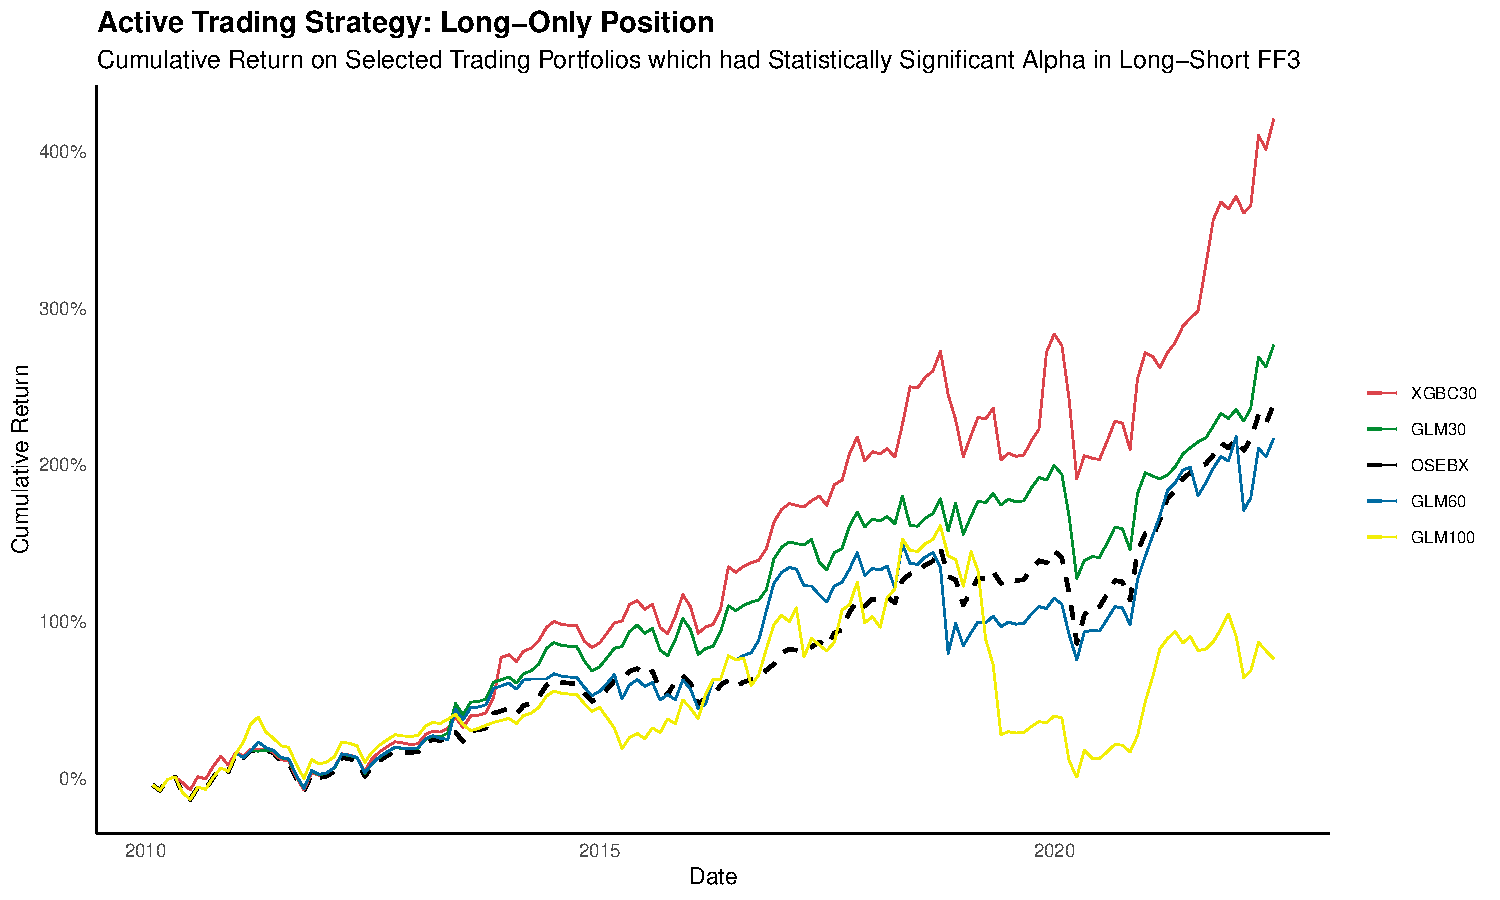
\includegraphics[width=0.85\textwidth]{images/trading_long_only.pdf}
    \caption{{Cumulative Return Long-Only Active Trading Strategy}}
    \subcaption*{Cumulative return for GLM30, GLM60, GLM100 and XGBC30, which all shows a significant alpha in the FF3-regression. OSEBX is also displayed. Still great returns for XGBC30 and GLM30, not so much for GLM60 and GLM100.}
    \label{fig:long-only-top-5}
\end{figure}

The cumulative return illustrated in \autoref{fig:long-short-top-5} shows that the GLM60 and GLM100 portfolios are yielding exceptional returns, though severely volatile. Those two portfolios are significantly affected by the low number of shares held in the active trading period, which varies between 1 and 6 companies. In contrast, the XGBC30 portfolio consist of about five times more, and still made for a significant alpha in the FF3-regression. Considering the long-only portfolios in \autoref{fig:long-only-top-5}, a different pattern emerges, where XGBC30L yields the highest returns, and the GLM60L and GLM100L perform worse than OSEBX when considering cumulative return. The predictions made by model XGBC30 seem to perform well in both strategies, and the increased number of shares seems to lower the risk in practice.

\subsubsection{Conclusion for Research Question (2)}
In this section, we have presented and discussed the results, to answer the research question: ”To what degree can trading on predicted additions and deletions outperform OSEBX in an active trading portfolio?". In this research question, we find that two types of very different portfolios tend to perform well. (1) The GLM portfolios predict few changes, but obtain excellent return on the few trades they do. (2) The XGBC30 portfolio can also obtain excellent returns but with a level of risk matching the benchmark, by predicting more changes than the GLM portfolios. Both directions tend to outperform OSEBX and have shown significant alphas in FF3. This is a \textit{key insight} in exploiting the index effect. Based on the results, it becomes evident that trading on predicted additions and deletions has proven to outperform OSEBX for the last 13 years, and we conclude that this strategy can outperform OSEBX to a high degree.  




% RESEARCH QUESTION 3 %%%%%%%%%%%%%%%%%%%%%%%%%%%%%%%%%%%%%%%%%%%%%%%%%%%

\subsection{Research Question (3): To what degree can trading on predicted additions and deletions outperform OSEBX in an enhanced index portfolio?}

In the previous two sections, we assessed the ML model performance of GLM and XGBoost and also applied them in an active trading strategy. Now we want to go further and investigate if such an active trading strategy can be combined with passive index investing to create an enhanced index portfolio, outperforming OSEBX.

\subsubsection{Enhanced Index Strategy}\label{Enhanced}

The enhanced index strategy seeks to combine the active trading strategy with an otherwise passive index portfolio. As discussed in \autoref{introduction}, defining enhanced index can be difficult \parencite{riepe-werner-are-enhanced-index-mutual-funds-worthy-of-their-name}. \textcite{ssg-tracking-error-enhanced} report that index investing can be considered "enhanced" with a TE in the continuum from 0.5\% to 2\%. We have decided to use a TE$_{ann}$ of 2\%, which is in the upper range of enhanced index. This enables us to more easily compare portfolio performances (as performance differences will grow with active share and TE). 

In practice, we adjust some of the financial assumptions, and run the simulations again, and use those to combine with OSEBX to construct enhanced index portfolios. We illustrate the enhanced index strategy in \autoref{fig:timeline-enhanced-index-investment-horizon}. Compared to the active trading strategy in \autoref{fig:timeline-investment-horizon}, we see that the active share is smaller, and the portfolio as a whole can therefore move closer to the benchmark index OSEBX. Note that we still use OSEBX as a benchmark index, which we calculate TE against, while we use OSEAX as the market in financial models.

\begin{figure}[H]
    \centering
    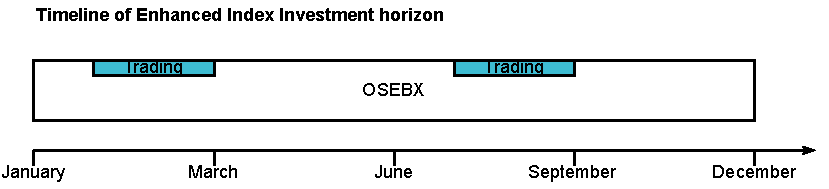
\includegraphics[width=\linewidth]{images/enhanced-index-investment-horizon.drawio.pdf}
    \vspace{1em}
    \caption{{Timeline of Enhanced Index Investment horizon}}
    \subcaption*{In the enhanced index portfolios, the active trading constitutes only for a smaller part of the total portfolio, which is dominated by OSEBX. }\vspace{1em}
    \label{fig:timeline-enhanced-index-investment-horizon}
\end{figure}

The simulated enhanced index funds consist of two parts. (1) The active share, which is a portfolio similar to those analysed in the previous section, and (2) The passive share, which is invested in OSEBX at all times. In contrast to the active trading perspective discussed in the previous section, we are now forced to own both the passive and the active share at the same time. The return of the enhanced index portfolios can be expressed as shown in \autoref{return_combined_port}, where $r_E$ is the return on the enhanced index portfolio, $r_A$ is the return on the active share, $r_P$ is the return of the passive share, and $s$ describes how big the active share is in the enhanced index portfolio. 

\begin{equation}
\begin{aligned}
    r_E =  r_A*s + r_P * (1-s)
\label{return_combined_port}
\end{aligned}
\end{equation}

\subsubsection{Financial Assumptions}

From the perspective of enhanced index portfolios, we face different challenges than those from the active trading portfolios. In this section, we are going to explore the most significant assumptions regarding the enhanced index portfolio, which can be broken down into interest rate on short positions, and share of active management.

We assume that by using an enhanced index strategy, we are managing a larger enhanced index fund, that follows OSEBX closely. By making this assumption, we always own stocks on OSEBX before each active investment horizon. This changes the assumption regarding short-position interest rates. Most importantly, we do not have to pay interest rates on the short positions. We would simply sell the positions because we already own them in the passive portfolio. Therefore, we simulate the active portfolios again, but this time without using interest rates on any short positions. 

Second, we assume that we are not allowed to operate outside the annual TE of 2\%. This limits how big a share of active management we can allow for throughout the year. How large the active management can be will depend on the prediction horizon of 30, 60, or 100 days, and also the volatility of the active portfolio. In this thesis, we have maximised the active share, given that TE cannot exceed 2\% annually. The weighting of the active share is therefore significantly varied between the portfolios. In general, the active portfolios with higher volatility are paired with a lower active share in the enhanced index portfolios. The weightings are shown in table \autoref{weights}. 

Third, the assumptions made in the previous section also apply in the context of an enhanced index portfolio, namely the assumptions regarding transaction costs, liquidity, and active portfolio weights (equal weighting of the companies held in the active part of the portfolio).

\subsubsection{Application of the Enhanced Portfolio Simulations}

The practical implementation of our enhanced index portfolio simulation closely mirrors that of the active trading portfolio simulation, but the main difference is that the enhanced portfolio is a combination of the active and the passive share. In practice, we first run new simulations of the active portfolios, without interest rates on short positions. Next, we optimise each active share, to yield a TE of 2\%. Finally, we analyse the performance of the enhanced index portfolios which are put together by combining the passive and active share using the weighting presented in \autoref{weights}.

\begin{table}[H]
\footnotesize
\center
\begin{tabular}{llll}
\toprule
Enhanced Portfolio & Active Share & Passive Share & TE_{ann} \\ 
\midrule
GLM30L & 0.267 & 0.733 & 2\% \\ 
XGBC30 & 0.221 & 0.779 & 2\%\\ 
XGBC30L & 0.182 & 0.818 & 2\%\\ 
GLM60L & 0.170 & 0.830 & 2\%\\ 
XGBB30 & 0.166 & 0.834 & 2\%\\ 
XGBB30L & 0.166 & 0.834 & 2\%\\ 
XGBC60L & 0.159 & 0.841 & 2\%\\ 
XGBC60 & 0.141 & 0.859 & 2\%\\ 
XGBB60L & 0.126 & 0.874 & 2\%\\ 
GLM100L & 0.124 & 0.876 & 2\%\\ 
GLM30 & 0.123 & 0.877 & 2\% \\ 
XGBC100 & 0.112 & 0.888 & 2\% \\ 
XGBB100 & 0.110 & 0.890 & 2\% \\ 
XGBC100L & 0.098 & 0.902 & 2\% \\ 
XGBB60 & 0.080 & 0.920 & 2\% \\ 
XGBB100L & 0.066 & 0.934 & 2\% \\ 
GLM60 & 0.041 & 0.959 & 2\% \\ 
GLM100 & 0.028 & 0.972 & 2\% \\ 
\bottomrule
\end{tabular}
\vspace{1em}
\caption{{Active and Passive Share in Enhanced Index Portfolios}}
\subcaption*{All portfolios are constructed to maximise the active share, and the constraint of TE cannot exceed 2\% per year. The active share represents the simulated portfolio trading on predicted additions/deletions, and the passive share is OSEBX.}
\label{weights}
\end{table}

In \autoref{weights}, we present the maximum weightings of the active share which is allowed in the enhanced index portfolios. This results in some interesting observations. First, we observe that the two most extreme active portfolios from the previous section (namely GLM60 and GLM100) are only allowed to constitute 4.1\% and 2.8\% as the active shares respectively. Secondly, the low-risk active portfolios like GLM30L (26.7\%), XGBC30 (22.1\%), and XGBC30L (18.2\%) are allowed to constitute an active share of several times more than the extreme portfolios.

\subsubsection{Performance in the Capital Asset Pricing Model}

Next, we investigate enhanced index portfolio performance. \autoref{tab:CAPM-PERFORMANCE-ENHANCED-INDEX} illustrate performance for the portfolios, sorted by decreasing SR. Notice that the name of the portfolio in \autoref{tab:CAPM-PERFORMANCE-ENHANCED-INDEX} corresponds to the active portfolio from \autoref{tab:machine-learning-model-names} used as the active share (without interest rate on short positions). 

% CAPM RESULTS
\begin{table}[H]
\centering
\footnotesize
\begin{tabularx}{\textwidth}{Xllllllll}
\toprule
Portfolio & $R_p-R_b$ & $R_p$ & $\sigma_p$    & SR & $\alpha$_{CAPM}  & $\beta$  & TE_{ann} & IR \\
\midrule
OSEBX &  0 & 0.0095 & 0.0423 & 0.1981 & 0.0002 & 1.0148 & 0.0000 &  \\ 
\midrule
GLM60 &  0.0005  & 0.0100 & 0.0410 & 0.2180 & 0.0011 & 0.9735 & 0.0200 & 0.0971 \\ 
GLM30 &  0.0005  & 0.0100 & 0.0418 & 0.2117 & 0.0008 & 0.9915 & 0.0200 & 0.0802 \\ 
GLM100 &  0.0003  & 0.0098 & 0.0412 & 0.2112 & 0.0008 & 0.9812 & 0.0200 & 0.0572 \\ 
XGBC30 &  0.0004  & 0.0099 & 0.0416 & 0.2111 & 0.0008 & 0.9933 & 0.0200 & 0.0721 \\ 
XGBB30 &  0.0001  & 0.0096 & 0.0420 & 0.2026 & 0.0004 & 1.0046 & 0.0200 & 0.0225 \\ 
XGBC100 &  -0.0005  & 0.0090 & 0.0392 & 0.2024 & 0.0003 & 0.9378 & 0.0200 & -0.0771 \\ 
XGBB60 &  -0.0003  & 0.0092 & 0.0407 & 0.2001 & 0.0003 & 0.9702 & 0.0200 & -0.0413 \\ 
XGBC60 &  -0.0004  & 0.0091 & 0.0407 & 0.1958 & 0.0001 & 0.9715 & 0.0200 & -0.0693 \\ 
XGBB100 &  -0.0006  & 0.0089 & 0.0399 & 0.1958 & 0.0001 & 0.9545 & 0.0200 & -0.0970 \\
\midrule
XGBC30L &  0.0006  & 0.0101 & 0.0423 & 0.2129 & 0.0008 & 1.0144 & 0.0200 & 0.1105 \\ 
XGBB30L &  0.0006  & 0.0101 & 0.0425 & 0.2112 & 0.0007 & 1.0217 & 0.0200 & 0.1033 \\ 
GLM30L &  0.0002  & 0.0097 & 0.0425 & 0.2021 & 0.0004 & 1.0083 & 0.0200 & 0.0359 \\ 
XGBC100L &  0.0000  & 0.0095 & 0.0414 & 0.2015 & 0.0003 & 0.9908 & 0.0200 & -0.0057 \\ 
XGBB60L &  0.0000  & 0.0095 & 0.0420 & 0.2008 & 0.0003 & 1.0044 & 0.0200 & 0.0104 \\ 
XGBB100L &  0.0000  & 0.0095 & 0.0420 & 0.1995 & 0.0002 & 1.0034 & 0.0200 & -0.0006 \\ 
XGBC60L &  0.0000  & 0.0095 & 0.0423 & 0.1982 & 0.0002 & 1.0092 & 0.0200 & 0.0004 \\ 
GLM60L &  -0.0001  & 0.0094 & 0.0429 & 0.1942 & 0.0001 & 1.0190 & 0.0200 & -0.0087 \\ 
GLM100L &  -0.0004  & 0.0091 & 0.0426 & 0.1872 & -0.0003 & 1.0180 & 0.0200 & -0.0705 \\ 
\bottomrule
\end{tabularx}
\vspace{1em}
\caption{{CAPM Portfolio Performance for Enhanced Index Strategies using Monthly Returns}}
\subcaption*{Risk free interest rate is $\approx$ 0.12 \% per month. The market return is assumed to be the return of OSEAX during the same period, which gave a monthly average return of $\approx$ 0.92\%. Both risk free interest rate and market return is calculated based on (\cite{bernt-fama-french}) in the period from January 31st 2010 to May 31st 2022. The TE and information ratio is calculated in relation to OSEBX, as this is the index we are aiming to beat. The table is sorted after SR. The analysed period is from January 31st 2010 to May 31st 2022. }
\label{tab:CAPM-PERFORMANCE-ENHANCED-INDEX}
\end{table}

Looking at \autoref{tab:CAPM-PERFORMANCE-ENHANCED-INDEX}, we find that GLM portfolios once again yield high SR, closely followed by XGBC30, XGBC30L, and XGBB30L. Also, when looking at the alpha $\alpha_{CAPM}$, GLM60 yields the highest, followed by GLM30, GLM100, XGBC30 and XGBC30L. In the enhanced portfolio simulation, the XGBC30L portfolio outperforms OSEBX the most, which seems to be a result of it being allowed to constitute for a significantly larger share (18.2\%) than the competing volatile portfolios. As we observed in the analysis of the active portfolios in the previous section, we see a tendency where the two styles of portfolios seem to outperform OSEBX. The first one is the high-yielding volatile portfolios, such as GLM60 and GLM100, and the second one is the diverse, low-risk portfolios.  

\subsubsection{Fama-French 3-factor Model}

In \autoref{fama-french-enhanced-long-short} and \autoref{fama-french-enhanced-long-only} we show FF3 regressions for long-short and long-only enhanced index portfolios respectively. 

% siste final allersiste oppdatert alt stemmer last and final update. Long short
\begin{table}[H] \centering 
\footnotesize
\begin{tabularx}{\textwidth}{XXXX|XXX|XXX|l} 
\\[-2ex]\hline 
\hline \\[-2ex] 
 & \multicolumn{10}{c}{\textit{Dependent variable:}} \\ 
\cline{2-11} 
\\[-2ex] 
 & \multicolumn{3}{c}{GLM} & \multicolumn{3}{c}{XGBB} & \multicolumn{3}{c}{XGBC} & \\
 \cline{2-10}
 \\[-2ex] 
 & 30 & 60 & 100 & 30 & 60 & 100 & 30 & 60 & 100 & OSEBX \\ 
 \cline{2-10} \\
 MR & 1.001$^{***}$ & 0.984$^{***}$ & 0.992$^{***}$ & 1.011$^{***}$ & 0.976$^{***}$ & 0.959$^{***}$ & 1.002$^{***}$ & 0.977$^{***}$ & 0.943$^{***}$ & 1.022$^{***}$ \\ 
  & (0.021) & (0.020) & (0.020) & (0.018) & (0.019) & (0.018) & (0.019) & (0.019) & (0.017) & (0.017) \\ 
   & & & & & & & & & & \\ 
 SMB & $-$0.060$^{***}$ & $-$0.046$^{**}$ & $-$0.047$^{**}$ & $-$0.054$^{***}$ & $-$0.047$^{**}$ & $-$0.027 & $-$0.064$^{***}$ & $-$0.046$^{**}$ & $-$0.027 & $-$0.042$^{**}$ \\ 
  & (0.021) & (0.020) & (0.020) & (0.018) & (0.019) & (0.018) & (0.019) & (0.019) & (0.017) & (0.017) \\ 
   & & & & & & & & & & \\ 
 HML & $-$0.020 & $-$0.029$^{*}$ & $-$0.031$^{**}$ & $-$0.007 & $-$0.005 & $-$0.008 & $-$0.013 & $-$0.007 & $-$0.010 & $-$0.016 \\ 
  & (0.015) & (0.015) & (0.015) & (0.013) & (0.014) & (0.013) & (0.014) & (0.014) & (0.013) & (0.013) \\ 
   & & & & & & & & & & \\ 
 $\alpha$_{FF3} & 0.001 & 0.001 & 0.001 & 0.001 & 0.001 & 0.0004 & 0.001$^{*}$ & 0.001 & 0.001 & 0.001 \\ 
  & (0.001) & (0.001) & (0.001) & (0.001) & (0.001) & (0.001) & (0.001) & (0.001) & (0.001) & (0.001) \\ 
   & & & & & & & & & & \\ 
\hline \\[-2ex] 
Obs & 148 & 148 & 148 & 148 & 148 & 148 & 148 & 148 & 148 & 148 \\ 
R$^{2}$ & 0.943 & 0.943 & 0.947 & 0.957 & 0.950 & 0.954 & 0.952 & 0.951 & 0.956 & 0.962 \\ 
R$^{2}$_{adj} & 0.942 & 0.942 & 0.946 & 0.956 & 0.949 & 0.953 & 0.951 & 0.950 & 0.955 & 0.961 \\ 

\hline 
\hline \\[-2ex] 
\textit{Note:}  & \multicolumn{10}{r}{$^{*}$p$<$0.1; $^{**}$p$<$0.05; $^{***}$p$<$0.01} \\ 
\end{tabularx} 
\vspace{1em}
\caption{{FF3 Regression: Long-Short Enhanced Index}} 
\subcaption*{The table shows the regression summary of the long-short enhanced portfolios return net of risk-free interest rate against market risk premium (RM), the small minus big factor (SMB), and the high minus low factor (HML). The market is considered to be OSEAX, the same we used in \autoref{tab:new-performance-trading-return-sigma-sharpe-alpha-beta-te-ir}. Notice that the factors are reported for OSE, and were obtained by \textcite{bernt-fama-french}}
\label{fama-french-enhanced-long-short} 
\end{table}

First of all, we notice that the coefficients have converged when comparing to the active trading FF3-regressions in \autoref{fama-french-trading-long-short} and \autoref{fama-french-trading-long-only}. This most likely comes from the fact that the enhanced index portfolios track OSEBX closely, and all portfolios are forced to track the index within the TE limit of 2\%. In other words, they will share risk and return characteristics with the benchmark. Interestingly, most of the coefficients to the risk factors are negative for enhanced index portfolios, similar to the same direction as the coefficients for the active portfolios \autoref{fama-french-trading-long-short}. A likely explanation for this is that OSEBX itself seems to be negatively correlated with the risk factors. Interestingly, most of the alphas for the long-short positions seem to be around 0.001. However, only the XGBC30 is significant (at a 90\% confidence level).

% siste final allersiste oppdatert alt stemmer last and final update. Long only
\begin{table}[H] \centering 
\footnotesize

\begin{tabularx}{\textwidth}{XXXX|XXX|XXX|l}
\\[-2ex]\hline 
\hline \\[-2ex] 
 & \multicolumn{10}{c}{\textit{Dependent variable:}} \\ 
\cline{2-11} 
\\[-2ex] 
 & \multicolumn{3}{c}{GLML} & \multicolumn{3}{c}{XGBBL} & \multicolumn{3}{c}{XGBCL} & \\
 \cline{2-10}
 \\[-1ex] 
 & 30 & 60 & 100 & 30 & 60 & 100 & 30 & 60 & 100 & OSEBX \\ 
 \cline{2-10} \\
 MR & 1.015$^{***}$ & 1.026$^{***}$ & 1.025$^{***}$ & 1.025$^{***}$ & 1.010$^{***}$ & 1.007$^{***}$ & 1.020$^{***}$ & 1.015$^{***}$ & 0.995$^{***}$ & 1.022$^{***}$ \\ 
  & (0.021) & (0.021) & (0.019) & (0.017) & (0.019) & (0.019) & (0.018) & (0.020) & (0.018) & (0.017) \\ 
   & & & & & & & & & & \\ 
 SMB & $-$0.051$^{**}$ & $-$0.030 & $-$0.026 & $-$0.032$^{*}$ & $-$0.028 & $-$0.017 & $-$0.035$^{*}$ & $-$0.030 & $-$0.019 & $-$0.042$^{**}$ \\ 
  & (0.022) & (0.021) & (0.019) & (0.017) & (0.019) & (0.019) & (0.018) & (0.020) & (0.018) & (0.017) \\ 
   & & & & & & & & & & \\ 
 HML & $-$0.010 & $-$0.021 & $-$0.021 & $-$0.003 & $-$0.013 & $-$0.011 & $-$0.010 & $-$0.016 & $-$0.013 & $-$0.016 \\ 
  & (0.016) & (0.016) & (0.014) & (0.012) & (0.014) & (0.014) & (0.013) & (0.014) & (0.014) & (0.013) \\ 
   & & & & & & & & & & \\ 
 $\alpha$_{FF3} & 0.001 & 0.0003 & $-$0.0001 & 0.001 & 0.001 & 0.0004 & 0.001 & 0.0004 & 0.0004 & 0.001 \\ 
  & (0.001) & (0.001) & (0.001) & (0.001) & (0.001) & (0.001) & (0.001) & (0.001) & (0.001) & (0.001) \\ 
   & & & & & & & & & & \\ 
\hline \\[-2ex] 
Obs & 148 & 148 & 148 & 148 & 148 & 148 & 148 & 148 & 148 & 148 \\ 
R$^{2}$ & 0.941 & 0.943 & 0.954 & 0.964 & 0.953 & 0.953 & 0.958 & 0.950 & 0.955 & 0.962 \\ 
R$^{2}$_{adj} & 0.940 & 0.942 & 0.953 & 0.963 & 0.952 & 0.952 & 0.957 & 0.949 & 0.954 & 0.961 \\ 

\hline 
\hline \\[-2ex] 
\textit{Note:}  & \multicolumn{10}{r}{$^{*}$p$<$0.1; $^{**}$p$<$0.05; $^{***}$p$<$0.01} \\ 
\end{tabularx} 
\vspace{1em}
\caption{{FF3 Regression: Long-Only Enhanced Index}} 
\subcaption*{The table shows the regression summary of the long-only enhanced portfolios return net of risk free interest rate against market risk premium (RM), the small minus big factor (SMB), and the high minus low factor (HML). The market is considered to be OSEAX, the same we used in \autoref{tab:new-performance-trading-return-sigma-sharpe-alpha-beta-te-ir}. Notice that the factors are reported for OSE, and were obtained by \textcite{bernt-fama-french}}
\label{fama-french-enhanced-long-only} 
\end{table} 

Furthermore, when considering the FF3 regressions for the enhanced long-only portfolios we get results quite similar to the enhanced long-short regressions, where the differences between the portfolios have converged. Also, we notice that none of the enhanced long-only portfolios are yielding significant alphas in the FF3-regressions. Even the strongest performing enhanced portfolio measured in $R_p$ XGBC30L is not significant, and neither are the other portfolios with high SR.

\subsubsection{Plot of Portfolios}

Next, we plot the portfolios with their cumulative return in comparison to the benchmark index OSEBX. The long-short and long-only enhanced index portfolios are shown in \autoref{fig:enhanced-long-short-top-5} and \autoref{fig:enhanced-long-only-top-5} respectively. The portfolios illustrated here are the same as we showed in the previous section (but now in enhanced portfolios). This is the GLM30, GLM60, GLM30, and XGBC30. Notice that all simulated enhanced portfolios are shown in \autoref{APPENDIX-Descriptive-statistics}, in \autoref{fig:enhanced-long-only-all} and \autoref{fig:enhanced-long-short-all}. 

\begin{figure}[H]
    \centering
    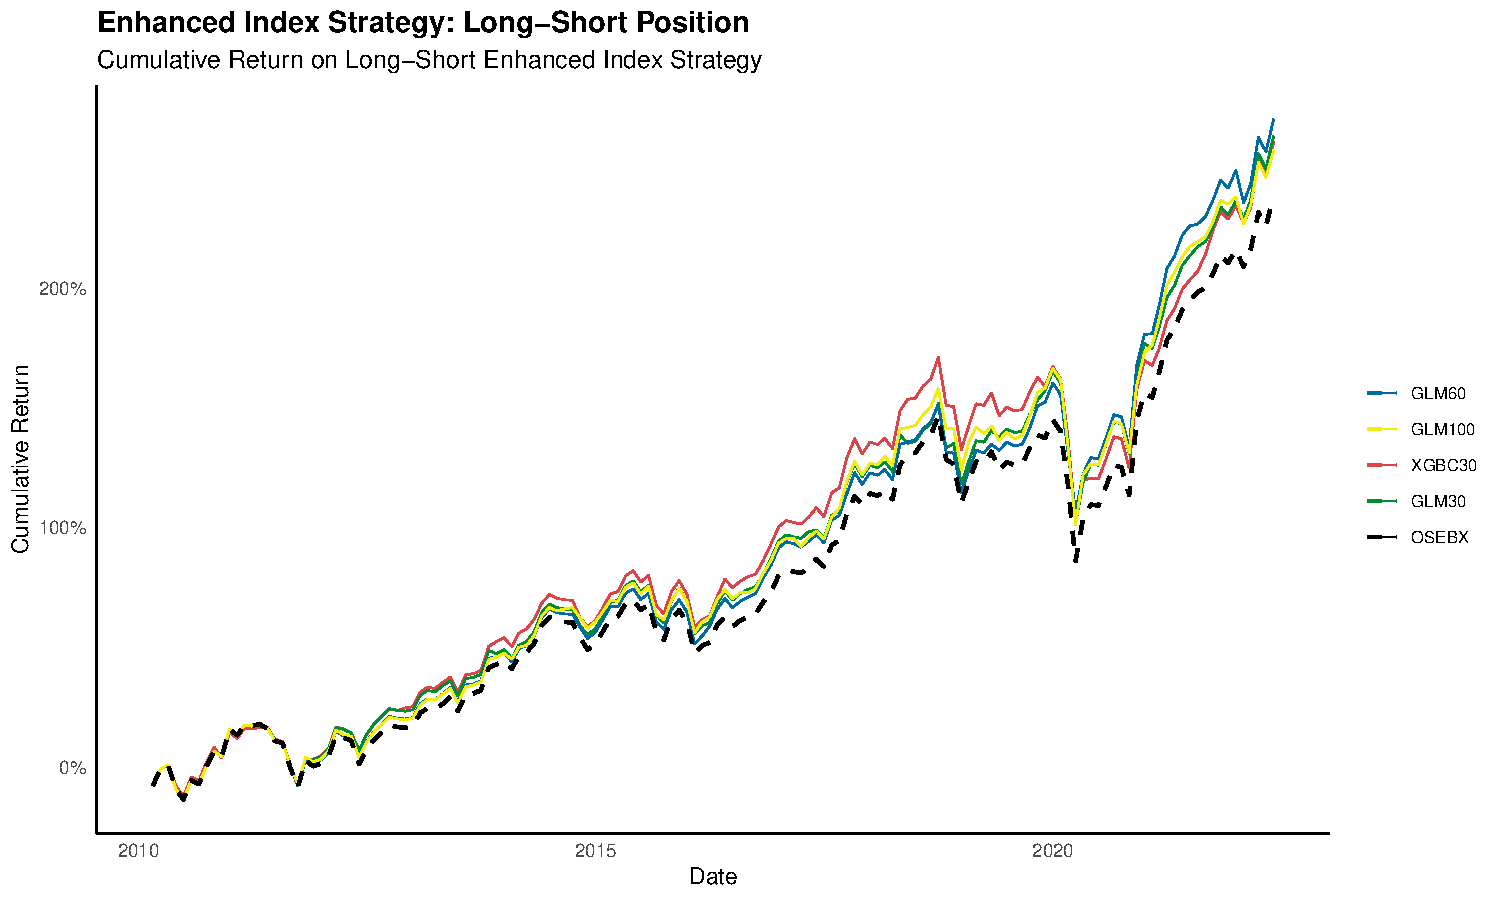
\includegraphics[width=0.9\textwidth]{images/enhanced_long_short.pdf}
    \caption{{Cumulative Return Long-Short Enhanced Index}}
    \subcaption*{Cumulative return for the enhanced long-short portfolios GLM30, GLM60, GLM100, XGBC30 and OSEBX. Only the XGBC30 portfolio yields a significant alpha in the FF3-regression.
    }
    \label{fig:enhanced-long-short-top-5}
\end{figure}

\begin{figure}[H]
    \centering
    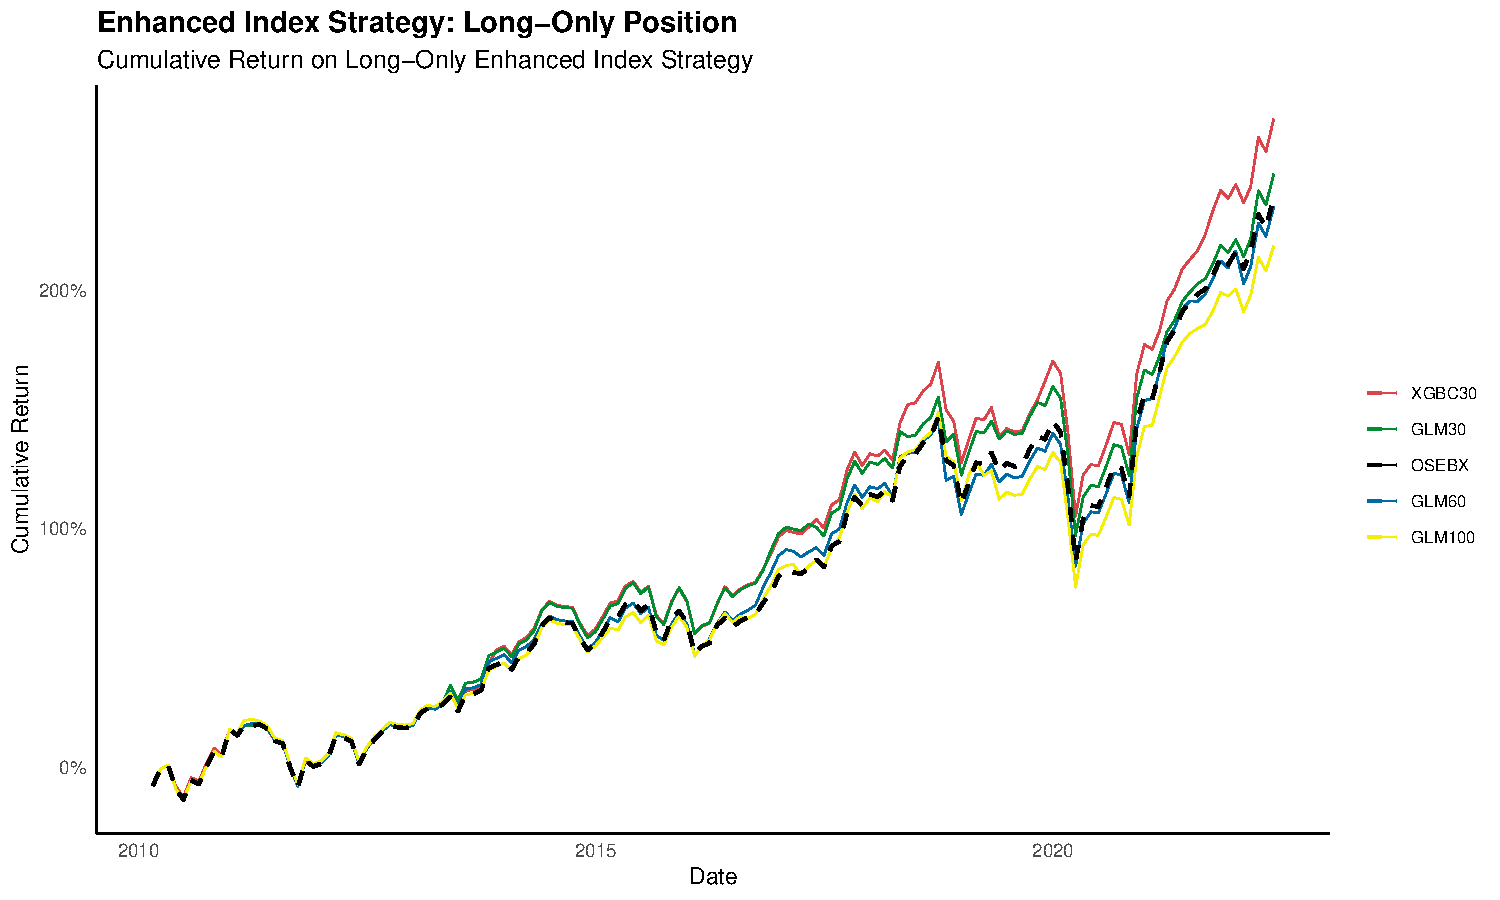
\includegraphics[width=0.9\textwidth]{images/enhanced_long_only.pdf}
    \caption{{Cumulative Return Long-Only Enhanced Index}}
    \subcaption*{Cumulative return for the enhanced long-only portfolios GLM30L, GLM60L, GLM100L, XGBC30L and OSEBX. None of the portfolios yielded significant alphas in the FF3-regression.}
    \label{fig:enhanced-long-only-top-5}
\end{figure}

When considering the visual representation of cumulative return for enhanced portfolios, once again a pattern emerges where the two portfolio types seem to perform well over time. In contrast to the active portfolios analysed in the previous section, the enhanced portfolios are seemingly less exposed to volatility, following OSEBX closely. 

\subsubsection{Conclusion for Research Question (3)}

Finally, our third research question was "To what degree can trading on predicted additions and deletions outperform OSEBX in an enhanced index portfolio?". In this section, we have analysed enhanced index portfolios, which were generated by combining the active trading portfolios from the previous section, with a passive share in OSEBX. The enhanced index portfolios were optimised to have a TE$_{ann}$ of 2\%. In \autoref{tab:CAPM-PERFORMANCE-ENHANCED-INDEX}, we found that several enhanced index portfolios yielded positive CAPM $\alpha_{CAPM}$ and outperformed OSEBX on metrics like $R_p$ and SR. But, in \autoref{fama-french-enhanced-long-short} and \autoref{fama-french-enhanced-long-only}, only the XGBC30 enhanced index portfolio gave a significant FF3 $\alpha_{FF3}$ at a 10\% confidence level after adjusting for risk factors. As expected, when combining the somewhat extreme GLM60 and GLM100 active portfolios with a passive portfolio, we are forced to use a lower active share due to the TE limit of 2\%. In contrast, the risk-averse portfolios allow for a bigger active share, making XGBC30L the highest-yielding enhanced index portfolio. 

In the previous section, we found that one can exploit the index effect by trading on (1) a few accurate predictions, or (2) more changes with a level of risk matching OSEBX. In an enhanced index portfolio, we find that only the latter approach yields significant excess returns in FF3. This is a \textit{key insight} when exploiting the index effect in an enhanced index portfolio. This must come from the fact that GLM can only constitute an active share of 2.8\%$-$4.1\%, compared to XGBC30 at 22.1\%, in an enhanced index portfolio. Finally, we were able to create enhanced index portfolios outperforming OSEBX over the last 13 years, and we conclude that we were able to outperform OSEBX to a reasonable extend.



\newpage
\section{Summary and Conclusions}
\label{Summary and conclusions}

In this thesis, we have investigated the practical application of exploiting the index effect on OSEBX using ML. We did this by using GLM and XGBoost ML models, predicting upcoming changes to OSEBX, by using data variables from Euronext in the OSEBX index methodology. We simulated a portfolio of trading on ML predictions from 2010 to 2023, in both an active trading and enhanced index strategy. Lastly, we analysed the returns from the simulated portfolios.

Our three research questions were to determine (1) "To what degree can machine learning algorithms predict the index composition of OSEBX in the next period?", (2) "To what degree can trading on predicted additions and deletions outperform OSEBX in an active trading portfolio?", and (3) "To what degree can trading on predicted additions and deletions outperform OSEBX in an enhanced index portfolio?". 

(1) We found that it is possible to obtain high accuracy when predicting if a company will be on OSEBX or not in the next period. We obtained more than 95\% accuracy simply by using a lagged variable of the target variable. However, it proved to be more difficult when predicting the actual additions and deletions on OSEBX. By using conditional PPT in XGBoost, we were able to increase the total number of true predicted changes, with the trade-off being lower total accuracy. 

(2) When simulating the active trading portfolios over time, we found that several portfolios were able to outperform OSEBX, both in terms of $R_p$, SR, $\sigma_p$, $\alpha_{CAPM}$ and $\alpha_{FF3}$. In short, both the high-risk high-return GLM100 and GLM60 models, and the lower-risk XGBC30 model were able to create excess returns compared to OSEBX. The key insight is that our findings suggest that the index effect can be exploited by two different approaches. We also point out that the introduction of the conditional PPT in the XGBoost Custom models seems to have served its purpose, as the XGBC30 model proved to be significantly less volatile (yet yielding formidable returns) than the competing GLM portfolios.

(3) Lastly, we also found that trading on recommendations from ML models was able to outperform OSEBX in enhanced index portfolios, even when operating within an annual TE of 2\%. The GLM portfolios gave tiny active shares in the enhanced index portfolio, because of their volatile nature. On the other hand, the XGBC30 enhanced index portfolio still performed well and was the only portfolio able to generate alpha in FF3 within a 10\% confidence level. 

Moreover, we would like to draw a more general conclusion based on our findings in this thesis. Assuming we were able to outperform OSEBX, we want to point out the effect of applying machine learning in practice. We have, as mentioned several times throughout this thesis, found that accuracy is not necessarily the ultimate measurement of assessing model performance. We have in our case shown several times that even the least accurate models can create the most diversified and high-yielding portfolios. The conclusions drawn from this work do therefore come down to the following: one should clearly understand the problem objective before making a predictive ML model. This can in turn broaden the horizon to which one can apply machine learning. If we in this thesis had gone with the model showing the highest accuracy, we would not have been able to exploit anything - because that model predicted no additions nor deletions to OSEBX at all.

\subsection{Robustness of Findings}

In this thesis, we made several assumptions regarding finance and methodology. As with any findings, the performance is dependent on underlying assumptions. 
Regarding our findings in the first research question, the robustness will depend on several factors, including the quality of the data set and our understanding of the official OSEBX rule book. In practice, we faced several missing values in the data set, where we then decided to delete the row rather than trying to find the exact data point. Deleting rows from the data frame can in turn decrease robustness, which creates for a weakness in our data set and models.

When it comes to the second and third research questions, there are also several factors to consider. The first one is the financial assumptions made throughout this thesis. We have, as far as we could, tried to use assumptions that mirror real-world trading. There is no doubt that changing the financial assumptions will affect the results presented in this thesis, and whether or not the assumptions represent real-world trading is open for debate. Also, the FF3 regressions come with some setbacks. Firstly, we have used risk factors that do not specifically represent the exact market we defined. This can cause misleading regression results, and the results should be interpreted carefully. Furthermore, we point out that by using only three risk factors, we are not necessarily capturing the entire risk picture. We could have used several more risk factors in our regressions, but due to the lack of available factors in the Norwegian market, we only used the FF3 model with 3 factors. This is therefore another weakness in our findings. 

Regarding the portfolio simulations, we are also facing some issues challenging the robustness. This is mainly due to missing data in the VWAP data frame. When running the simulations, we have gathered data from this data frame to simulate the portfolio development. Several times we have experienced issues with companies (especially in 2010 and 2011) lacking VWAP. This is a limitation to the simulations, as we then have been forced to drop those predictions from the simulations.

Furthermore, we optimised the enhanced index strategy for TE$_{ann}$ at 2\%. This is in the upper range for accepted TE for an enhanced index fund. In the enhanced index strategy, a lower TE would in turn mean lower excess returns. 

\subsection{Practical Recommendations}

Practically, one can go further in optimising the trading strategy discussed in \autoref{Results and discussion}, which we have not done in this thesis. Possible improvements can be made for (1) time horizon, (2) $\varepsilon$ in the conditional PPT, (3) hyper-parameter tuning, and (4) weighting of the different securities in the portfolios. In sum, trading on the index effect using ML may be optimised further. Despite this, we conclude that our portfolio simulation shows high performance, while still maintaining a low degree of manual intervention and a high degree of repeatability. 


\subsection{Further Research}

Furthermore, this thesis indicates that there \textit{may} be somewhat of a market inefficiency, surrounding the index rebalancing events on OSEBX. We argue that the addition or deletion of a stock does not change the immediate underlying value of the company, so if EMH holds, we should not have been able to exploit the index effect. Therefore it would be of great interest to know if the index effect is a current phenomenon on OSEBX, or if it will continue to exist in the future with more and more investors being aware of it. To fully understand the index effect, one should therefore investigate other indices, which differ from OSEBX in both market size and maturity. 





\newpage

\printbibliography[heading=bibintoc]
\newpage


%\appendix
%\appendix

% \renewcommand{\thesection}{Appendix \Alph{section}}
% Use section* to create an unnumbered section for "Appendix"
% Change subsection numbering
%\section{Appendix}
% \renewcommand{\thesection}{Appendix \arabic{section}}

% \begin{appendices}
% \section{Appendix}  
% \renewcommand{\thesubsection}{Appendix\arabic{subsection}}  

%\begin{appendices}
%\renewcommand{\thesubsection}{A\arabic{subsection}}

%\usepackage[toc,page]{appendix}

\begin{appendices}





\section{Abbreviations and their explanations}
\label{APPENDIX-Abbreviations-and-their-explanations}

%\begin{longtable}{lp{0.7\columnwidth}}
%\caption{Abbreviations and their explanations} 
%\label{abbreviations-and-explanations} 
%\\
%\toprule
%ABBR & Explanations \\ 
%\midrule
%\endfirsthead
%\multicolumn{2}{c}%
%{{\tablename\ \thetable{} -- continued from previous page}} \\
%\toprule
%ABBR & Explanations \\
%\midrule
%\endhead
%\midrule \multicolumn{2}{r}{{Continued on next page}} \\ \bottomrule
%\endfoot
%\bottomrule
%\endlastfoot
%AD & Announcement date\\ 
%AI & Artificial Intelligence \\
%API & Application Programming Interface \\
%AUM & Assets Under Management \\
%AUROC & Area Under Receiver Operating Characteristic \\
%BBG & Bloomberg \\
%CAPM & Capital Asset Pricing Model \\
%CD & Cut-off date \\
%EMH & Efficient Market Hypothesis \\
%EOB & Electronic Order Book \\
%FF & Free Float Market Cap \\
%FF3 & Fama-French 3 Factor Model \\
%FN & False Negative \\
%FP & False Positive \\
%FTSE & Financial Times Stock Exchange \\
%GICS & Global Industry Classification Standard \\
%GLM & Generalised Linear Model \\
%HML & High Minus Low \\
%ICB & Industry Classification Benchmark \\
%IR & Information Ratio \\
%LLM & Large Language Model \\
%ML & Machine Learning \\
%NBIM & Norges Bank Investment Management\\ 
%NHH & Norwegian School of Economics\\
%OLS & Ordinary Least Squares \\
%OSE & Oslo Stock Exchange \\
%OSEAX & Oslo Stock Exchange All Shares Index\\
%OSEBX & Oslo Stock Exchange Benchmark Index\\
%PPT & Posterior Probability Threshold \\
%RF & Random Forest \\
%RL & Reinforcement Learning \\
%ROC & Receiver Operating Characteristic \\
%SL & Supervised Learning \\
%SMB & Small Minus Big \\
%SR & Sharpe Ratio \\
%TE & Tracking Error \\
%TN & True Negative \\
%TO & Turnover Electronic Order Book \\
%TP & True Positive \\
%TS & Trading Status \\
%TSCV & Time Series Cross-Validation \\
%UL & Unsupervised Learning \\
%VIP & Variance Importance Plot \\
%VWAP & Volume Weighted Average Price\\
%XGBB & XGBoost Benchmark \\
%XGBC & XGBoost Custom \\
%XGBoost & eXtreme Gradient Boosting \\
%\end{longtable}





\vspace{-1em}
\begin{table}[H]
\centering
\footnotesize
\begin{tabularx}{\textwidth}{ll}
\hline
ABBR & Explanation \\ 
\hline
AD & Announcement date\\ 
AI & Artificial Intelligence \\
API & Application Programming Interface \\
AUM & Assets Under Management \\
AUROC & Area Under Receiver Operating Characteristic \\
BBG & Bloomberg \\
CAPM & Capital Asset Pricing Model \\
CD & Cut-off date \\
EMH & Efficient Market Hypothesis \\
EOB & Electronic Order Book \\
FF & Free Float Market Cap \\
FF3 & Fama-French 3 Factor Model \\
FN & False Negative \\
FP & False Positive \\
FTSE & Financial Times Stock Exchange \\
GICS & Global Industry Classification Standard \\
GLM & Generalised Linear Model \\
HML & High Minus Low \\
ICB & Industry Classification Benchmark \\
IR & Information Ratio \\
LLM & Large Language Model \\
ML & Machine Learning \\
NBIM & Norges Bank Investment Management\\ 
NHH & Norwegian School of Economics\\
OLS & Ordinary Least Squares \\
OSE & Oslo Stock Exchange \\
OSEAX & Oslo Stock Exchange All Shares Index\\
OSEBX & Oslo Stock Exchange Benchmark Index\\
PPT & Posterior Probability Threshold \\
RF & Random Forest \\
RL & Reinforcement Learning \\
ROC & Receiver Operating Characteristic \\
SL & Supervised Learning \\
SMB & Small Minus Big \\
SR & Sharpe Ratio \\
TE & Tracking Error \\
TN & True Negative \\
TO & Turnover Electronic Order Book \\
TP & True Positive \\
TS & Trading Status \\
TSCV & Time Series Cross-Validation \\
UL & Unsupervised Learning \\
VIP & Variance Importance Plot \\
VWAP & Volume Weighted Average Price\\
XGBB & XGBoost Benchmark \\
XGBC & XGBoost Custom \\
XGBoost & eXtreme Gradient Boosting \\
\hline
\end{tabularx}
\vspace{1em}
\caption{Abbriviation}
\label{from-gics-to-icb}
\end{table}



\section{OSEBX Constituents Since 2006}
\label{APPENDIX-OSEBX-constituents-at-the-start-of-2006}
\begin{table}[H]
\centering
\footnotesize
\begin{tabularx}\textwidth{lll}
\toprule
OSEBX constituents at the start of 2006   \\ 
\midrule
ABG Sundal Collier Holding ASA & Ekornes ASA & Otello Corp ASA \\
Akastor ASA & Eltek AS & PGS ASA \\
Aker ASA & Equinor ASA & PRA Group Europe AS \\
Andvord Tybring-Gjedde & Expert AS & PhotoCure ASA \\
Arribatec Group ASA & Frontline PLC & Profdoc AS \\
Atea ASA & Funcom Se & Prosafe SE \\
Axactor ASA & Hafslund ASA & Q-Free ASA \\
BW Gas AS & Jason Shipping AS & Royal Caribbean Cruises Ltd \\
BWG Homes ASA & Kongsberg Automotive ASA & STX Europe AS \\
Carasent ASA & Leroy Seafood Group ASA & SUBSEA 7 Inc \\
Cermaq Group AS & Magnora ASA & Schibsted ASA \\
Crew Gold Corp & Microsoft Dev Center Norway AS & Seadrill Ltd/old \\
DNB Bank ASA & Mowi ASA & Sinvest ASA \\
DNO ASA & NEL ASA & Stolt-Nielsen Ltd \\
Dolphin Drilling ASA & Nera ASA & Storebrand ASA \\
Norsk Hydro ASA & Ocean RIG ASA & Subsea 7 SA \\
Norwegian Air Shuttle ASA & Odfjell SE & SuperOffice AS \\
NorGani Hotels ASA & Odfjell SE & TGS ASA \\
Origio A/S & Orkla ASA & TOMRA Systems ASA \\
Tandberg AS & Tandberg Television ASA & Techstep ASA \\
Telenor ASA & Veidekke ASA & Wilh Wilhelmsen Holding ASA \\
Wilh Wilhelmsen Holding ASA & Yara International ASA &  \\
\bottomrule
\end{tabularx}

\vspace{1em}
\caption{OSEBX constituents at the start of 2006}
\subcaption*{This table shows all companies composing OSEBX in 2006, which is what our data covers.}
\label{osebx-constituents-start-of-2006}
\end{table}


\section{OSEBX changes since 2006}
% new long table for changes
\begin{table}[H]
\centering
\scriptsize
\begin{tabular}{lll}
  \hline
Company & Additions & Deletions \\  
\hline
ABG Sundal Collier Holding ASA & 2020-05-29 & 2016-11-30 \\
AF Gruppen ASA & 2013-05-31 & \\
AMSC ASA & 2019-05-31, 2016-11-30, 2014-05-30 & 2021-03-19, 2017-05-31, 2016-05-31 \\
Akastor ASA & 2015-05-29 & \\
Aker ASA & 2011-11-30, 2009-11-30 & 2010-05-31, 2009-05-29 \\
Aker BP ASA & 2012-05-31 & \\
Aker BioMarine ASA & 2011-05-31, 2007-06-29 & 2011-11-30, 2007-12-30 \\
Aker Carbon Capture ASA & 2023-03-17, 2022-03-18 & 2022-09-16 \\
Aker Horizons ASA & 2021-09-17 & \\
Aker Solutions ASA & 2016-11-30 & 2016-05-31 \\
Algeta ASA & 2009-11-30 & \\
Altinex AS & 2006-12-29 & \\
Archer Ltd & 2011-05-31 & 2011-11-30 \\
ArcticZymes Technologies ASA & 2021-03-19, 2014-05-30 & 2017-05-31 \\
Arendals Fossekompani ASA & 2022-03-18 & \\
Arribatec Group ASA & 2011-11-30 & \\
Asetek A/S & 2016-11-30 & 2021-03-19, 2014-11-28 \\
Austevoll Seafood ASA & 2018-05-31, 2007-06-29 & 2020-05-29, 2013-11-29 \\
AutoStore Holdings Ltd & 2022-03-18 & \\
Avance Gas Holding Ltd & 2020-05-29, 2015-05-29 & 2022-03-18, 2016-11-30 \\
Axactor ASA & 2016-05-31 & 2021-09-17, 2007-06-29 \\
Axel Springer Norway AS & 2006-12-29 & \\
BW Gas AS & 2007-06-29 & \\
BW LPG Ltd & 2017-11-30, 2014-05-30 & 2016-11-30 \\
BW Offshore Ltd & 2018-05-31, 2010-11-30, 2007-06-29 & 2021-03-19, 2011-05-31, 2008-06-30 \\
BWG Homes ASA & 2009-05-29 & 2008-12-30 \\
Bakkafrost P/F & 2014-05-30, 2011-11-30 & 2013-05-31, 2010-11-30 \\
Bank Norwegian ASA & 2017-11-30, 2016-11-30 & 2017-05-31 \\
Bergenbio ASA & 2018-05-31 & 2023-03-17 \\
Bonheur ASA & 2019-11-29 & \\
Borr Drilling Ltd & 2023-03-17, 2017-11-30 & 2020-05-29 \\
Borregaard ASA & 2021-03-19 & \\
Bouvet ASA & 2020-05-29 & \\
COSL Holding AS & 2006-12-29 & \\
Cadeler A/S & 2022-09-16 & \\
Carasent ASA & 2021-03-19 & 2023-03-17, 2007-12-30 \\
Cermaq Group AS & 2014-05-30 & \\
Circio Holding ASA & 2017-11-30 & 2018-11-30 \\
Cloudberry Clean Energy ASA & 2022-03-18 & \\
Copeinca ASA & 2009-11-30, 2007-12-30 & 2010-05-31, 2008-12-30 \\
Crayon Group Holding ASA & 2020-05-29 & \\
Crew Gold Corp & 2007-06-29 & \\
Data Respons ASA & 2019-11-29, 2006-12-29 & 2009-11-30 \\
Dolphin Drilling ASA & 2015-11-30 & \\
Electromagnetic Geoservices ASA & 2012-11-30 & 2013-11-29 \\
Elkem ASA & 2019-05-31 & \\
Elmera Group ASA & 2019-05-31 & \\
Eltek AS & 2010-05-31 & 2008-12-30 \\
Ensurge Micropower ASA & 2015-05-29 & 2019-05-31 \\
Europris ASA & 2015-11-30 & \\
Evry AS & 2017-11-30 & \\
FLEX LNG Ltd & 2021-09-17 & \\
Fjord1 AS & 2018-05-31 & 2021-03-19 \\
Frontline PLC & 2015-05-29 & 2013-05-31 \\
Funcom Se & 2017-11-30, 2012-05-31 & 2018-11-30, 2012-11-30, 2008-12-30 \\
Gaming Innovation Group Inc & 2021-09-17, 2017-05-31, 2016-05-31 & 2022-09-16, 2021-03-19, 2016-11-30 \\
Gjensidige Forsikring ASA & 2011-05-31 & \\
Golden Ocean Group Ltd/Old & 2006-12-29 & \\
Grieg Seafood ASA & 2017-05-31 & 2021-09-17 \\
Hafnia Ltd & 2022-09-16 & \\
Hafslund ASA & 2016-11-30, 2006-12-29 & 2013-11-29, 2009-05-29 \\
Hexagon Composites ASA & 2019-05-31, 2016-05-31, 2014-05-30 & 2018-11-30, 2014-11-28 \\
IDEX Biometrics ASA & 2015-05-29 & 2021-09-17 \\
IMAREX ASA & 2007-12-30 & 2009-11-30 \\
Itera ASA & 2007-06-29 & 2008-06-30 \\ 
    \midrule \multicolumn{l}{r}{{Continued on next page}} \\
   \hline
\end{tabular}   
\end{table}

\newpage
% new long table for changes
\begin{table}[H]
\centering
\scriptsize
\begin{tabularx}\textwidth{lll}
    \midrule \multicolumn{l}{r}{{Continuation from previous page}} \\

  \hline
Company & Additions & Deletions \\  
\hline
Jason Shipping AS & 2007-12-30 & 2009-05-29, 2007-06-29 \\
Jinhui Shipping \& Transportation Ltd & 2010-11-30, 2007-06-29 & 2011-05-31, 2008-12-30 \\
Kahoot! ASA & 2021-09-17 & \\
Karo Pharma Norge AS & 2014-11-28, 2010-05-31 & 2013-05-31 \\
Kid ASA & 2021-03-19 & \\
Kitron ASA & 2016-11-30 & \\
Komplett ASA & 2006-12-29 & 2008-12-30 \\
Kongsberg Gruppen ASA & 2010-05-31, 2008-06-30 & 2009-11-30 \\
Leroy Seafood Group ASA & 2016-11-30, 2009-11-30 & 2014-11-28, 2009-05-29 \\
Link Mobility Group ASA & 2017-05-31 & \\
MPC Container Ships ASA & 2018-11-30 & \\
Magnora ASA & 2012-05-31 & \\
Mamut AS & 2007-06-29 & 2010-05-31 \\
Medistim ASA & 2020-05-29 & 2021-09-17 \\
Morpol ASA & 2010-11-30 & 2012-05-31 \\
Multiconsult ASA & 2021-09-17, 2015-11-30 & 2023-03-17, 2017-05-31 \\
NEL ASA & 2018-05-31 & 2007-12-30 \\
NRC Group ASA & 2007-06-29 & 2010-05-31 \\
Next Biometrics Group AS & 2016-05-31 & 2019-11-29 \\
Nordic Semiconductor ASA & 2010-05-31, 2007-12-30 & 2008-12-30 \\
Norwegian Property ASA & 2018-05-31 & \\
Nykode Therapeutics ASA & 2022-09-16 & \\
Odfjell SE & 2010-05-31, 2008-06-30 & 2014-05-30, 2009-05-29, 2008-12-30, 2007-12-30 \\
Olav Thon Eiendomsselskap ASA & 2013-05-31, 2008-06-30, 2006-12-29 & 2021-03-19, 2008-12-30, 2007-06-29 \\
Origio A/S & 2007-12-30 & 2009-11-30, 2007-06-29 \\
Otello Corp ASA & 2018-11-30 & \\
PA Resources AB & 2006-12-29 & 2008-12-30 \\
PCI Biotech Holding ASA & 2018-05-31 & 2022-03-18 \\
PGS ASA & 2023-03-17 & 2021-03-19 \\
PRA Group Europe AS & 2011-11-30 & 2012-05-31, 2010-11-30 \\
Pexip Holding ASA & 2021-03-19 & 2022-09-16 \\
PhotoCure ASA & 2015-05-29, 2014-05-30, 2010-05-31 & 2014-11-28, 2012-11-30, 2008-12-30 \\
Polarcus Ltd & 2013-05-31 & 2014-05-30 \\
Prosafe SE & 2016-05-31 & \\
Q-Free ASA & 2015-05-29, 2010-05-31 & 2016-11-30, 2014-11-28, 2006-12-29 \\
Questerre Energy Corp & 2017-11-30, 2010-05-31 & 2018-11-30, 2011-11-30, 2009-11-30 \\
REC Silicon ASA & 2021-03-19 & 2019-11-29 \\
RenoNorden ASA & 2015-05-29 & 2015-11-30 \\
Rieber & Son AS & 2006-12-29 & 2007-06-29 \\
SAS AB & 2016-05-31 & 2016-11-30 \\
SATS ASA & 2020-05-29 & 2023-03-17 \\
Salmar ASA & 2013-11-29, 2007-12-30 & 2013-05-31 \\
Schibsted ASA & 2015-11-30 & \\
Seadrill Ltd/old & 2018-05-31 & \\
Sinvest ASA & 2006-12-29 & \\
Solon Eiendom ASA & 2010-05-31 & 2015-05-29 \\
Songa Offshore SE & 2012-11-30, 2009-11-30, 2007-12-30 & 2013-05-31, 2011-05-31, 2008-12-30 \\
SpareBank 1 SR-Bank ASA & 2017-05-31 & \\
Steen \& Stroem AS & 2007-06-29 & \\
StrongPoint ASA & 2009-05-29 & 2009-11-30 \\
Team Tankers Management Holding AS & 2010-05-31, 2007-06-29 & 2010-11-30, 2009-05-29 \\
Techstep ASA & 2008-12-30 & \\
Teekay Petrojarl AS & 2006-12-29 & \\
Thor Medical ASA & 2015-05-29 & 2022-09-16 \\
TietoEVRY Oyj & 2020-05-29 & 2021-03-19 \\
Treasure ASA & 2016-11-30 & 2018-05-31 \\
Tribona ASA & 2007-12-30 & 2008-12-30 \\
Ultimovacs ASA & 2021-09-17 & \\
Var Energi ASA & 2022-09-16 & \\
Veidekke ASA & 2012-05-31, 2009-11-30, 2008-06-30 & 2010-05-31, 2008-12-30, 2007-12-30 \\
Visolit AS & 2006-12-29 & 2007-06-29 \\
Vizrt Ltd & 2006-12-29 & 2011-05-31 \\
Vow ASA & 2021-03-19 & 2022-03-18 \\
Wallenius Wilhelmsen ASA & 2010-11-30 & \\
Wavefield Inseis AS & 2007-06-29 & 2008-12-30 \\
Wilh Wilhelmsen Holding ASA & 2011-11-30 & 2020-05-29, 2018-11-30, 2008-12-30 \\
XXL ASA &  & 2022-03-18 \\
   \hline
\end{tabularx}   
\vspace{1em}
\caption{All OSEBX Additions and Deletions since 2006}
\subcaption*{All changes to OSEBX in the period we are analysing in this thesis.}

\end{table}




\section{CD, AD, and ED from 2006 to 2023}
\label{APPENDIX CD, AD, and ED from 2006 to 2023}
\begin{table}[H]
\centering
\vspace{1em}
\label{CD-AD-ED-2006-2023}
\begin{minipage}{.5\textwidth}
\centering
\begin{tabular}{llll}
\hline
 & CD & AD & ED \\ 
\hline
1 & 2023-02-17 & 2023-03-08 & 2023-03-17 \\ 
2 & 2022-08-19 & 2022-09-07 & 2022-09-16 \\ 
3 & 2022-02-18 & 2022-03-09 & 2022-03-18 \\ 
4 & 2021-08-20 & 2021-09-08 & 2021-09-17 \\ 
5 & 2021-02-19 & 2021-03-10 & 2021-03-19 \\ 
6 & 2020-04-30 & 2020-05-12 & 2020-05-29 \\ 
7 & 2019-11-01 & 2019-11-08 & 2019-11-29 \\ 
8 & 2019-05-03 & 2019-05-09 & 2019-05-31 \\ 
9 & 2018-11-02 & 2018-11-09 & 2018-11-30 \\ 
10 & 2018-05-03 & 2018-05-09 & 2018-05-31 \\ 
11 & 2017-11-02 & 2017-11-10 & 2017-11-30 \\ 
12 & 2017-05-03 & 2017-05-05 & 2017-05-31 \\ 
13 & 2016-11-02 & 2016-11-10 & 2016-11-30 \\ 
14 & 2016-05-03 & 2016-05-12 & 2016-05-31 \\ 
15 & 2015-11-02 & 2015-11-12 & 2015-11-30 \\ 
16 & 2015-04-30 & 2015-05-13 & 2015-05-29 \\ 
17 & 2014-10-31 & 2014-11-13 & 2014-11-28 \\ 
\hline
\end{tabular}
\end{minipage}%
\begin{minipage}{.5\textwidth}
\centering
\begin{tabular}{llll}
\hline
 & CD & AD & ED \\ 
\hline 
18 & 2014-05-02 & 2014-05-15 & 2014-05-30 \\ 
19 & 2013-11-01 & 2013-11-14 & 2013-11-29 \\ 
20 & 2013-05-03 & 2013-05-14 & 2013-05-31 \\ 
21 & 2012-11-02 & 2012-11-16 & 2012-11-30 \\ 
22 & 2012-05-03 & 2012-05-16 & 2012-05-31 \\ 
23 & 2011-11-02 & 2011-11-11 & 2011-11-30 \\ 
24 & 2011-05-03 & 2011-05-12 & 2011-05-31 \\ 
25 & 2010-11-02 & 2010-11-15 & 2010-11-30 \\ 
26 & 2010-05-03 & 2010-05-12 & 2010-05-31 \\ 
27 & 2009-11-02 & 2009-11-13 & 2009-11-30 \\ 
28 & 2009-04-30 & 2009-05-14 & 2009-05-29 \\ 
29 & 2008-12-02 & 2008-12-11 & 2008-12-30 \\ 
30 & 2008-06-02 & 2008-06-05 & 2008-06-30 \\ 
31 & 2007-11-30 & 2007-12-04 & 2007-12-30 \\ 
32 & 2007-06-01 & 2007-06-08 & 2007-06-29 \\ 
33 & 2006-12-01 & 2006-12-04 & 2006-12-29 \\ 
34 & 2006-06-02 & 2006-06-08 & 2006-06-30 \\ 
\hline
\end{tabular}
\end{minipage}
\vspace{1em}
\caption{CD, AD, and ED from 2006 to 2023}
\subcaption*{A summary of all important dates since 2006. }
\end{table}









\section{ICB Estimations}
\label{APPENDIX From GICS to ICB}
\vspace{-1em}
\begin{table}[H]
\centering
\footnotesize
\begin{tabularx}{\textwidth}{lXXX}
\hline
 & ticker & company & ICB (estimated) \\ 
\hline
1 & 1643322D NO Equity & Seadrill Ltd/old & Energy \\ 
2 & EDRILL NO Equity & Seadrill X ASA & Energy \\ 
3 & ALX NO Equity & Altinex AS & Energy \\ 
4 & SIN NO Equity & Sinvest ASA & Energy \\ 
5 & 8185832Q NO Equity & Aker Drilling ASA/Old & Energy \\ 
6 & APL NO Equity & APL ASA & Energy \\ 
7 & FRID NO Equity & Saipem Discoverer Invest SARL & Energy \\ 
8 & APLC NO Equity & APL Advanced Production \& Loading PLC & Energy \\ 
9 & NOV NO Equity & Norsk Vekst AS & Financial Services \\ 
10 & FSL NO Equity & Fesil AS & Industrial Goods and Services \\ 
11 & GAS NO Equity & BW Gas AS & Industrial Goods and Services \\ 
12 & POLI NO Equity & Berry Packaging Norway AS & Industrial Goods and Services \\ 
13 & DESS NO Equity & Deep Sea Supply ASA & Industrial Goods and Services \\ 
14 & BHOC NO Equity & B+H Ocean Carriers Ltd & Industrial Goods and Services \\ 
15 & NEMI NO Equity & Nemi Forsikring AS & Insurance \\ 
16 & PFI NO Equity & P4 Radio Hele Norge AS & Media \\ 
17 & SST NO Equity & Steen \& Stroem AS & Realestate \\ 
18 & ATG NO Equity & Andvord Tybring-Gjedde & Retail \\ 
19 & EXPERT NO Equity & Expert AS & Retail \\ 
20 & CNS NO Equity & Conseptor ASA & Technology \\ 
21 & CSG NO Equity & Component Software Group & Technology \\ 
22 & CAPTU NO Equity & Captura AS & Technology \\ 
23 & ACTIVE NO Equity & Active 24 ASA & Technology \\ 
24 & TAT NO Equity & Tandberg Television ASA & Technology \\ 
25 & NSTAT NO Equity & Norstat ASA & Telecommunications \\ 
26 & NER NO Equity & Nera ASA & Telecommunications \\ 
27 & RIC NO Equity & Rica Hotels ASA & Travel and Leisure \\ 
\hline
\end{tabularx}
\vspace{1em}
\caption{Estimated ICB-sectors}
\subcaption*{Estimated ICB supersectors are estimated for the companies we were unable to obtain this information directly from BBG. }
\label{from-gics-to-icb}
\end{table}


\newpage

\section{XGBoost Hyperparameters}
\label{xgb-hyperparameters}
\begin{table}[H]
\centering
\begin{tabular}{rll}
\toprule
 & parameters & value \\ 
\midrule
1 & nrounds & 50 \\ 
  2 & max\_depth & 1000 \\ 
  3 & objective & \texttt{binary:logistic} \\ 
  4 & remaining & default \\ 
\bottomrule
\end{tabular}
\vspace{1em}
\caption{{XGBoost Hyperparameters}}
\subcaption*{XGBoost shows great flexibility compared to other models in the ability to tune hyperparameters when optimising for specific use cases. Note that these parameters are not optimised to maximise accuracy.}
\end{table}



\section{Excel Bloomberg Add In BQL Formulas}
\label{APPENDIX-Excel-Bloomberg-Add-In-BQL-Formulas}
\begin{table}[H]
\centering
\begin{tabular}{ll}
\hline
Command & Code \\ 
\hline
\texttt{trading\_status} & \begin{minipage}[t]{0.6\textwidth}

\texttt{=@BQL(A2; "(#traded\_days/" \& F2 \& ")*100"; "#px=px\_last(dates=range(" \&@BQL.DATE(D2) \& ","\&@BQL.DATE(E2) \& "))"; "#traded\_days = count(matches( #px,#px!=NA)).value"; "#total\_days=count(#px().date).value")}




\end{minipage} \\
\hline
\texttt{turnover} & \begin{minipage}[t]{0.6\textwidth}

\texttt{
=@BQL(A2;" #tot";"#high=sum(first(group(sort( turnover(dates=range(" \&@BQL.DATE(C2) \& "," \&@BQL.DATE(E2) \& ")),order=desc)),12)), #sum=sum(Group(turnover(dates=range(" \&@BQL.DATE(C2) \& "," \&@BQL.DATE(E2) \& ")))), #tot = #sum - #high")
}

\end{minipage} \\
\hline
\texttt{icb\_supersector} & \begin{minipage}[t]{0.6\textwidth}
\texttt{
=BDP(A2;"icb\_supersector\_name")
}
\end{minipage} \\
\hline
\texttt{free\_float} & \begin{minipage}[t]{0.6\textwidth}
\texttt{
=BDH(A2;"cur\_mkt\_cap";E2)* BDH(A2; "eqy\_free\_float\_pct";E2)%
}


\end{minipage} \\
\hline
\end{tabular}
\vspace{1em}
\caption{Excel BBG Add In BQL Functions}
\subcaption*{A2: ticker, C2: one year before E2, D2: start date trading period, E2: end date trading period, and F2: total trading days.}
\label{excel-bbg-bql}
\end{table}


\section{Descriptive statistics}
\label{APPENDIX-Descriptive-statistics}

\begin{figure}[H]
    \centering
    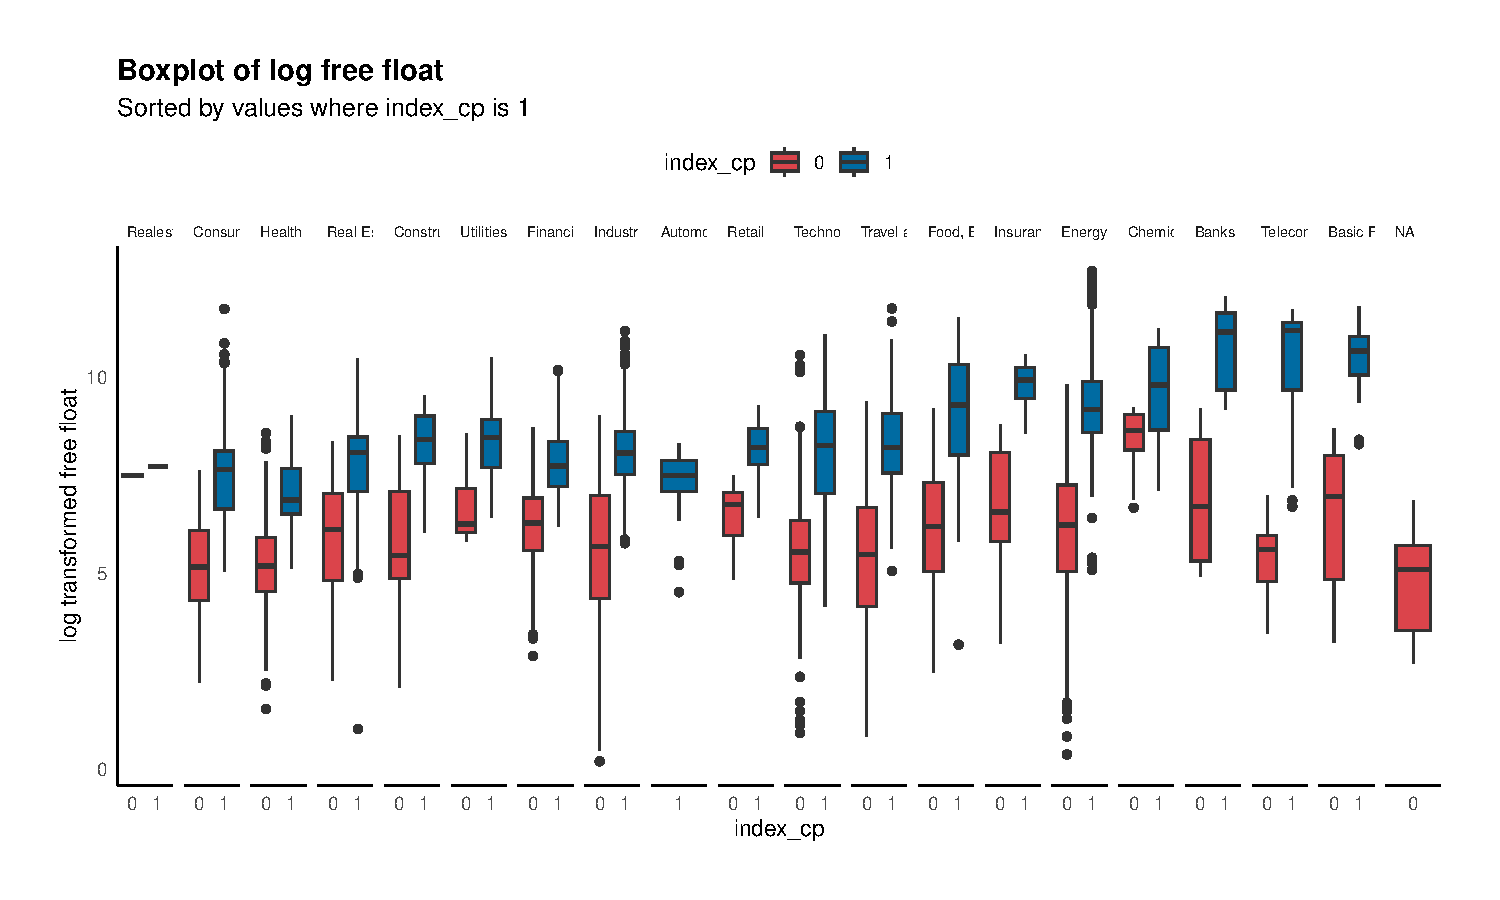
\includegraphics[width=\textwidth]{images/box_free_float.pdf}
    \caption{Box-plot \texttt{free\_float} and \texttt{index\_cp}}
    \subcaption*{Illustration of allocation of \texttt{index\_cp} per different ICB supersector, in relation to the logarithm of \texttt{free\_float}.}
    \label{fig:box_free_float}
\end{figure}

\begin{figure}[H]
    \centering
    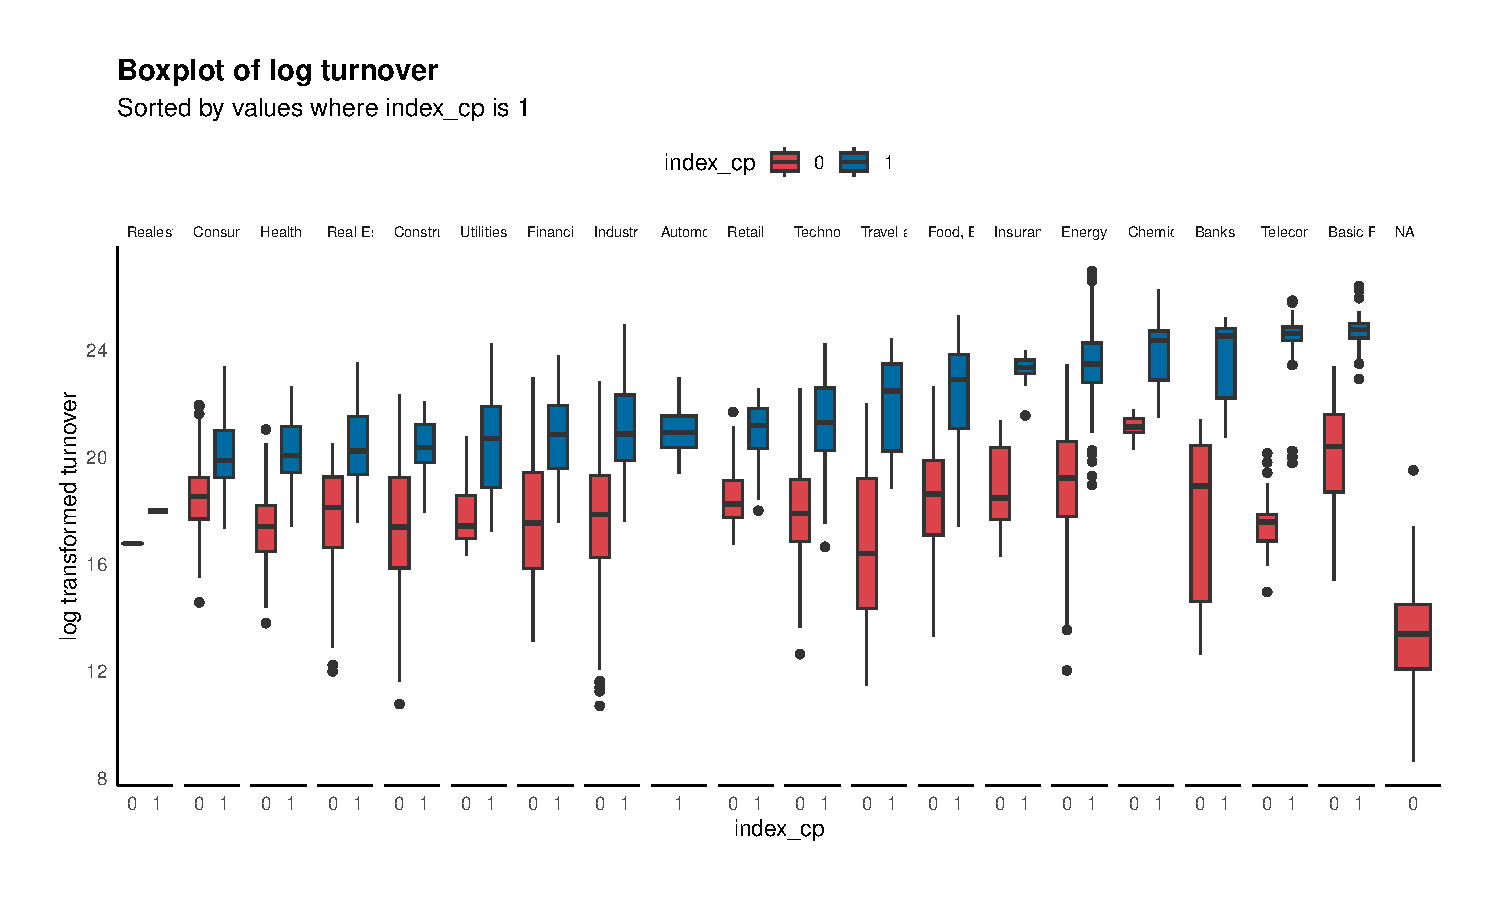
\includegraphics[width=\textwidth]{images/box_turnover.pdf}
    \caption{Box-plot \texttt{turnover\_eob} and \texttt{index\_cp}}
        \subcaption*{Illustration of allocation of \texttt{index\_cp} per different ICB supersector, in relation to the logarithm of \texttt{turnover\_eob}.}
    \label{fig:box_turnover}
\end{figure}

\begin{figure}[H]
    \centering
    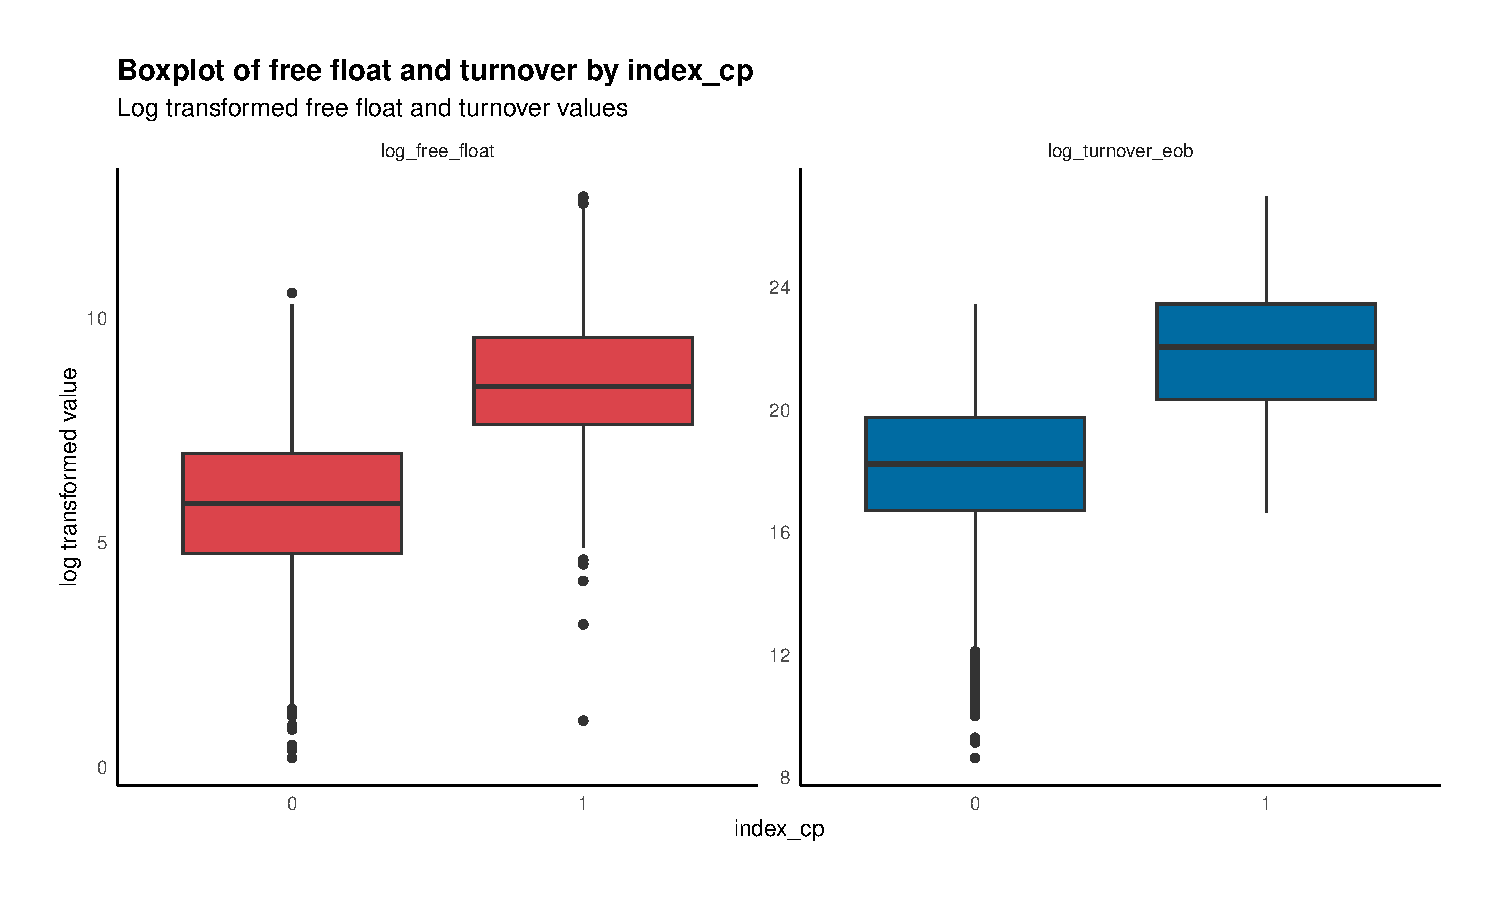
\includegraphics[width=\textwidth]{images/box_facetted.pdf}
    \caption{Box-plot \texttt{turnover\_eob}, \texttt{free\_float}, and \texttt{index\_cp}}
        \subcaption*{Boxplot of \texttt{free\_float} and \texttt{index\_cp}, and \texttt{turnover\_eob} and \texttt{index\_cp} }
    \label{fig:box_facetted}
\end{figure}


\begin{figure}[H]
    \centering
    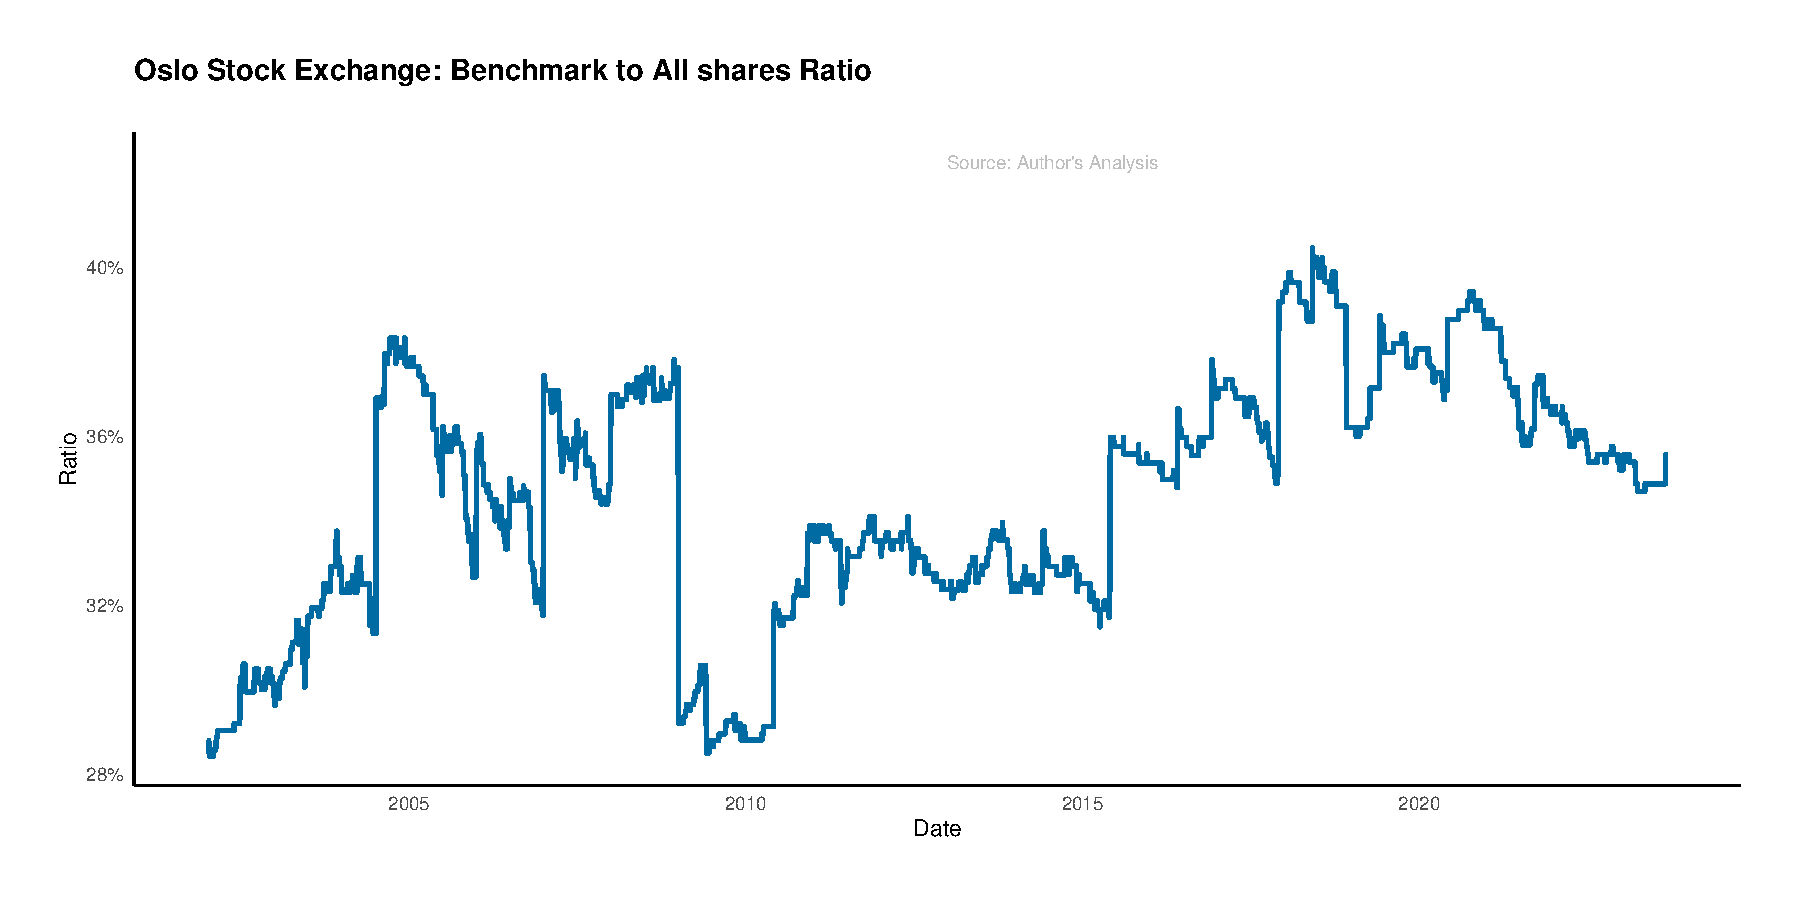
\includegraphics[width=\textwidth]{images/plot_share_126.pdf}
    \caption{Ratio of OSEBX to OSEAX member count}
    \label{Share of Benchmark to All shares over time}
\end{figure}

\begin{figure}[H]
    \centering
    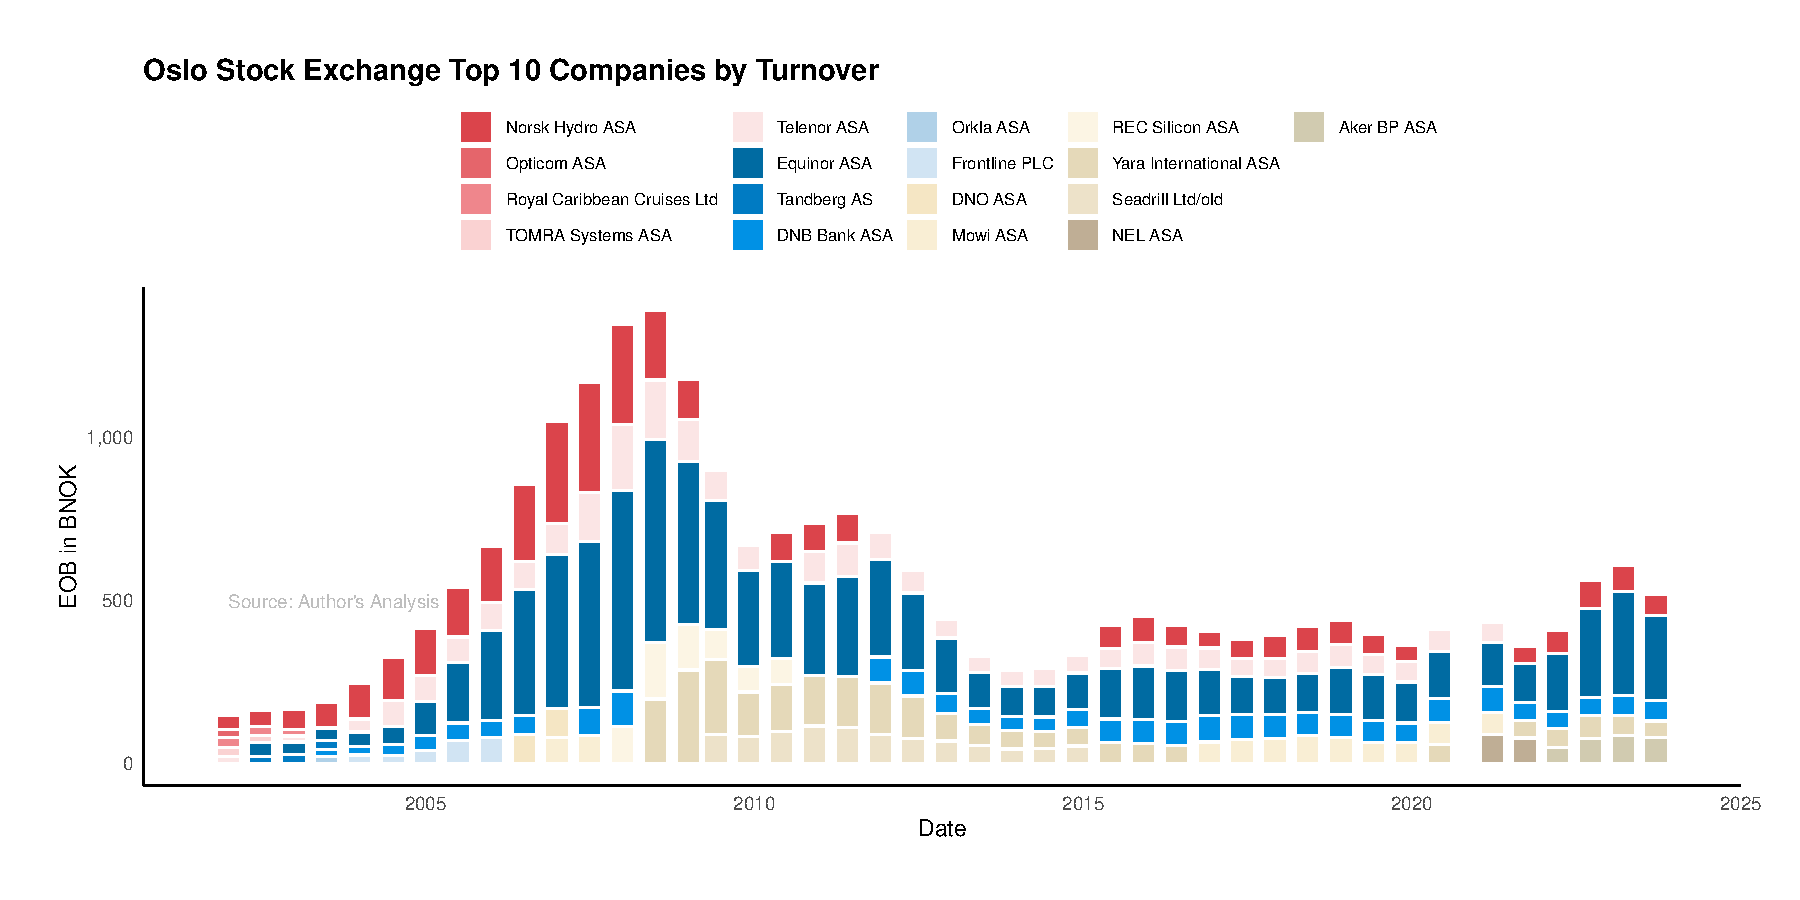
\includegraphics[width=\textwidth]{images/plot_turnover.pdf}
    \caption{Turnover of 10 largest OSEBX companies over time}
    \subcaption*{Turnover of 10 largest OSEBX companies over time, being large Norwegian Companies.}
    \label{OSEBX-top-10-turnover}
\end{figure}

\begin{figure}[H]
    \centering
    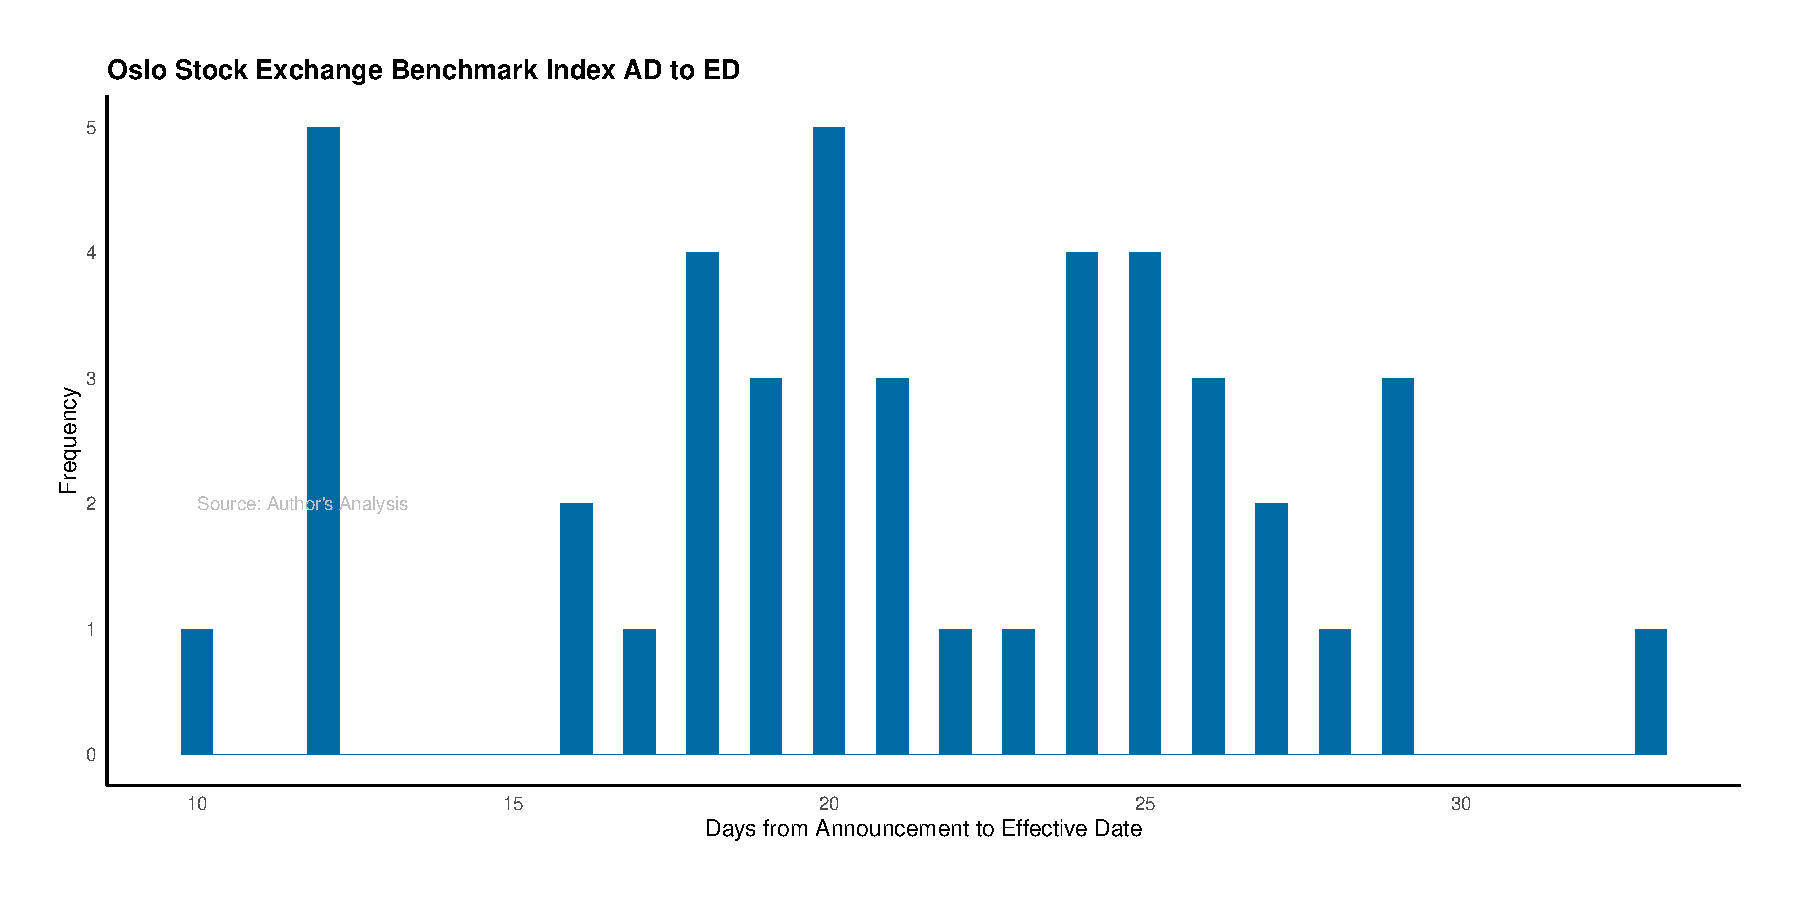
\includegraphics[width=\textwidth]{images/plot_ad_to_ed.pdf}
    \caption{OSEBX number of days from AD to ED}
        \subcaption*{Number of days between each announcement date and effective date illustrated as a histogram. The length varies between 10 and 32 days.}
    \label{OSEBX-ad-to-ed}
\end{figure}

\begin{figure}[H]
    \centering
    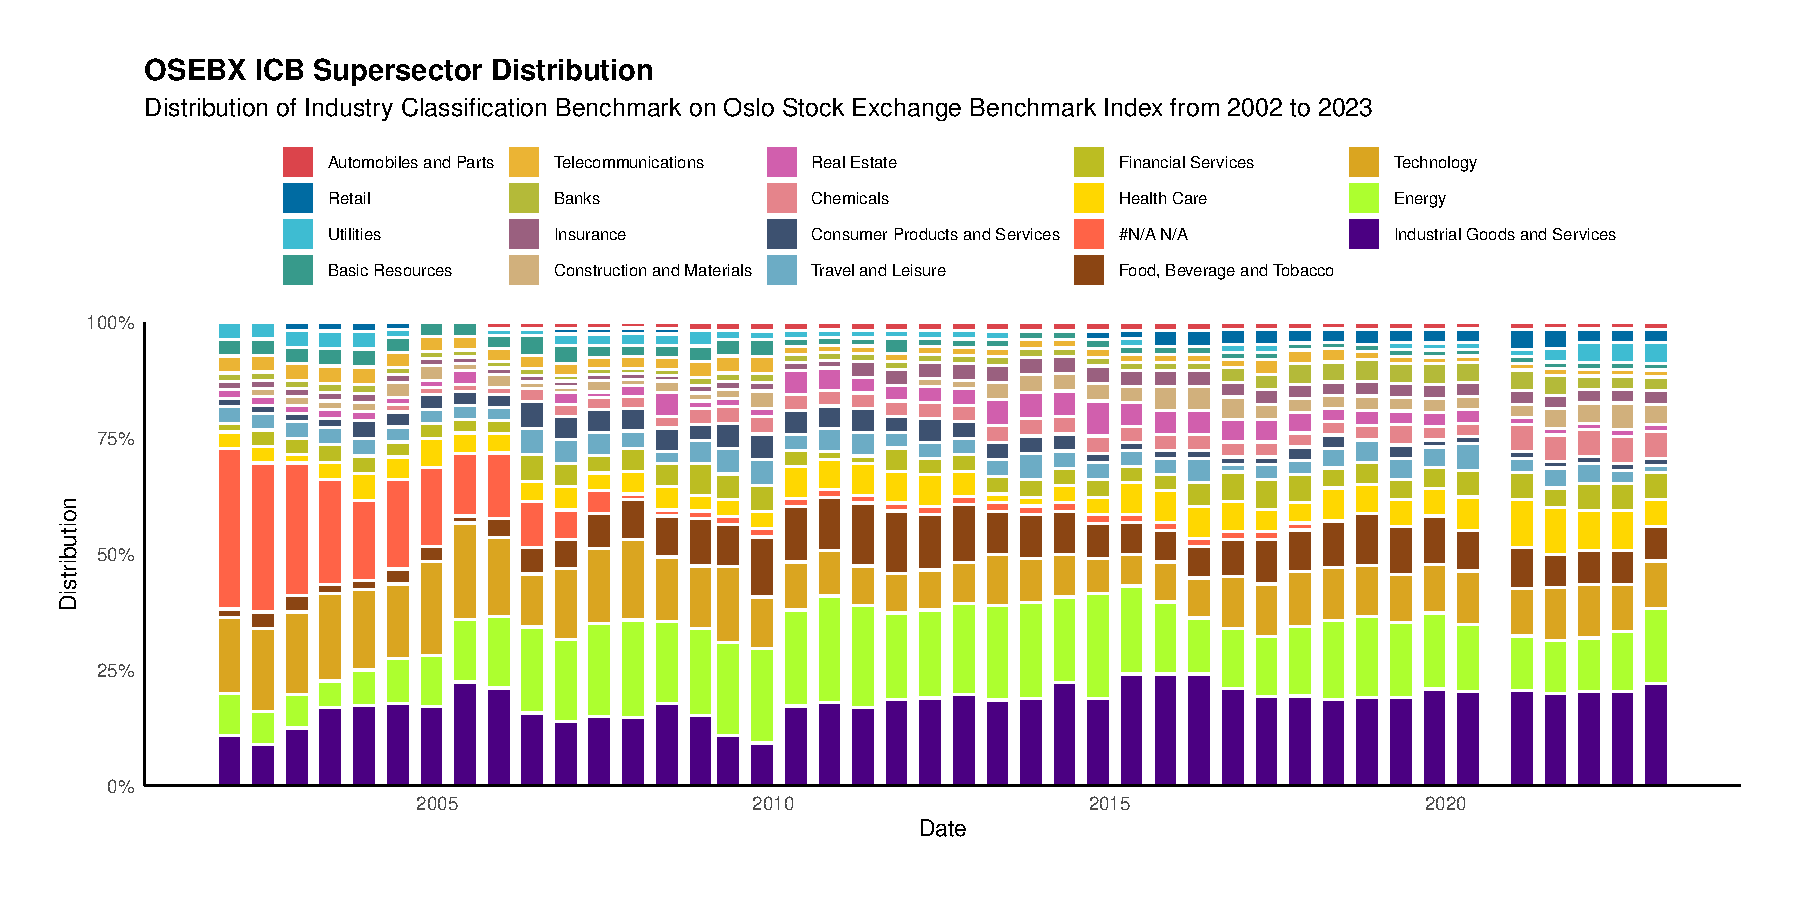
\includegraphics[width=0.9\textwidth]{images/plot_sectors.pdf}
    \caption{{OSEBX ICB Supersector Distribution over Time}}
    \subcaption*{Industry classification benchmark (ICB) for companies on OSEBX in the period from 2002 to 2023. Notice that industry and energy companies dominate OSEBX.}
    \label{Oslo Stock Exchange Benchmark Index Sector Distribution}
\end{figure}

% \begin{figure}[H]
%     \centering
%     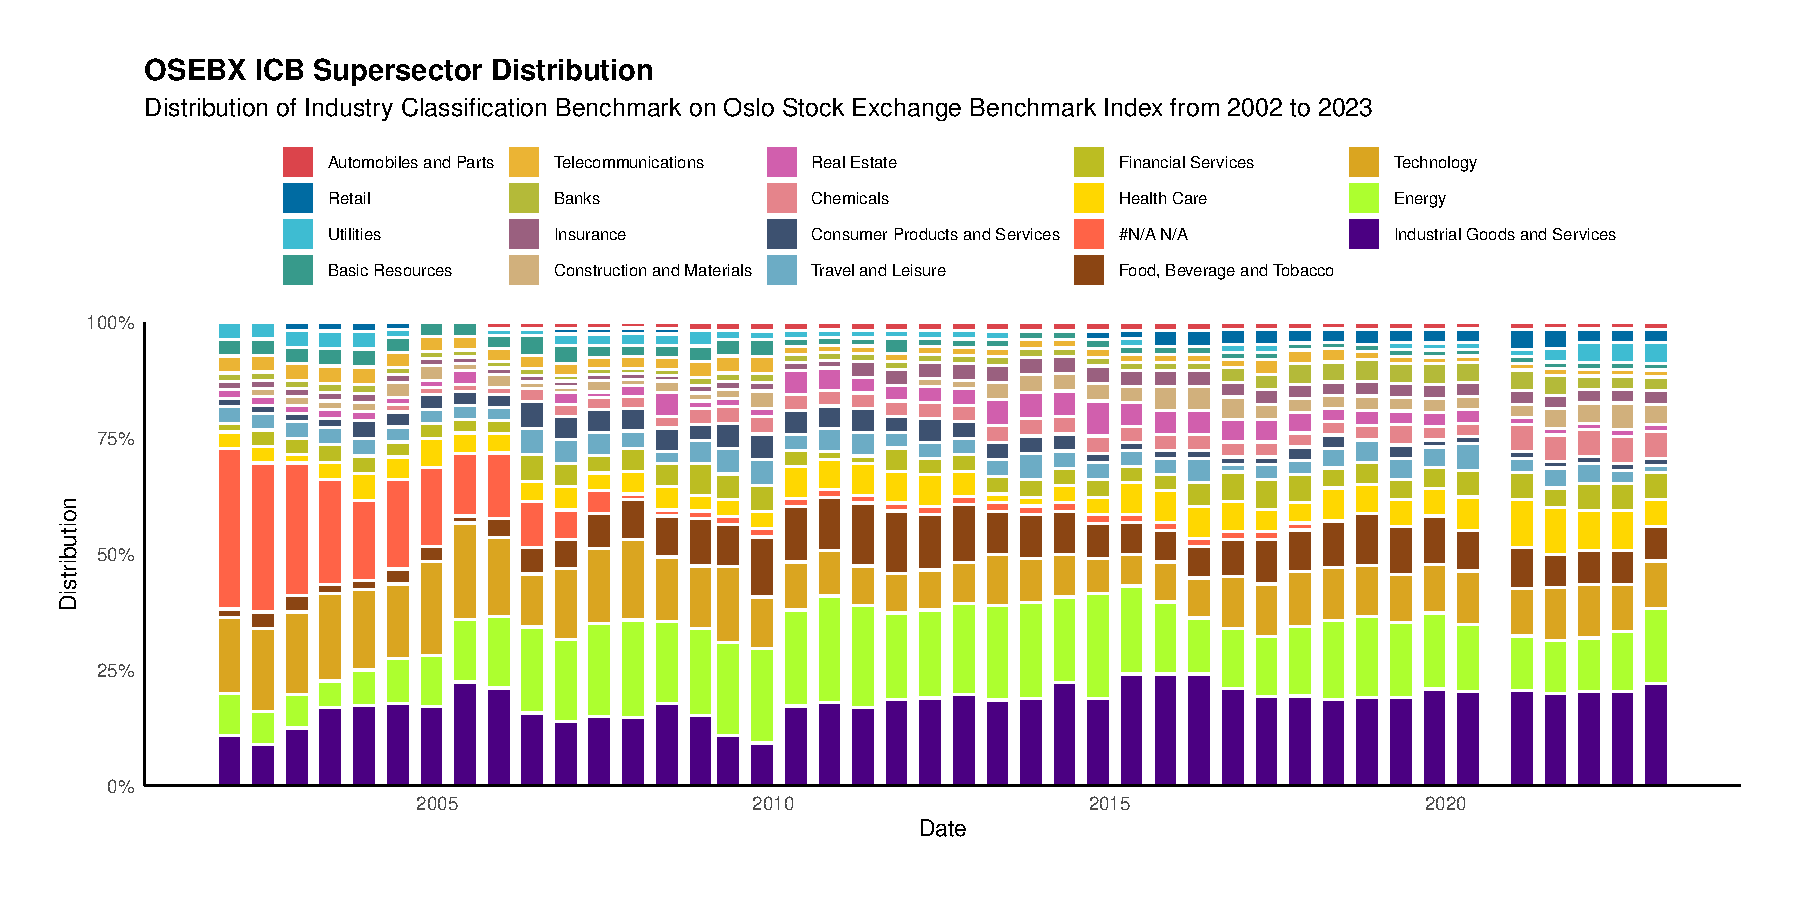
\includegraphics[width=\textwidth]{images/plot_sectors.pdf}
%     \caption{Oslo Stock Exchange Benchmark Index Sector Distribution}
%     \label{Oslo Stock Exchange Benchmark Index Sector Distribution}
% \end{figure}

% \begin{figure}[H]
%     \centering
%     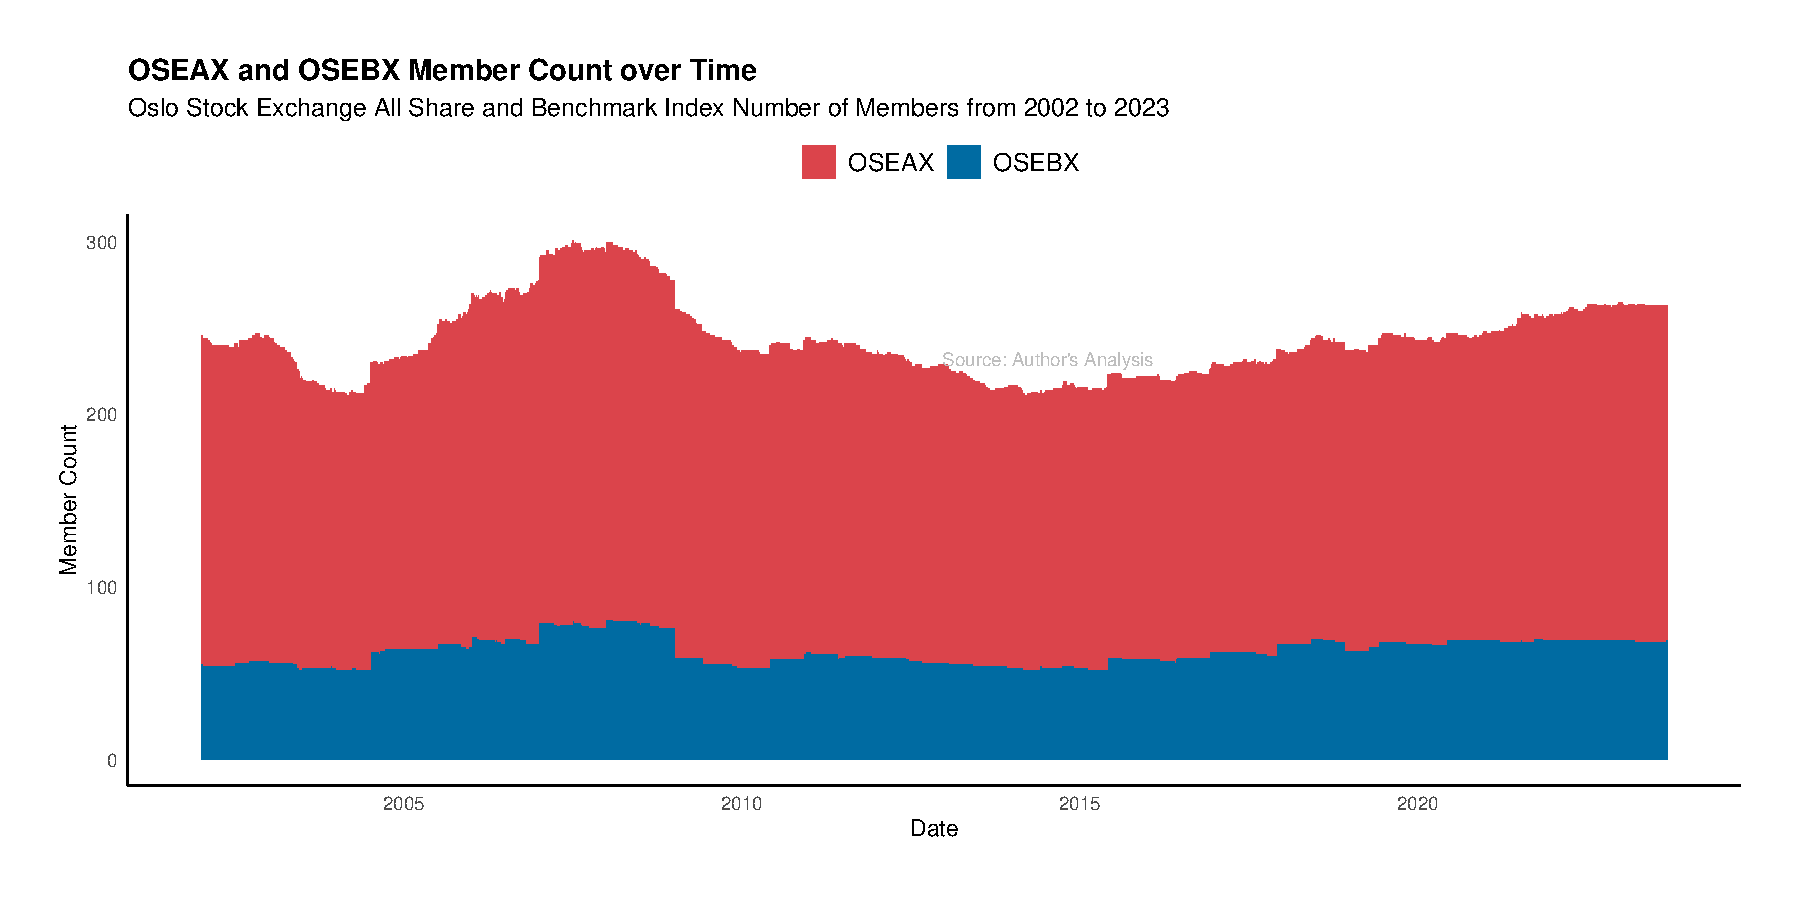
\includegraphics[width=\textwidth]{images/plot_memb_126.pdf}
%     \caption{Members over time}
%     \label{Members over time}
% \end{figure}



% Portfolios

\begin{figure}[H]
    \centering
    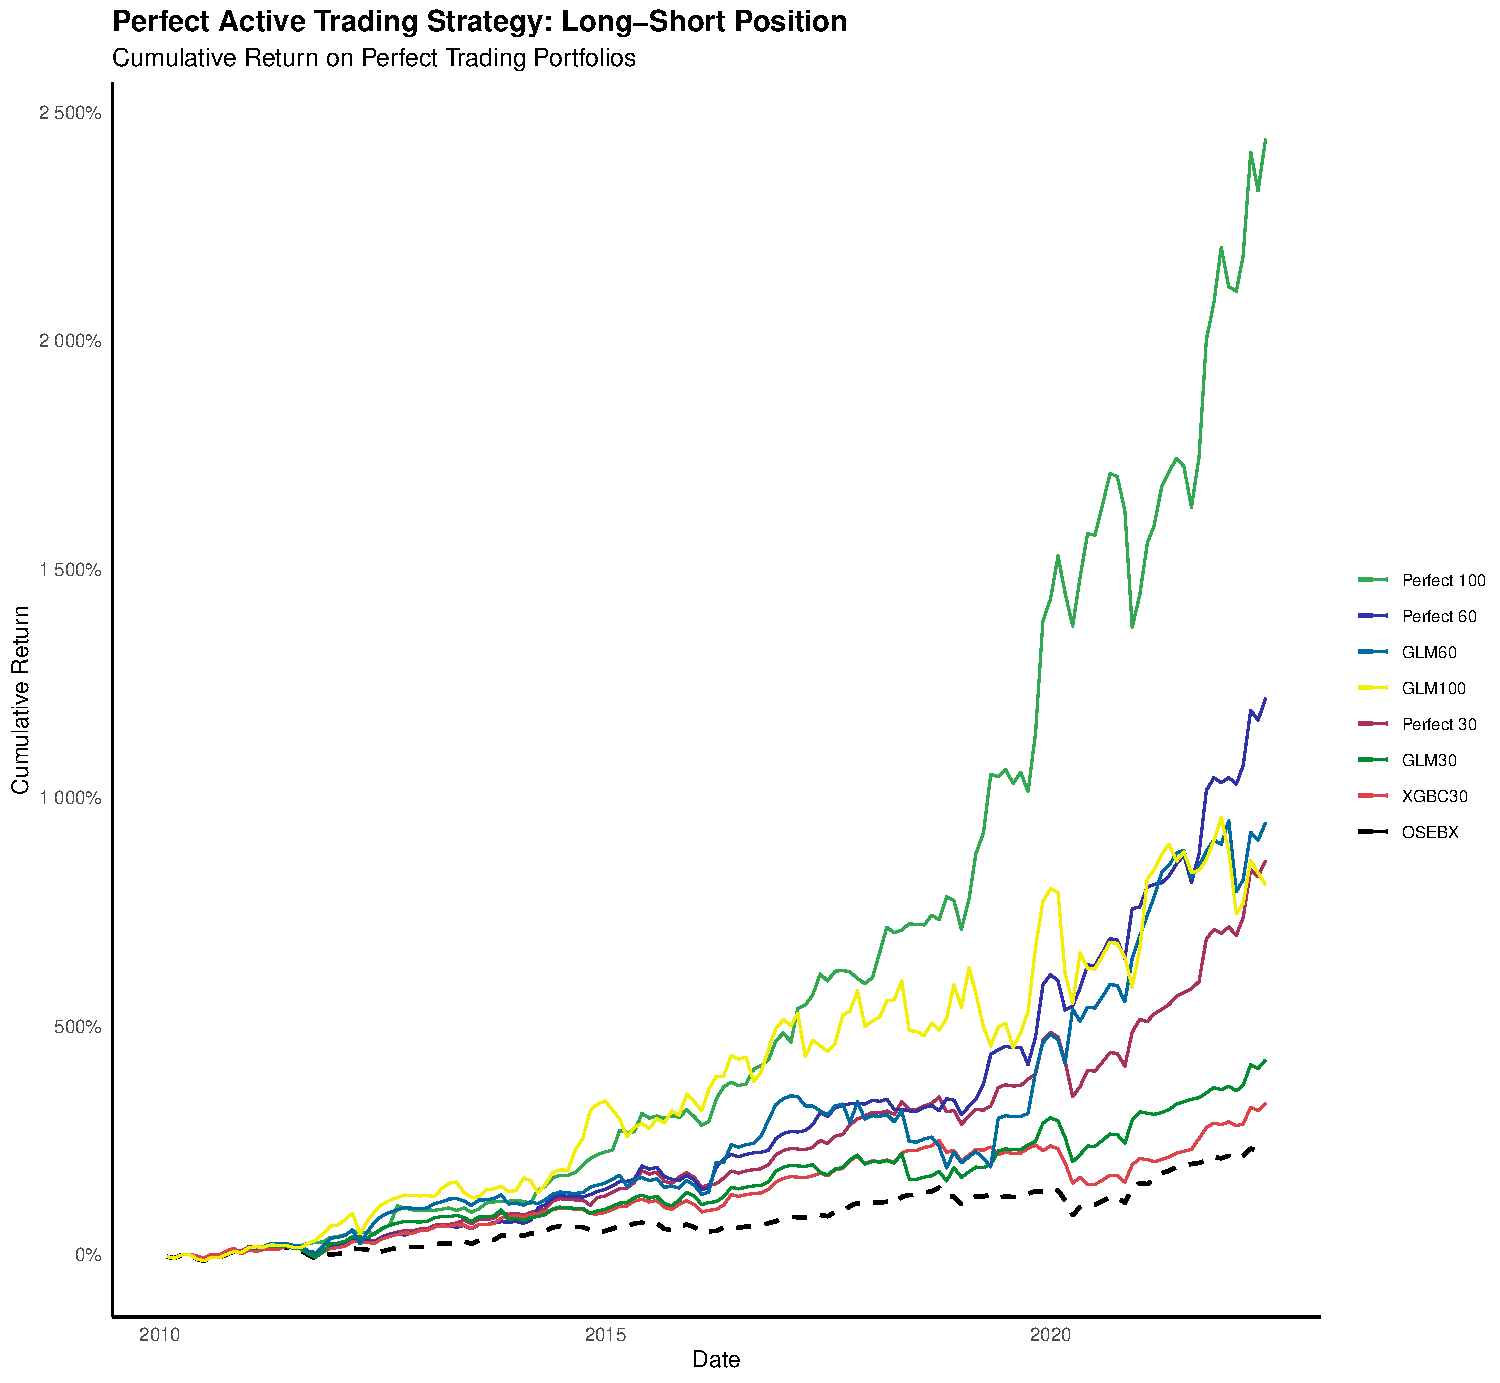
\includegraphics{images/perfect_port_monthly.pdf}
    % \vspace{1em}
    \caption{Cumulative Return Perfect Portolios}
    \subcaption*{In this figure we have included the portfolios Perfect 30, Perfect 60, and Perfect 100. Those portfolios represent the development if one had known 100\% of which companies should enter/exit OSEBX since 2010. Investing NOK 1000 on January 4th, 2010 would have grown to 25,000 on May 31st, 2022, if one knew the changes 100 days in advance of the ED, beating OSEBX by thousands of percent in cumulative return. }
    \label{fig:trading-perfect}
\end{figure}

\newpage

\begin{figure}[H]
    \centering
    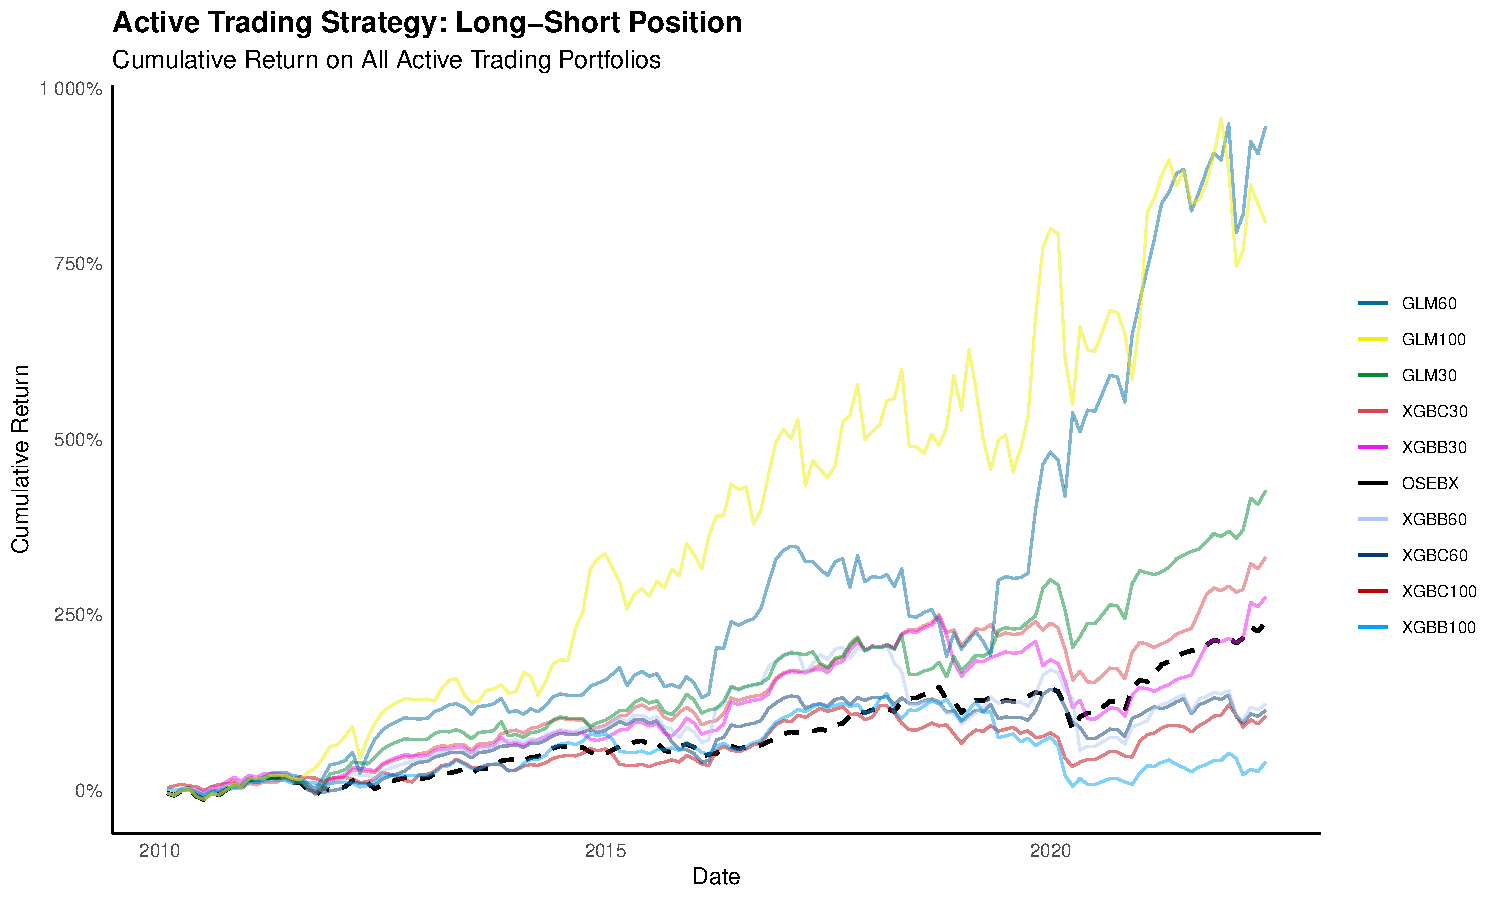
\includegraphics{images/trading_long_short_all.pdf}
    % \vspace{1em}
    \caption{Cumulative Return Long-Short Trading Strategy}
        \subcaption*{All long-short portfolios simulated are illustrated. }
    \label{fig:long-short-all}
\end{figure}

\begin{figure}[H]
    \centering
    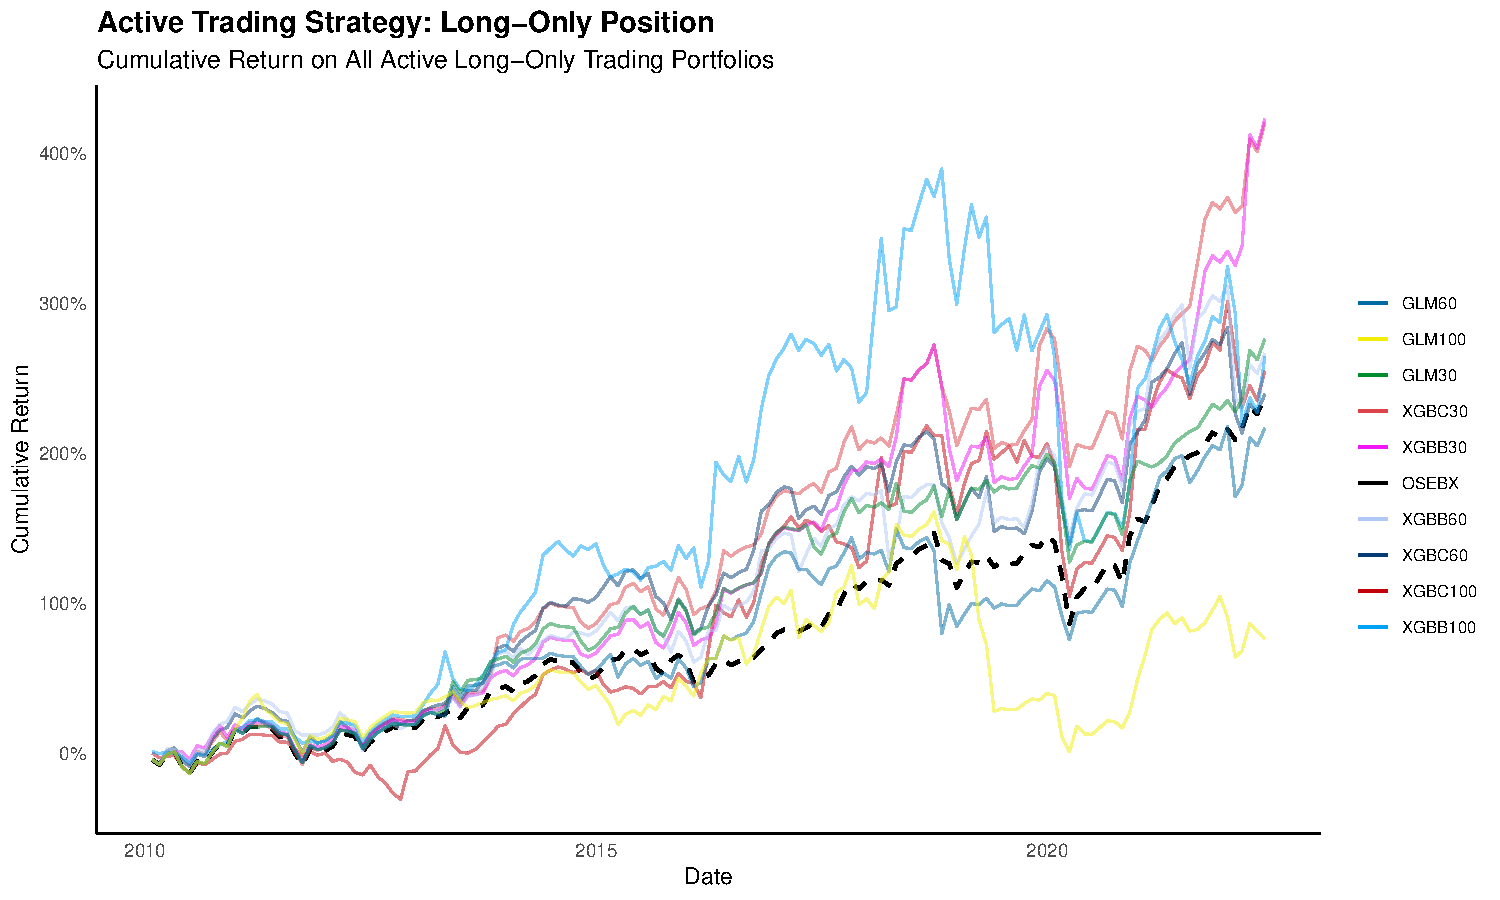
\includegraphics{images/trading_long_only_all.pdf}
    % \vspace{1em}
    \caption{Cumulative Return Long-Only Trading Strategy}
            \subcaption*{All long-only portfolios simulated are illustrated. }
    \label{fig:long-only-all}
\end{figure}

\begin{figure}[H]
    \centering
    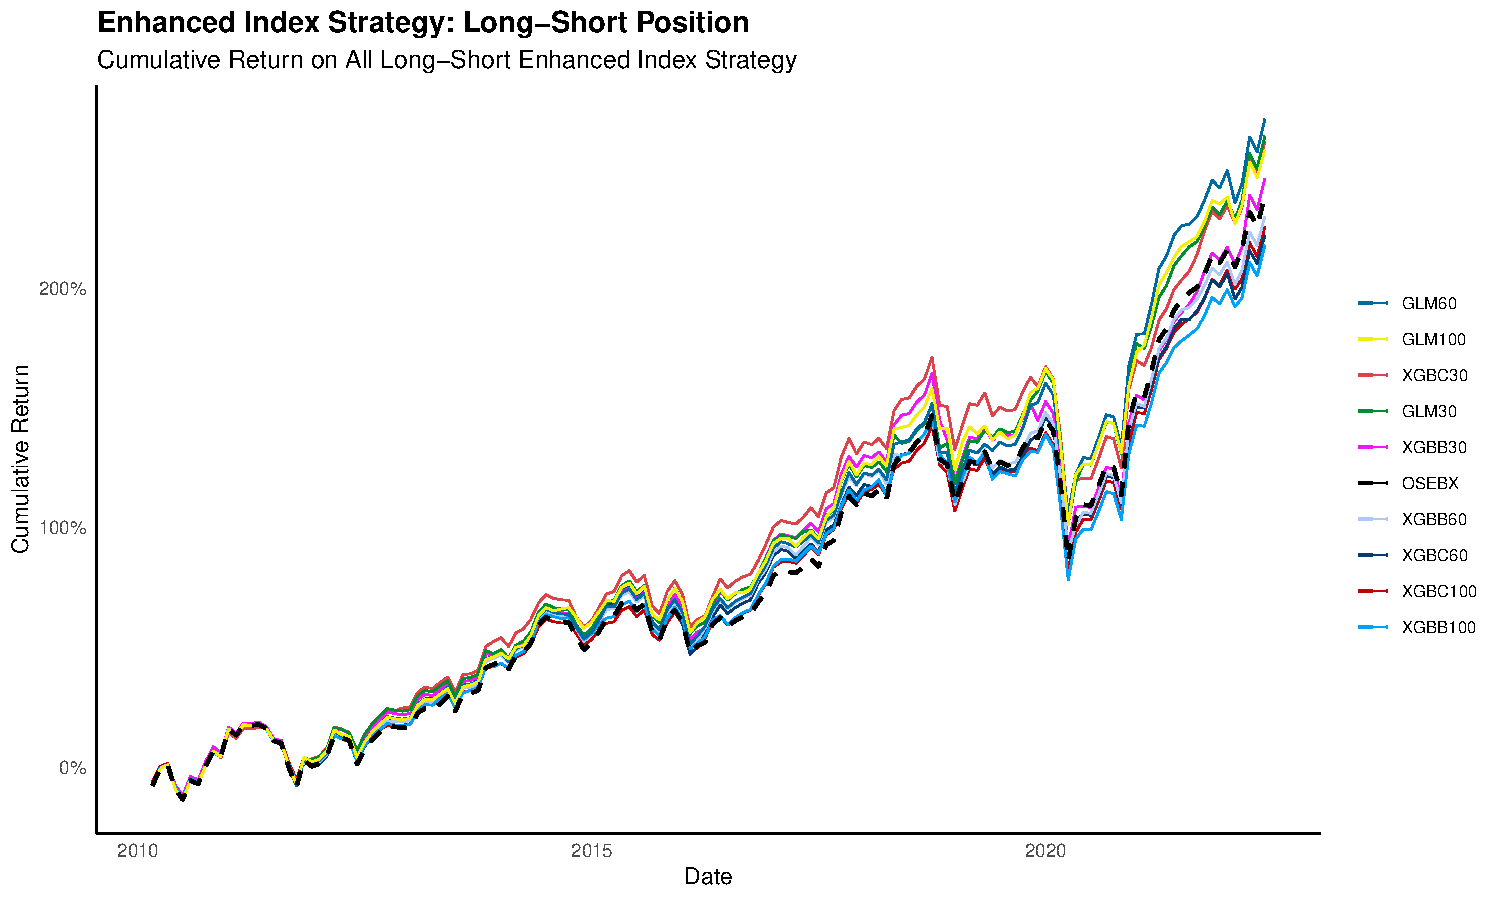
\includegraphics{images/enhanced_long_short_all.pdf}
    \caption{Cumulative Return Long-Short Enhanced Index}
            \subcaption*{All long-short enhanced portfolios simulated are illustrated. }
    \label{fig:enhanced-long-only-all}
\end{figure}

\begin{figure}[H]
    \centering
    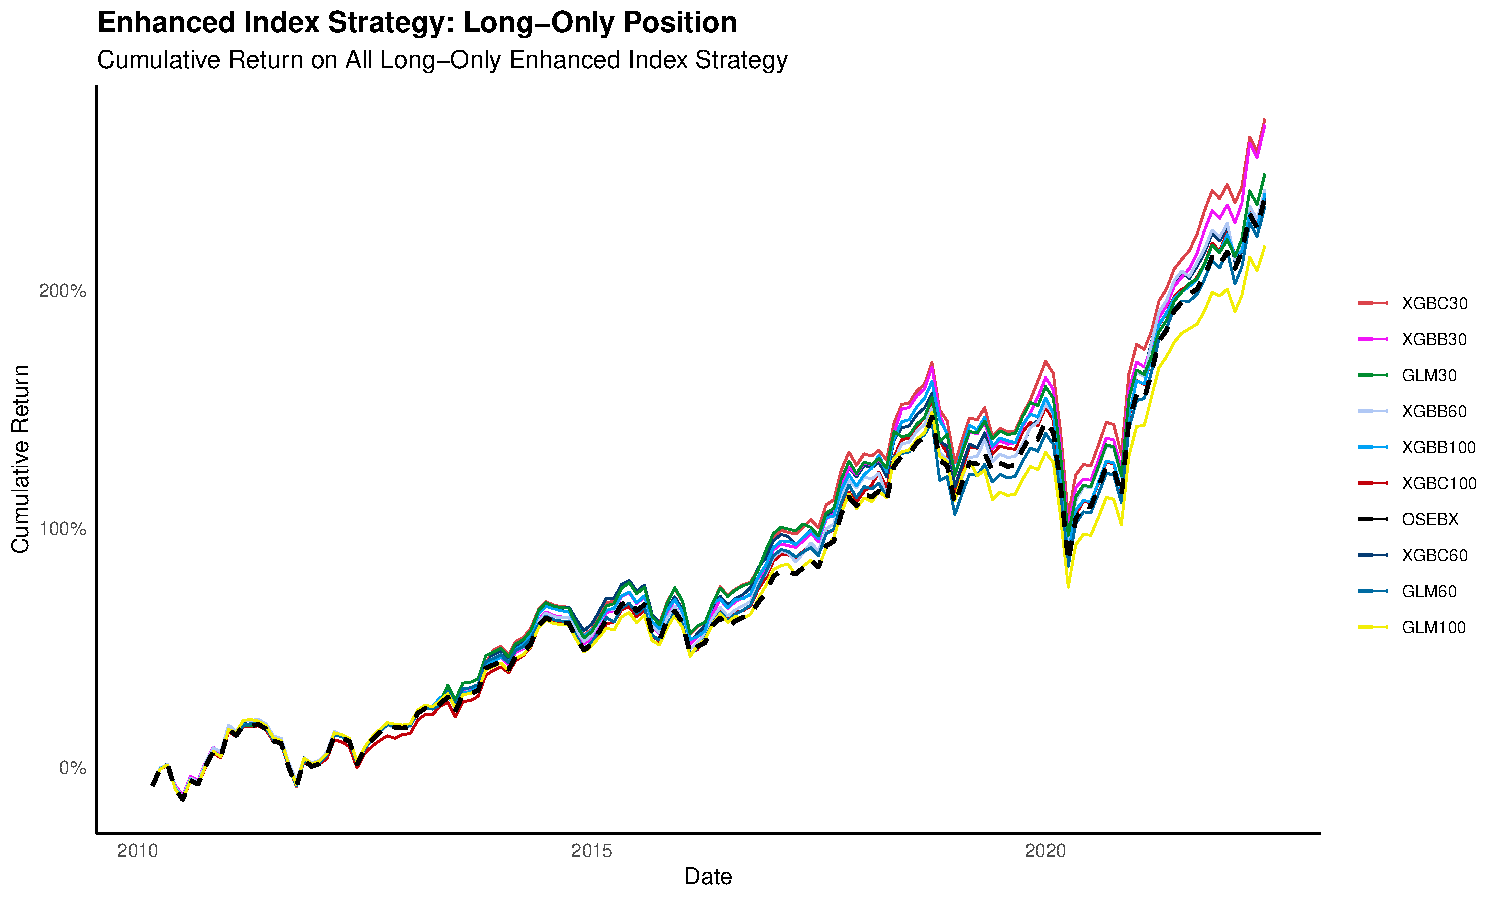
\includegraphics{images/enhanced_long_only_all.pdf}
    \caption{Cumulative Return Long-Only Enhanced Index}
                \subcaption*{All long-only enhanced portfolios simulated are illustrated. }
    \label{fig:enhanced-long-short-all}
\end{figure}
\newpage
\section{Portfolio Simulation Algorithm}
\label{APPENDIX Portfolio Simulation Algorithm}

The algorithm used when performing the portfolio simulations can be summarised as the following. All predictions come from the ML models, which are stored in a data frame including the dates of the start and end of the trading periods, and which companies are held in each trading period.

\textbf{Step 1:} Add OSEBX as a long position between each active trading period.

\textbf{Step 2:} Find VWAP for each company for each trading period start and end date, including all periods OSEBX is traded.

\textbf{Step 3:} Remove any rows with NA-values in VWAP (most present for companies in 2010 and 2011).

\textbf{Step 4:} Calculate the return on each trade, illustrated in \autoref{return_explaination_app} where $r_l$ is the return on a long position, $r_l$ is the return on short positions, $p_0$ is the VWAP at the start of the trading period and $p_1$ is the VWAP at the end of the trading period. $S_{rate}$ is the annual short rate, and $d$ is the number of days per active trading period (30, 60, or 100 days). 
\begin{equation}
\begin{aligned}
    r_l = \frac{p_1 - p_0 }{p_0} &  ,  &r_s = \frac{p_0 - p_1 }{p_0}-\frac{S_{rate}^{ann}*d}{365} 
\label{return_explaination_app}
\end{aligned}
\end{equation}

\textbf{Step 5:} Calculate the average return for each trading period, as we assume weights between the assets to be equally weighted.

\textbf{Step 6:} Define an amount of money to start with (we used 10 million). For each trading period, multiply the money at the end of the last period by the average return in that period plus 1, minus 8 bps (as we use 4 bps as transaction cost per trade, but at the end of each period we both sell the previous holdings and buy new holdings, therefore 8 bps). 

\newpage
\section{Example of Portfolio Simulation}
\label{APPENDIX Portfolio Simulation of GLM100-portfolio}
We decided to include the GLM100 portfolio as an example of a simulated portfolio. Please note that this simulation only yields portfolio size at the end of the trading periods, so in practice, we have calculated the return for each day and extracted the return from the same dates as the FF3 factors are reported (being the last date in each month). The point of this Appendix is to illustrate where the exceptional (yet risky) returns come from. 

\begin{table}[h]
\centering
\scriptsize
\begin{tabular}{llllllrrr}
  \hline
Start & End & Company & $Y_{i,t}$ & $\widehat Y_{i,t}$ & $Y_{i,t-1}$ & VWAP start & VWAP end & Return \\ 
\hline
   2010-01-04 & 2011-01-08 & OSEBX &  &  &  & 380.15 & 439.92 & 0.16 \\ 
   2011-01-11 & 2011-05-31 & AKER NO Equity & 0 & 1 & 0 & 141.72 & 153.58 & 0.08 \\ 
   2011-01-11 & 2011-05-31 & ELT NO Equity & 1 & 0 & 1 & 1.00 & 1.00 & -0.01 \\ 
   2011-01-11 & 2011-05-31 & JIN NO Equity & 0 & 0 & 1 & 19.86 & 16.40 & 0.16 \\ 
   2011-01-11 & 2011-05-31 & QFR NO Equity & 1 & 0 & 1 & 16.90 & 17.87 & -0.07 \\ 
   2011-06-01 & 2011-07-10 & OSEBX &  &  &  & 437.39 & 421.46 & -0.04 \\ 
   2011-07-13 & 2011-11-30 & MGN NO Equity & 1 & 0 & 1 & 11.21 & 5.14 & 0.53 \\ 
   2011-07-13 & 2011-11-30 & QEC NO Equity & 0 & 0 & 1 & 5.56 & 3.97 & 0.28 \\ 
   2011-12-01 & 2012-01-09 & OSEBX &  &  &  & 378.59 & 389.09 & 0.03 \\ 
   2012-01-12 & 2012-05-31 & MGN NO Equity & 0 & 0 & 1 & 6.41 & 5.21 & 0.18 \\ 
   2012-06-01 & 2013-01-08 & OSEBX & &  &  & 377.66 & 456.04 & 0.21 \\ 
   2013-01-11 & 2013-05-31 & EMGS NO Equity & 1 & 0 & 1 & 214.05 & 208.01 & 0.02 \\ 
   2013-01-11 & 2013-05-31 & SONG NO Equity & 0 & 0 & 1 & 1.00 & 1.00 & -0.01 \\ 
   2013-06-01 & 2013-07-09 & OSEBX &  &  &  & 491.71 & 482.30 & -0.02 \\ 
   2013-07-12 & 2013-11-29 & BRG NO Equity & 0 & 1 & 0 & 26.89 & 26.65 & -0.01 \\ 
   2013-07-12 & 2013-11-29 & AFG NO Equity & 1 & 0 & 1 & 61.82 & 68.07 & -0.11 \\ 
   2013-07-12 & 2013-11-29 & EMGS NO Equity & 0 & 0 & 1 & 198.11 & 157.16 & 0.20 \\ 
   2013-07-12 & 2013-11-29 & PLCS NO Equity & 1 & 0 & 1 & 432.09 & 409.77 & 0.04 \\ 
   2013-11-30 & 2014-01-07 & OSEBX &  &  &  & 542.79 & 547.04 & 0.01 \\ 
   2014-01-10 & 2014-05-30 & PLCS NO Equity & 0 & 0 & 1 & 417.46 & 341.25 & 0.17 \\ 
   2014-05-31 & 2014-07-08 & OSEBX &  &  &  & 605.26 & 619.53 & 0.02 \\ 
   2014-07-11 & 2014-11-28 & ASTK NO Equity & 0 & 0 & 1 & 18.94 & 9.14 & 0.51 \\ 
   2014-11-29 & 2015-01-06 & OSEBX &  &  &  & 566.34 & 569.98 & 0.01 \\ 
   2015-01-09 & 2015-05-29 & LSG NO Equity & 0 & 1 & 0 & 28.18 & 25.26 & -0.10 \\ 
   2015-05-30 & 2015-07-10 & OSEBX &  &  &  & 645.68 & 634.87 & -0.02 \\ 
   2015-07-13 & 2015-11-30 & LSG NO Equity & 0 & 1 & 0 & 27.35 & 31.87 & 0.17 \\ 
   2015-07-13 & 2015-11-30 & SCHB NO Equity & 1 & 1 & 0 & 184.81 & 223.98 & 0.21 \\ 
   2015-12-01 & 2016-01-09 & OSEBX &  &  &  & 632.46 & 563.75 & -0.11 \\ 
   2016-01-12 & 2016-05-31 & LSG NO Equity & 0 & 1 & 0 & 31.95 & 42.64 & 0.33 \\ 
   2016-06-01 & 2016-07-10 & OSEBX &  &  &  & 611.63 & 610.32 & -0.00 \\ 
   2016-07-13 & 2016-11-30 & AUSS NO Equity & 0 & 1 & 0 & 73.86 & 80.46 & 0.09 \\ 
   2016-07-13 & 2016-11-30 & LSG NO Equity & 1 & 1 & 0 & 41.26 & 47.08 & 0.14 \\ 
   2016-12-01 & 2017-01-08 & OSEBX &  &  &  & 662.79 & 694.57 & 0.05 \\ 
   2017-01-11 & 2017-05-31 & AUSS NO Equity & 0 & 1 & 0 & 77.41 & 71.05 & -0.08 \\ 
   2017-01-11 & 2017-05-31 & GSF NO Equity & 1 & 1 & 0 & 72.68 & 63.21 & -0.13 \\ 
   2017-06-01 & 2017-07-10 & OSEBX &  &  &  & 713.19 & 702.25 & -0.02 \\ 
   2017-07-13 & 2017-11-30 & BANO NO Equity & 1 & 1 & 0 & 81.12 & 95.05 & 0.17 \\ 
   2017-07-13 & 2017-11-30 & AUSS NO Equity & 0 & 1 & 0 & 68.92 & 70.13 & 0.02 \\ 
   2017-12-01 & 2018-01-08 & OSEBX &  &  &  & 798.41 & 834.73 & 0.05 \\ 
   2018-01-11 & 2018-05-31 & QEC NO Equity & 1 & 0 & 1 & 6.11 & 5.70 & 0.06 \\ 

 
    \midrule \multicolumn{9}{r}{{Continued on next page}} \\
   \hline
\end{tabular}
   
\end{table}



\begin{table}[H]
\centering
\scriptsize
\begin{tabular}{llllllrrr}
 \midrule \multicolumn{9}{r}{{Continuation of previous page}} \\
  \hline
Start & End & Company & $Y_{i,t}$ & $\widehat Y_{i,t}$ & $Y_{i,t-1}$ & VWAP start & VWAP end & Return \\ 
  \hline 
   2018-01-11 & 2018-05-31 & 1643322D NO Equity & 0 & 0 & 1 & 581.85 & 952.72 & -0.65 \\ 
   2018-01-11 & 2018-05-31 & B2I NO Equity & 0 & 1 & 0 & 20.69 & 18.25 & -0.12 \\ 
   2018-01-11 & 2018-05-31 & AUSS NO Equity & 1 & 1 & 0 & 65.94 & 97.46 & 0.48 \\ 
   2018-06-01 & 2018-07-10 & OSEBX &  &  &  & 880.53 & 899.13 & 0.02 \\ 
   2018-07-13 & 2018-11-30 & QEC NO Equity & 0 & 0 & 1 & 3.05 & 2.56 & 0.15 \\ 
   2018-12-01 & 2019-01-08 & OSEBX &  &  &  & 860.98 & 836.40 & -0.03 \\ 
   2019-01-11 & 2019-05-31 & RECSI NO Equity & 1 & 0 & 1 & 6.57 & 4.93 & 0.24 \\ 
   2019-01-11 & 2019-05-31 & SASNO NO Equity & 0 & 1 & 0 & 5.86 & 3.22 & -0.45 \\ 
   2019-06-01 & 2019-07-09 & OSEBX &  &  &  & 852.09 & 883.18 & 0.04 \\ 
   2019-07-12 & 2019-11-29 & RECSI NO Equity & 0 & 0 & 1 & 4.67 & 2.68 & 0.42 \\ 
   2019-11-30 & 2020-01-07 & OSEBX &  &  &  & 902.45 & 937.40 & 0.04 \\ 
   2020-01-10 & 2020-05-29 & ASA NO Equity & 0 & 1 & 0 & 122.82 & 111.89 & -0.09 \\ 
   2020-01-10 & 2020-05-29 & HAFNI NO Equity & 0 & 1 & 0 & 28.65 & 17.15 & -0.40 \\ 
   2020-01-10 & 2020-05-29 & TIETO NO Equity & 1 & 1 & 0 & 281.33 & 252.93 & -0.10 \\ 
   2020-05-30 & 2020-10-27 & OSEBX &  &  &  & 796.77 & 826.00 & 0.04 \\ 
   2020-10-30 & 2021-03-19 & BRG NO Equity & 1 & 1 & 0 & 127.72 & 184.24 & 0.44 \\ 
   2020-10-30 & 2021-03-19 & AUSS NO Equity & 0 & 1 & 0 & 64.58 & 102.50 & 0.59 \\ 
   2020-10-30 & 2021-03-19 & KAHOT NO Equity & 0 & 1 & 0 & 1.00 & 1.00 & 0.00 \\ 
   2020-10-30 & 2021-03-19 & PEXIP NO Equity & 1 & 1 & 0 & 1.00 & 1.00 & 0.00 \\ 
   2021-03-20 & 2021-04-27 & OSEBX &  &  &  & 1050.54 & 1084.14 & 0.03 \\ 
   2021-04-30 & 2021-09-17 & ASA NO Equity & 0 & 1 & 0 & 84.45 & 36.71 & -0.57 \\ 
   2021-04-30 & 2021-09-17 & AUSS NO Equity & 0 & 1 & 0 & 106.73 & 105.64 & -0.01 \\ 
   2021-04-30 & 2021-09-17 & ACC NO Equity & 0 & 1 & 0 & 16.93 & 25.20 & 0.49 \\ 
   2021-04-30 & 2021-09-17 & KAHOT NO Equity & 1 & 1 & 0 & 87.07 & 70.11 & -0.19 \\ 
   2021-04-30 & 2021-09-17 & TIETO NO Equity & 0 & 1 & 0 & 288.06 & 282.25 & -0.02 \\ 
   2021-04-30 & 2021-09-17 & SASNO NO Equity & 0 & 1 & 0 & 1.97 & 1.95 & -0.01 \\ 
   2021-09-18 & 2021-10-26 & OSEBX &  &  &  & 1141.17 & 1215.74 & 0.07 \\ 
   2021-10-29 & 2022-03-18 & AUSS NO Equity & 0 & 1 & 0 & 114.14 & 131.70 & 0.15 \\ 
   2021-10-29 & 2022-03-18 & ACC NO Equity & 1 & 1 & 0 & 31.04 & 19.44 & -0.37 \\ 
   2021-10-29 & 2022-03-18 & AUTO NO Equity & 1 & 1 & 0 & 33.69 & 34.39 & 0.02 \\ 
   2021-10-29 & 2022-03-18 & TIETO NO Equity & 0 & 1 & 0 & 260.48 & 241.40 & -0.07 \\ 
   2022-03-19 & 2022-04-26 & OSEBX &  &  &  & 1228.54 & 1226.68 & -0.00 \\ 
   2022-04-29 & 2022-09-16 & VAR NO Equity & 1 & 1 & 0 & 40.24 & 37.86 & -0.06 \\ 
   2022-04-29 & 2022-09-16 & AUSS NO Equity & 0 & 1 & 0 & 149.91 & 100.30 & -0.33 \\ 
   2022-04-29 & 2022-09-16 & GSF NO Equity & 0 & 1 & 0 & 140.78 & 108.44 & -0.23 \\ 
   2022-04-29 & 2022-09-16 & NYKD NO Equity & 1 & 1 & 0 & 37.33 & 34.20 & -0.08 \\ 
   2022-04-29 & 2022-09-16 & TIETO NO Equity & 0 & 1 & 0 & 236.26 & 265.75 & 0.12 \\ 
   2022-09-17 & 2022-10-25 & OSEBX &  &  &  & 1175.15 & 1139.47 & -0.03 \\ 
   2022-10-28 & 2023-03-17 & BORR NO Equity & 1 & 1 & 0 & 46.43 & 71.26 & 0.53 \\ 
   2022-10-28 & 2023-03-17 & PGS NO Equity & 1 & 1 & 0 & 6.68 & 9.85 & 0.47 \\ 
   2022-10-28 & 2023-03-17 & TIETO NO Equity & 0 & 1 & 0 & 245.46 & 318.92 & 0.30 \\ 
   
   \hline
\end{tabular}

     \vspace{1em}
    \caption{Explaination of the returns for portfolio GLM100}
    \subcaption*{
    In the table, we show all simulated trades from the period January 4st 2010 to March 17th, 2023. The simulated trades are based on the predictions given by the GLM100 model. The prediction is shown in column $\widehat Y_{i,t}$, whereas the column $Y_{i,t}$ shows the true classification. Here we also use the column $Y_{i,t-1}$, as we used this variable to filter out only the cases where the prediction was different from the classification in the previous period. We decided to show the development of the GLM100 portfolios because it (1) has the fewest trades and is most suited to be presented, and (2), it has exceptional returns. Following the simulation algorithm presented in \autoref{APPENDIX Portfolio Simulation Algorithm}, this table shows the simulation after Step 4.
    }
\label{glm100_prove}
\end{table}

 Please see the next page for steps 5 and step 6 from the algorithm presented in \autoref{APPENDIX Portfolio Simulation Algorithm}.

\begin{table}[H]
\centering
\scriptsize

\begin{tabular}{rllrrrr}
  \hline
 & Start & End & Period Growth Factor & Money at start & Money at end & Cumulative Return \\ 
  \hline
1 & 2010-01-04 & 2011-01-08 & 1.16 & 10000000.00 & 11564121.90 & 0.16 \\ 
  2 & 2011-01-11 & 2011-05-31 & 1.04 & 11564121.90 & 12040012.19 & 0.20 \\ 
  3 & 2011-06-01 & 2011-07-10 & 0.96 & 12040012.19 & 11591875.89 & 0.16 \\ 
  4 & 2011-07-13 & 2011-11-30 & 1.40 & 11591875.89 & 16252111.64 & 0.63 \\ 
  5 & 2011-12-01 & 2012-01-09 & 1.03 & 16252111.64 & 16689853.95 & 0.67 \\ 
  6 & 2012-01-12 & 2012-05-31 & 1.18 & 16689853.95 & 19619048.30 & 0.96 \\ 
  7 & 2012-06-01 & 2013-01-08 & 1.21 & 19619048.30 & 23675113.39 & 1.37 \\ 
  8 & 2013-01-11 & 2013-05-31 & 1.00 & 23675113.39 & 23732143.26 & 1.37 \\ 
  9 & 2013-06-01 & 2013-07-09 & 0.98 & 23732143.26 & 23258988.48 & 1.33 \\ 
  10 & 2013-07-12 & 2013-11-29 & 1.03 & 23258988.48 & 23912763.95 & 1.39 \\ 
  11 & 2013-11-30 & 2014-01-07 & 1.01 & 23912763.95 & 24080868.67 & 1.41 \\ 
  12 & 2014-01-10 & 2014-05-30 & 1.17 & 24080868.67 & 28195239.50 & 1.82 \\ 
  13 & 2014-05-31 & 2014-07-08 & 1.02 & 28195239.50 & 28837432.46 & 1.88 \\ 
  14 & 2014-07-11 & 2014-11-28 & 1.51 & 28837432.46 & 43421198.07 & 3.34 \\ 
  15 & 2014-11-29 & 2015-01-06 & 1.01 & 43421198.07 & 43665539.34 & 3.37 \\ 
  16 & 2015-01-09 & 2015-05-29 & 0.90 & 43665539.34 & 39106001.69 & 2.91 \\ 
  17 & 2015-05-30 & 2015-07-10 & 0.98 & 39106001.69 & 38420002.67 & 2.84 \\ 
  18 & 2015-07-13 & 2015-11-30 & 1.19 & 38420002.67 & 45635519.06 & 3.56 \\ 
  19 & 2015-12-01 & 2016-01-09 & 0.89 & 45635519.06 & 40641200.64 & 3.06 \\ 
  20 & 2016-01-12 & 2016-05-31 & 1.33 & 40641200.64 & 54206635.57 & 4.42 \\ 
  21 & 2016-06-01 & 2016-07-10 & 1.00 & 54206635.57 & 54047169.52 & 4.40 \\ 
  22 & 2016-07-13 & 2016-11-30 & 1.12 & 54047169.52 & 60230569.96 & 5.02 \\ 
  23 & 2016-12-01 & 2017-01-08 & 1.05 & 60230569.96 & 63070370.40 & 5.31 \\ 
  24 & 2017-01-11 & 2017-05-31 & 0.89 & 63070370.40 & 56320039.45 & 4.63 \\ 
  25 & 2017-06-01 & 2017-07-10 & 0.98 & 56320039.45 & 55411060.44 & 4.54 \\ 
  26 & 2017-07-13 & 2017-11-30 & 1.09 & 55411060.44 & 60610764.94 & 5.06 \\ 
  27 & 2017-12-01 & 2018-01-08 & 1.05 & 60610764.94 & 63319485.01 & 5.33 \\ 
  28 & 2018-01-11 & 2018-05-31 & 0.94 & 63319485.01 & 59596047.59 & 4.96 \\ 
  29 & 2018-06-01 & 2018-07-10 & 1.02 & 59596047.59 & 60807256.29 & 5.08 \\ 
  30 & 2018-07-13 & 2018-11-30 & 1.15 & 60807256.29 & 69864846.01 & 5.99 \\ 
  31 & 2018-12-01 & 2019-01-08 & 0.97 & 69864846.01 & 67814392.22 & 5.78 \\ 
  32 & 2019-01-11 & 2019-05-31 & 0.89 & 67814392.22 & 60578852.13 & 5.06 \\ 
  33 & 2019-06-01 & 2019-07-09 & 1.04 & 60578852.13 & 62740714.85 & 5.27 \\ 
  34 & 2019-07-12 & 2019-11-29 & 1.42 & 62740714.85 & 88741985.22 & 7.87 \\ 
  35 & 2019-11-30 & 2020-01-07 & 1.04 & 88741985.22 & 92107783.02 & 8.21 \\ 
  36 & 2020-01-10 & 2020-05-29 & 0.80 & 92107783.02 & 73878509.25 & 6.39 \\ 
  37 & 2020-05-30 & 2020-10-27 & 1.04 & 73878509.25 & 76529685.22 & 6.65 \\ 
  38 & 2020-10-30 & 2021-03-19 & 1.26 & 76529685.22 & 96169292.26 & 8.62 \\ 
  39 & 2021-03-20 & 2021-04-27 & 1.03 & 96169292.26 & 99168192.32 & 8.92 \\ 
  40 & 2021-04-30 & 2021-09-17 & 0.95 & 99168192.32 & 93929746.38 & 8.39 \\ 
  41 & 2021-09-18 & 2021-10-26 & 1.07 & 93929746.38 & 99992462.13 & 9.00 \\ 
  42 & 2021-10-29 & 2022-03-18 & 0.93 & 99992462.13 & 93104559.04 & 8.31 \\ 
  43 & 2022-03-19 & 2022-04-26 & 1.00 & 93104559.04 & 92889115.82 & 8.29 \\ 
  44 & 2022-04-29 & 2022-09-16 & 0.88 & 92889115.82 & 82061518.12 & 7.21 \\ 
  45 & 2022-09-17 & 2022-10-25 & 0.97 & 82061518.12 & 79504310.41 & 6.95 \\ 
  46 & 2022-10-28 & 2023-03-17 & 1.44 & 79504310.41 & 114120732.94 & 10.41 \\

   \hline
\end{tabular}
     \vspace{1em}
    \caption{Trading period returns for portfolio GLM100}
    \subcaption*{
    In this table, we complete steps 5 and 6, meaning we first have taken the average return per trade plus 1 per period "Period Growth Factor", and we have multiplied the factor by "Money at start" for each period. Here, the transaction fees are subtracted from the growth factor before multiplying with the amount of money. Please notice that the simulated portfolio uses a longer period than the period analysed in the thesis. 
    }
\label{glm100_prove}
\end{table}

\newpage
\section{FF3 Regressions against OSEBX}
\label{ff3-osebx}

\begin{table}[H] 
\centering 
\footnotesize
\begin{tabularx}{\textwidth}{XXXXXXXXXXl} 
\\[-2ex]\hline 
\hline \\[-2ex] 
 & \multicolumn{10}{c}{\textit{Dependent variable:}} \\ 
\cline{2-11} 
\\[-2ex] 
 & \multicolumn{3}{c}{GLML} & \multicolumn{3}{c}{XGBBL} & \multicolumn{3}{c}{XGBCL} & \\
 \cline{2-10}
 \\[-2ex] 
 & 30 & 60 & 100 & 30 & 60 & 100 & 30 & 60 & 100 & OSEBX \\ 
 \cline{2-10} \\
 OSEBX & 0.980$^{***}$ & 0.964$^{***}$ & 0.969$^{***}$ & 0.983$^{***}$ & 0.952$^{***}$ & 0.934$^{***}$ & 0.977$^{***}$ & 0.953$^{***}$ & 0.919$^{***}$ & 1.000$^{***}$ \\ 
  & (0.011) & (0.011) & (0.011) & (0.011) & (0.011) & (0.010) & (0.011) & (0.011) & (0.009) & (0.000) \\ 
  %& & & & & & & & & & \\ 
 SMB & $-$0.019 & $-$0.005 & $-$0.006 & $-$0.011 & $-$0.006 & 0.013 & $-$0.022$^{*}$ & $-$0.005 & 0.012 & $-$0.000 \\ 
  & (0.012) & (0.011) & (0.012) & (0.012) & (0.011) & (0.011) & (0.012) & (0.011) & (0.010) & (0.000) \\ 
  %& & & & & & & & & & \\ 
 HML & $-$0.005 & $-$0.014$^{*}$ & $-$0.015$^{*}$ & 0.010 & 0.010 & 0.007 & 0.003 & 0.008 & 0.005 & $-$0.000 \\ 
  & (0.009) & (0.008) & (0.008) & (0.009) & (0.008) & (0.008) & (0.009) & (0.008) & (0.007) & (0.000) \\ 
  %& & & & & & & & & & \\ 
 Constant & 0.001$^{*}$ & 0.001 & 0.001 & 0.001 & 0.0003 & $-$0.0001 & 0.001$^{*}$ & 0.0001 & 0.0001 & 0.000$^{***}$ \\ 
  & (0.001) & (0.0005) & (0.0005) & (0.001) & (0.0005) & (0.0005) & (0.001) & (0.0005) & (0.0004) & (0.000) \\ 
 % & & & & & & & & & & \\ 
\hline \\[-1.8ex] 
OBS & 148 & 148 & 148 & 148 & 148 & 148 & 148 & 148 & 148 & 148 \\ 
R$^{2}$ & 0.982 & 0.982 & 0.982 & 0.982 & 0.982 & 0.984 & 0.982 & 0.982 & 0.986 & 1.000 \\ 
AdjR$^{2}$ & 0.981 & 0.982 & 0.982 & 0.981 & 0.982 & 0.983 & 0.982 & 0.982 & 0.985 & 1.000 \\ 

\hline 
\hline \\[-2ex] 
\textit{Note:}  & \multicolumn{10}{r}{$^{*}$p$<$0.1; $^{**}$p$<$0.05; $^{***}$p$<$0.01} \\ 
\end{tabularx}
\vspace{1em}
\caption{{FF3 Regression: Long-Short Enhanced Portfolios against OSEBX}} 
\subcaption*{The table shows the regression summary against OSEBX. This is the enhanced long-short portfolios.
}
\label{FF3-long-short-enhanced-osebx} 
\end{table} 



\begin{table}[H] 
\centering 
\footnotesize
\begin{tabularx}{\textwidth}{XXXXXXXXXXl} 
\\[-2ex]\hline 
\hline \\[-2ex] 
 & \multicolumn{10}{c}{\textit{Dependent variable:}} \\ 
\cline{2-11} 
\\[-2ex] 
 & \multicolumn{3}{c}{GLM} & \multicolumn{3}{c}{XGBB} & \multicolumn{3}{c}{XGBC} & \\
 \cline{2-10}
 \\[-2ex] 
 & 30 & 60 & 100 & 30 & 60 & 100 & 30 & 60 & 100 & OSEBX \\ 
 \cline{2-10} \\
 OSEBX & 0.995$^{***}$ & 1.005$^{***}$ & 0.997$^{***}$ & 0.993$^{***}$ & 0.983$^{***}$ & 0.981$^{***}$ & 0.991$^{***}$ & 0.990$^{***}$ & 0.969$^{***}$ & 1.000$^{***}$ \\ 
  & (0.011) & (0.011) & (0.011) & (0.011) & (0.011) & (0.011) & (0.011) & (0.011) & (0.011) & (0.000) \\ 
  %& & & & & & & & & & \\ 
 SMB & $-$0.010 & 0.013 & 0.017 & 0.011 & 0.014 & 0.025$^{**}$ & 0.008 & 0.013 & 0.023$^{*}$ & $-$0.000 \\ 
  & (0.012) & (0.012) & (0.012) & (0.012) & (0.012) & (0.012) & (0.012) & (0.012) & (0.012) & (0.000) \\ 
  %& & & & & & & & & & \\ 
 HML & 0.005 & $-$0.006 & $-$0.005 & 0.014 & 0.003 & 0.005 & 0.006 & 0.0003 & 0.003 & $-$0.000 \\ 
  & (0.009) & (0.009) & (0.009) & (0.009) & (0.009) & (0.009) & (0.009) & (0.009) & (0.009) & (0.000) \\ 
  %& & & & & & & & & & \\ 
 Constant & 0.0004 & $-$0.0003 & $-$0.001 & 0.001 & 0.00003 & $-$0.0002 & 0.001 & $-$0.0001 & $-$0.0001 & 0.000$^{***}$ \\ 
  & (0.001) & (0.001) & (0.001) & (0.001) & (0.001) & (0.001) & (0.001) & (0.001) & (0.001) & (0.000) \\ 
 % & & & & & & & & & & \\ 
\hline \\[-1.8ex] 
OBS & 148 & 148 & 148 & 148 & 148 & 148 & 148 & 148 & 148 & 148 \\ 
R$^{2}$ & 0.982 & 0.982 & 0.982 & 0.982 & 0.982 & 0.982 & 0.982 & 0.982 & 0.982 & 1.000 \\ 
AdjR$^{2}$ & 0.981 & 0.982 & 0.982 & 0.981 & 0.981 & 0.981 & 0.981 & 0.981 & 0.981 & 1.000 \\ 

\hline 
\hline \\[-2ex] 
\textit{Note:}  & \multicolumn{10}{r}{$^{*}$p$<$0.1; $^{**}$p$<$0.05; $^{***}$p$<$0.01} \\ 
\end{tabularx}
\vspace{1em}
\caption{{FF3 Regression: Long-Only Enhanced Portfolios against OSEBX}} 
\subcaption*{The table shows the regression summary against OSEBX. This is the enhanced long-only portfolios.
}
\label{FF3-long-only-enhanced-osebx} 
\end{table} 


\begin{table}[H] 
\centering 
\footnotesize
\begin{tabularx}{\textwidth}{XXXXXXXXXXl} 
\\[-2ex]\hline 
\hline \\[-2ex] 
 & \multicolumn{10}{c}{\textit{Dependent variable:}} \\ 
\cline{2-11} 
\\[-2ex] 
 & \multicolumn{3}{c}{GLML} & \multicolumn{3}{c}{XGBBL} & \multicolumn{3}{c}{XGBCL} & \\
 \cline{2-10}
 \\[-2ex] 
 & 30 & 60 & 100 & 30 & 60 & 100 & 30 & 60 & 100 & OSEBX \\ 
 \cline{2-10} \\

 OSEBX & 0.872$^{***}$ & 0.562$^{***}$ & 0.469$^{***}$ & 0.900$^{***}$ & 0.495$^{***}$ & 0.419$^{***}$ & 0.901$^{***}$ & 0.690$^{***}$ & 0.307$^{***}$ & 1.000$^{***}$ \\ 
  & (0.071) & (0.143) & (0.146) & (0.060) & (0.113) & (0.101) & (0.044) & (0.076) & (0.084) & (0.000) \\ 
  %& & & & & & & & & & \\ 
 SMB & $-$0.130$^{*}$ & $-$0.115 & $-$0.109 & $-$0.063 & $-$0.044 & 0.160 & $-$0.085$^{*}$ & $-$0.027 & 0.122 & $-$0.000 \\ 
  & (0.074) & (0.149) & (0.152) & (0.063) & (0.118) & (0.105) & (0.046) & (0.079) & (0.088) & (0.000) \\ 
 % & & & & & & & & & & \\ 
 HML & $-$0.042 & $-$0.213$^{*}$ & $-$0.142 & 0.048 & 0.083 & 0.005 & 0.009 & 0.037 & 0.014 & $-$0.000 \\ 
  & (0.054) & (0.109) & (0.112) & (0.046) & (0.087) & (0.077) & (0.034) & (0.058) & (0.064) & (0.000) \\ 
  %& & & & & & & & & & \\ 
 Constant & 0.006$^{*}$ & 0.013$^{**}$ & 0.014$^{**}$ & 0.003 & 0.004 & $-$0.003 & 0.004$^{*}$ & 0.0005 & 0.0001 & 0.000$^{***}$ \\ 
  & (0.003) & (0.006) & (0.007) & (0.003) & (0.005) & (0.005) & (0.002) & (0.003) & (0.004) & (0.000) \\ 
  %& & & & & & & & & & \\ 
\hline \\[-1.8ex] 
Obs. & 147 & 147 & 147 & 147 & 147 & 147 & 147 & 147 & 147 & 147 \\ 
R$^{2}$ & 0.515 & 0.109 & 0.072 & 0.621 & 0.131 & 0.127 & 0.748 & 0.378 & 0.103 & 1.000 \\ 
AdjR$^{2}$ & 0.505 & 0.090 & 0.052 & 0.613 & 0.113 & 0.109 & 0.742 & 0.365 & 0.084 & 1.000 \\ 


\hline 
\hline \\[-2ex] 
\textit{Note:}  & \multicolumn{10}{r}{$^{*}$p$<$0.1; $^{**}$p$<$0.05; $^{***}$p$<$0.01} \\ 
\end{tabularx}
\vspace{1em}
\caption{{FF3 Regression: Long-Short Active Portfolios against OSEBX}} 
\subcaption*{The table shows the regression summary against OSEBX. This is the active long-short portfolios.
}
\label{FF3-long-short-active-osebx} 
\end{table} 



\begin{table}[H] 
\centering 
\footnotesize
\begin{tabularx}{\textwidth}{XXXXXXXXXXl} 
\\[-2ex]\hline 
\hline \\[-2ex] 
 & \multicolumn{10}{c}{\textit{Dependent variable:}} \\ 
\cline{2-11} 
\\[-2ex] 
 & \multicolumn{3}{c}{GLM} & \multicolumn{3}{c}{XGBB} & \multicolumn{3}{c}{XGBC} & \\
 \cline{2-10}
 \\[-2ex] 
 & 30 & 60 & 100 & 30 & 60 & 100 & 30 & 60 & 100 & OSEBX \\ 
 \cline{2-10} \\

 OSEBX & 0.984$^{***}$ & 1.029$^{***}$ & 0.991$^{***}$ & 0.958$^{***}$ & 0.882$^{***}$ & 0.741$^{***}$ & 0.953$^{***}$ & 0.946$^{***}$ & 0.652$^{***}$ & 1.000$^{***}$ \\ 
  & (0.039) & (0.068) & (0.103) & (0.057) & (0.078) & (0.118) & (0.052) & (0.061) & (0.116) & (0.000) \\ 
  %& & & & & & & & & & \\ 
 SMB & $-$0.032 & 0.068 & 0.192$^{*}$ & 0.049 & 0.096 & 0.302$^{**}$ & 0.037 & 0.074 & 0.204$^{*}$ & $-$0.000 \\ 
  & (0.040) & (0.071) & (0.107) & (0.059) & (0.081) & (0.123) & (0.054) & (0.064) & (0.121) & (0.000) \\ 
  %& & & & & & & & & & \\ 
 HML & 0.016 & $-$0.041 & $-$0.076 & 0.059 & 0.023 & 0.033 & 0.021 & $-$0.003 & 0.041 & $-$0.000 \\ 
  & (0.030) & (0.052) & (0.079) & (0.043) & (0.060) & (0.090) & (0.040) & (0.047) & (0.089) & (0.000) \\ 
  %& & & & & & & & & & \\ 
 Constant & 0.002 & $-$0.001 & $-$0.006 & 0.004 & 0.001 & $-$0.0004 & 0.003 & $-$0.0002 & 0.002 & 0.000$^{***}$ \\ 
  & (0.002) & (0.003) & (0.005) & (0.003) & (0.004) & (0.005) & (0.002) & (0.003) & (0.005) & (0.000) \\ 
  %& & & & & & & & & & \\ 
\hline \\[-1.8ex] 
Obs. & 147 & 147 & 147 & 147 & 147 & 147 & 147 & 147 & 147 & 147 \\ 
R$^{2}$ & 0.822 & 0.620 & 0.409 & 0.678 & 0.487 & 0.255 & 0.709 & 0.635 & 0.207 & 1.000 \\ 
AdjR$^{2}$ & 0.818 & 0.612 & 0.397 & 0.672 & 0.476 & 0.239 & 0.703 & 0.627 & 0.190 & 1.000 \\ 


\hline 
\hline \\[-2ex] 
\textit{Note:}  & \multicolumn{10}{r}{$^{*}$p$<$0.1; $^{**}$p$<$0.05; $^{***}$p$<$0.01} \\ 
\end{tabularx}
\vspace{1em}
\caption{{FF3 Regression: Long-Only Active Portfolios against OSEBX}} 
\subcaption*{The table shows the regression summary against OSEBX. This is the active long-only portfolios.
}
\label{FF3-long-only-active-osebx} 
\end{table} 






\end{appendices}



% End document 
\end{document}
